\lchapter[visu]{Graph visualization application}

\section{Introduction}

\p{Data collection, analysis and visualization}
Being able to process an extensive collection of different datasets representing complex systems and store them in a common format opens the doors to different ways to analyze and visualize these systems. The first part, the data collection and storage process, was handled in the previous chapter with a special focus on open-source projects. This chapter, instead, is dedicated to the explanation of how we approached part of the second problem: the data visualization.

\p{Browser-based application}
As already introduced in \vref{sec:case/arch}, being able to take a dataset and produce a meaningful visualization is only a part of the problem. Many other factors incur when developing an application to solve this particular issue, as for example, ease of use, compatibility, performance, distribution, etc. For these and other reasons reported in the referenced chapter, we choose to build a new visualization application from scratch running completely in a web browser.

\p{Limitations}
Beside the obvious advantages for the end user concerning the installation and update process, this decision also presents some interesting challenges. The main class of problems we will encounter are probably due to the limitations imposed by the platform (in this case, the browser). These are mainly related to the sandboxed execution environment but can span other domains as well, such as the development environment (JavaScript is the only language supported out of the box), or performance concerns (again, JavaScript is an interpreted scripting language).

\p{Structure of this chapter}
In this chapter we first present the analysis of the visualization application to implement (\ref{sec:visu/analysis}), afterwards we proceed to the discussion of the design phase (\ref{sec:visu/design}), and provide interesting insights into the actual implementation (\ref{sec:visu/implementation}). Finally, in the last section (\ref{sec:visu/results}), we present the results of our work by analyzing the developed layout strategies and by evaluating the performances of the application.

\section{Analysis}
\label{sec:visu/analysis}

\subsection{Multi-domain visualization}

\p{Lack of support}
While different graph visualization applications already exist, most of them supporting a notable set of features, they all lack explicit support for multi-domain data. With this being one of the main reasons to develop a new application from scratch, we obviously concentrated our developments efforts in this area.

\p{Exploiting existing art}
In \cite{graphvisu} we analyzed the current state of the art regarding general graph visualization techniques, and we explored different ways to apply existing algorithms to layered multi-domain graphs. The visualization application shall offer a generic way to hook up existing layout algorithms with multi-domain graphs by using different approaches.

\p{Layout algorithms}
We approached this problem by modeling a layout algorithm as presented in \vref{fig:layout}; a layout algorithm is a function taking a list of nodes and a list of edges as arguments, and returns a list of positions at which the nodes shall be placed. A layout algorithm should not be concerned with the multi-domain nature of the graph.\footnote{Although, as we will see, this is not always the case: specialized algorithms can make use of additional metadata to better optimize the layout.}

\p{Layout strategies}
A layout \emph{strategy} instead, is a function which takes a list of nodes, a list of edges, and a list of domains to which the different nodes belong. Its result is, as for the layout algorithm, a list of positions at which the nodes shall be placed. A strategy works by preprocessing the input data so that it can be passed to one or more layout algorithms. Once the layout algorithms did their work, the strategy postprocesses the results and returns a coherent list of positions for each node in the graph. A possible layout strategy internal is presented in \vref{fig:strategy}.

\begin{figure}
  \begin{adjustwidth}{-0.25mm}{-0.6mm}
  \subfloat[Layout algorithm]{%
		\label{fig:layout}%
		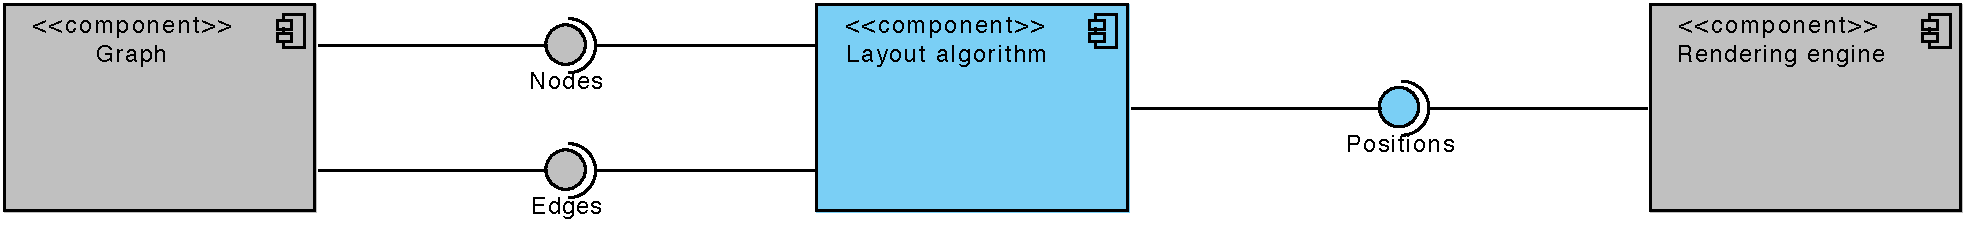
\includegraphics[width=\linewidth]{images/diagrams/comp-layout}
  }\end{adjustwidth}

  \begin{adjustwidth}{-5mm}{-4.7mm}
	\subfloat[Layout strategy]{%
		\label{fig:strategy}%
		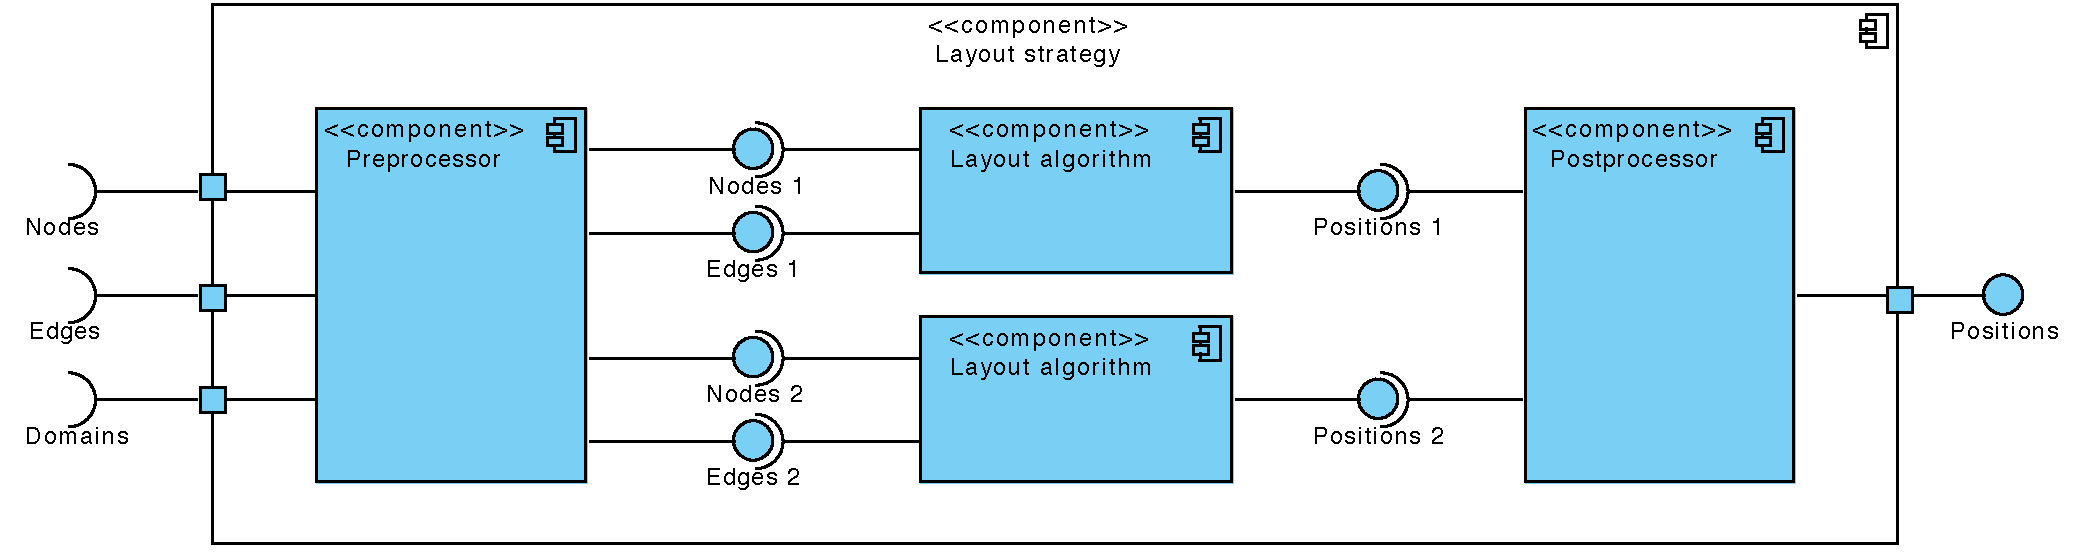
\includegraphics[width=\linewidth]{images/diagrams/comp-strategy}
	}
  \end{adjustwidth}
  \caption[The components of the Strategy/Layout model.]{A layout algorithm and a possible internal representation of a layout strategy making use of two generic layout algorithms. For the sake of simplicity, the two external components in the first subfigure, namely the \emph{Graph} and the \emph{Rendering engine}, were omitted from the second subfigure.}
  \label{fig:layout-strategy}
\end{figure}

\p{Advantages of the model}
This model to draw multi-domain graphs has the big advantage to allow the reuse of the extended academic background in graph layout algorithms, while allowing new approaches of their application to multi-domain graphs to be developed. The flexibility is not constrained as a layout strategy could possibly just be a totally new, multi-domain aware, layout algorithm and not follow the internal description presented in the previous paragraph.

\subsection{Use case diagram}

\p{Introduction}
\Vref*{fig:uc-visu} shows the use case diagram for the data visualization web application. The diagram only contains the main use cases and is far from complete. For the purposes of our analysis it is sufficient as it allows us to describe the main user interaction modalities and helps explain the architectural design in the next chapter.

\begin{figure}
  \centering
  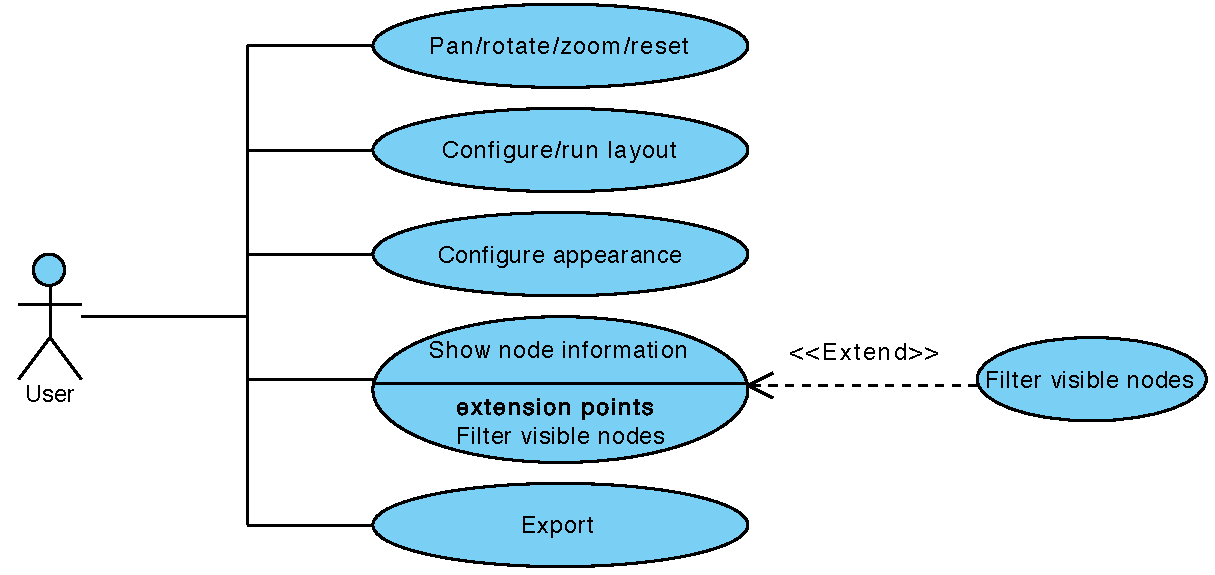
\includegraphics[width=.8\linewidth]{images/diagrams/uc-visu}
  \caption[Use case diagram for the data visualization web application.]{Use case diagram for the data visualization web application.}
  \label{fig:uc-visu}
\end{figure}

\p{Initial conditions}
For all the presented use cases, we suppose that the users starts at the initial screen of the visualization application, with a graph renderer on the screen. As this screen can be reached from different links in the data acquisition application, this first step can be considered a \emph{Visualize graph} \gls{uc} to be added to the use case diagram in \vref{fig:uc-acquisition}.

\p{Actors and use cases}
The only actor interacting with the application is the end user and its role is self explanatory. The different represented use cases can be described as follows:

\begin{description}
  \item[Pan/rotate/zoom/reset] This use case (or group of use cases) allows to interact with the graph position, very much like with an interactive online map. The available actions allow to \emph{pan} the graph (2-dimensional displacement along the $x$ and $y$ axis), \emph{rotate} the graph (3-dimensional rotation around the graph center), \emph{zoom} in and out, and \emph{reset} the view to the initial conditions.
  \item[Configure/run layout] This could have been, again, split into two or more use cases, but we consider the whole process of selecting a strategy, selecting a layout, modifying the configuration, and running the setup as a single use case.
  \item[Configure appearance] This use case allows the user to configure the graph visualization properties (node sizes, node colors, edge direction indicators, background color, transparency, \ldots) to suit its needs.
  \item[Show node information] As each node can contain one or more attributes, this use case allows to select a node for which the attributes shall be displayed. In addition to attributes, some basic metrics are displayed as well.
  \item[Filter visible nodes] Once a node is selected and its attributes displayed as per the precedent use case, the user can optionally filter the graph in order to display only the \nth{1}, \nth{2} or \nth{3} degree neighbors.
  \item[Export] This use case allows to export the current view. Different exporting options should be available for the user to choose.
\end{description}

\subsection{Extensibility}

\p{Pluggable architecture}
A point which naturally derives from the layout/strategies model previously presented is the need for an extensible architecture so that new layouts and strategies can be plugged in easily.

\p{Extension points}
In the application, we can identify three interfaces which have to be aware of this:
\begin{enumerate}
  \item \textbf{Layout algorithms} have to implement a specific interface and shall be supported by the system in an interchangeable way.
  \item The same applies to \textbf{strategies}, which shall be interchangeable as well.
  \item The third interface sits between strategies and layout algorithms. A strategy using one or more layouts algorithms in its internals shall support any layout algorithm implementation. There are some combinations of strategies and layout algorithms which may not make sense because of the form of the resulting drawing. This point shall rather be addressed in the user interface, rather than imposing limits on the architecture itself.
\end{enumerate}

\p{Configurability}
As each strategy or layout algorithm may require a different set of configuration options, the application shall as well provide means to specify these settings and expose them in a meaningful way to the end user.

\p{Other extension points}
The single most important extension point is clearly the layout engine, but the application presents many other possible plugin points for users to modify the default behavior or hook up their custom implementations. The following is a non-exhaustive list of other extension points which should be considered during the design and the implementation of the application:

\begin{itemize}
  \item The graph reading \gls{api} could support multiple input formats by using plugins (and auto-negotiation) to create a model from a source descriptor.
  \item Similarly, a pluggable exporting \gls{api} would allow the user to export to different formats by integrating the appropriate plugin.
  \item The node filtering can also be delegated to specific plugins.
  \item Different metrics can be calculated by different plugins as well and be displayed with the other node attributes (for node metrics) or in a dedicated widget.
  \item As discovered later in the development process, but reported here for convenience, a pluggable graph visualization engine could also help in supporting multiple, differently-performing, graph renderings (e.g., a ``preview'' renderer and a ``high-definition'' renderer).
\end{itemize}

\section{Design}
\label{sec:visu/design}

\afterpage{%
  \begin{a3page}
  \begin{figure}[h]
    \centering
    \vspace{-2cm}
    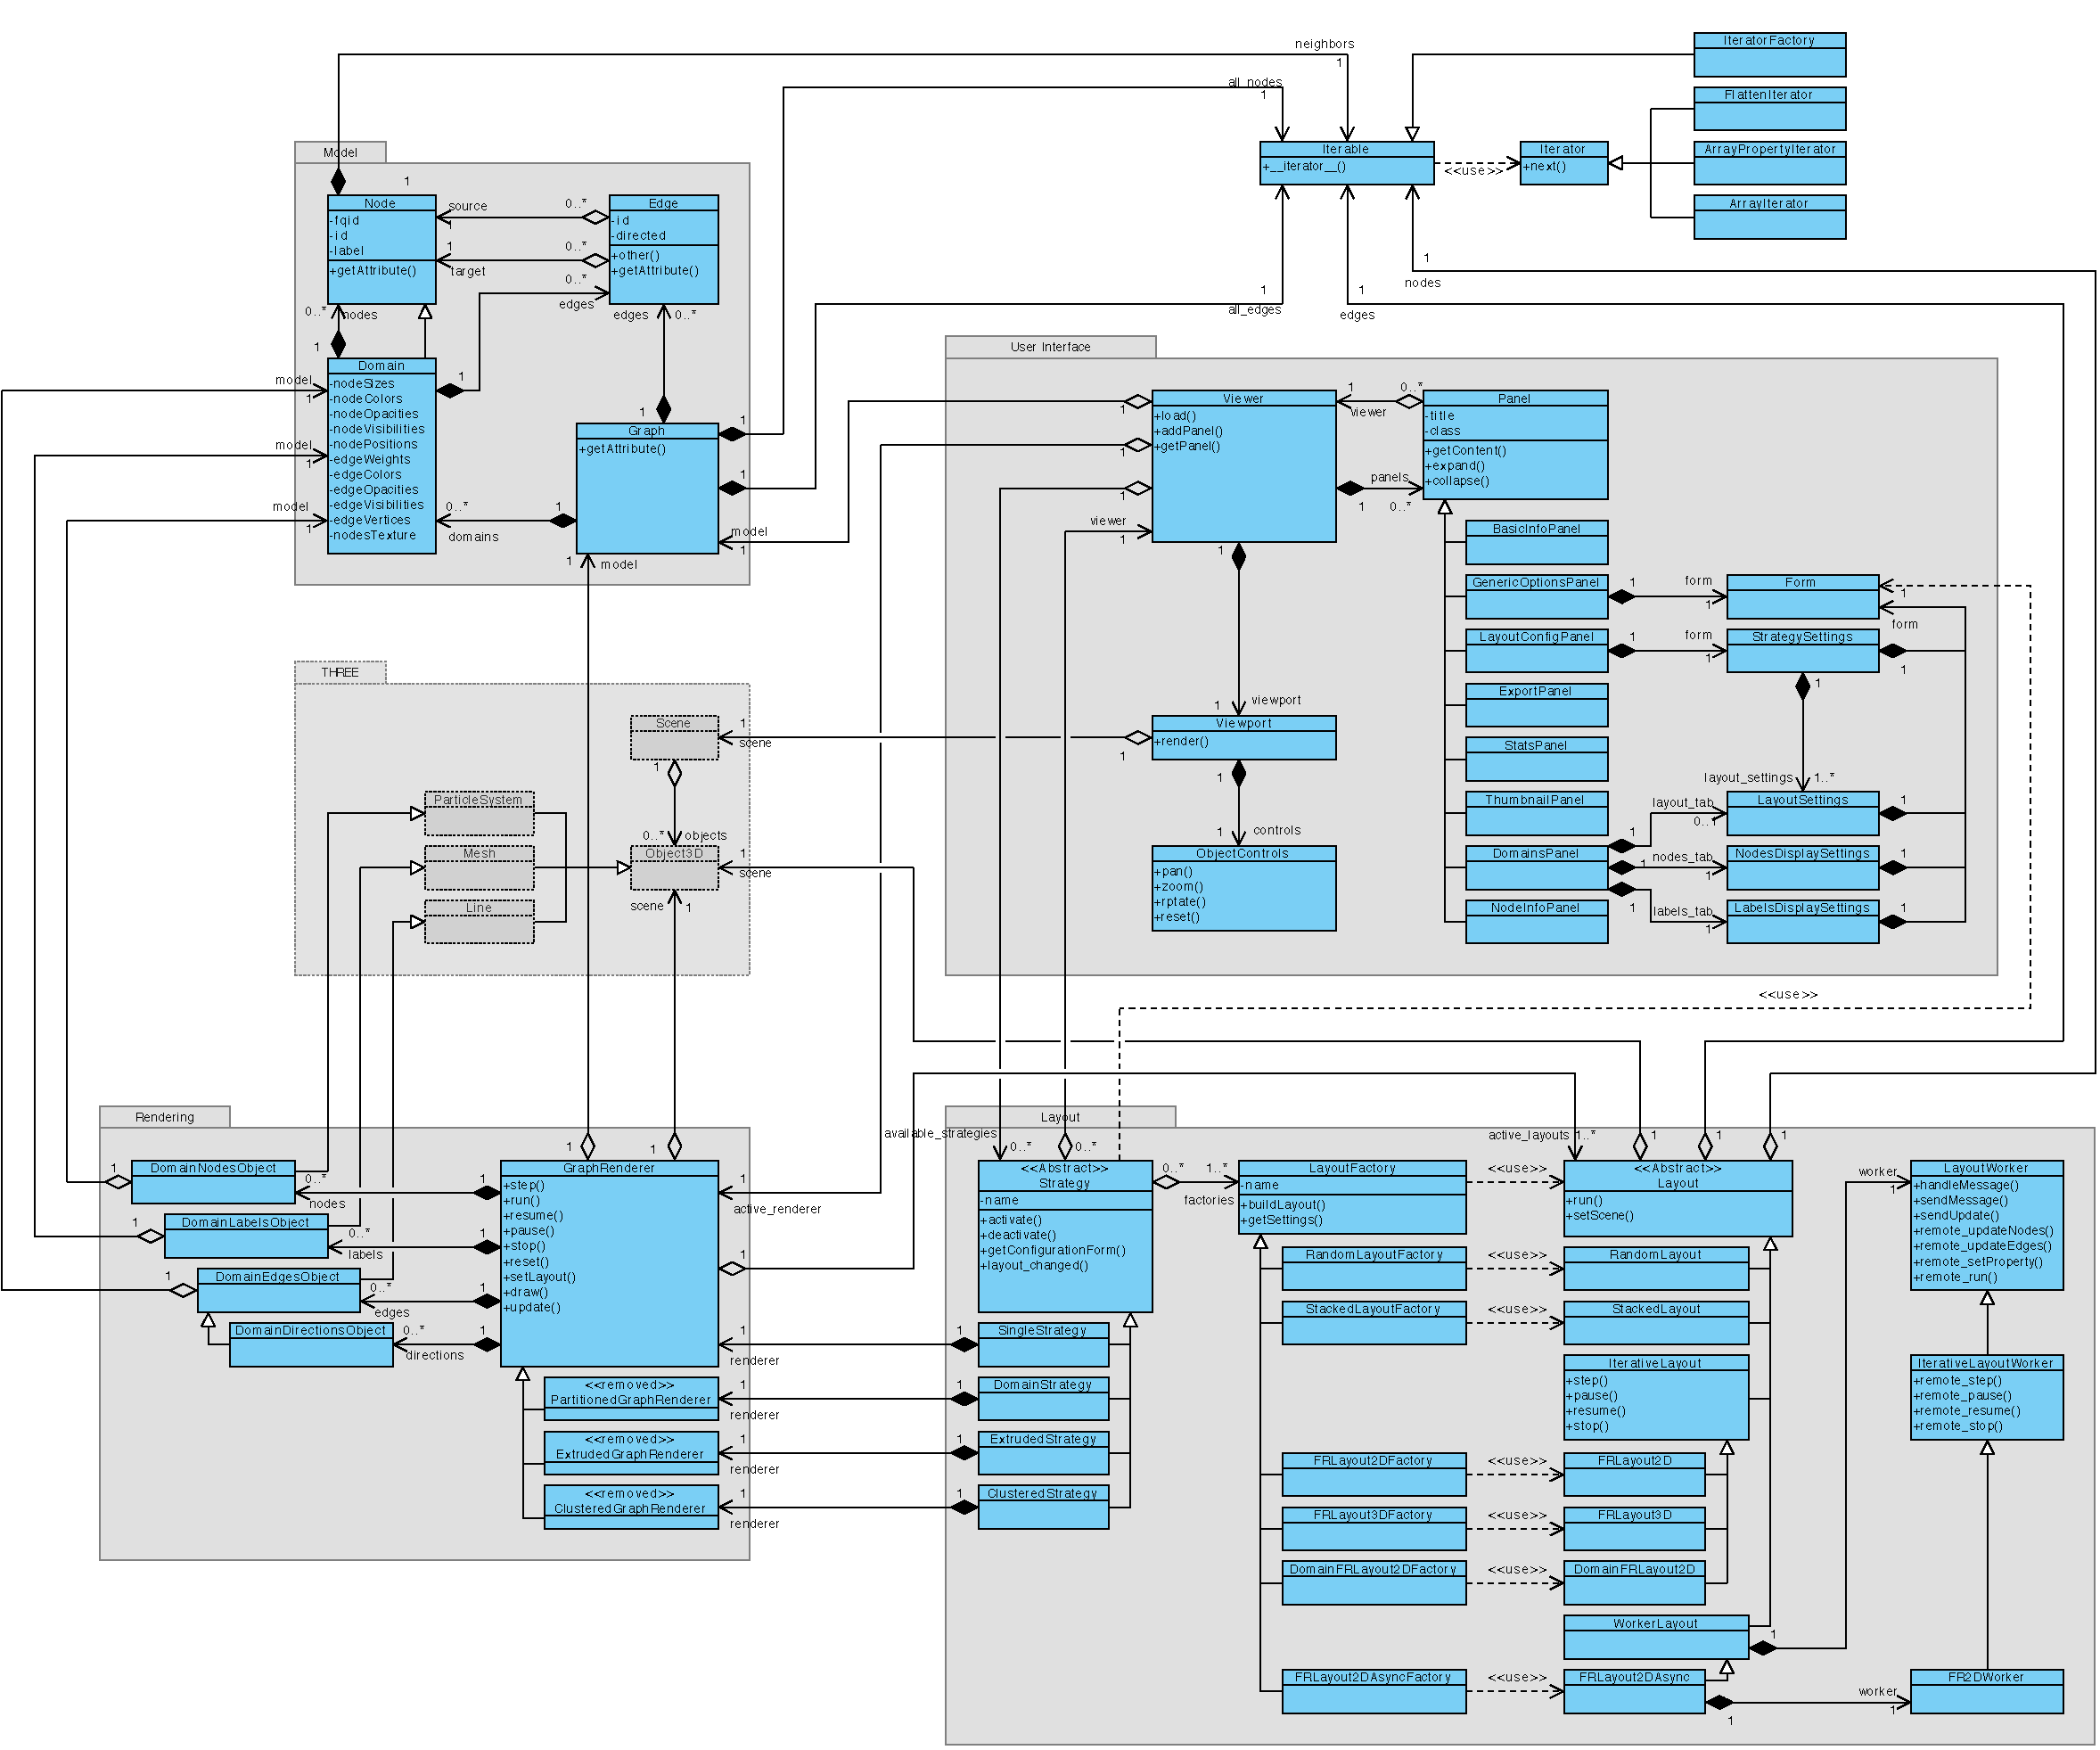
\includegraphics[height=1.05\textheight]{images/diagrams/class-visu}
    \caption[Class diagram for the whole graph visualization web application.]{Class diagram for the whole graph visualization web application, with the four core packages and fifth package to represent the external WebGL abstraction layer.}
    \label{fig:class-visu}
  \end{figure}
  \end{a3page}
}

\subsection{Overview}

\p{Introduction}
The whole system design is represented in the class diagram in \vref{fig:class-visu}. The diagram contains 5 packages, of which one represents the external library used as WebGL abstraction layer (the grayed out package named \emph{THREE}).

\p{Packages}
Of the four main packages, we present in detail the design of three of them: the \emph{Model}, \emph{Layout}, and \emph{Rendering} packages. The \emph{User Interface} package contains standard user interface glue code and is not as interesting as the other ones. The role played by the packages is best described as follows:

\begin{description}
  \item[Model] This package contains the classes to represent a multi-domain graph in memory, along with the utility methods to read its definition from a resource specifier and operate on it when using the other parts of the system. We discuss this package in detail in \vref{sec:visu/design/model}.
  \item[Layout] This package contains the framework used to lay out a multi-domain graph with the previously described \emph{strategy} and \emph{layout} model. The different implementations shipped with the application are also included in this package. We discuss it extensively in \vref{sec:visu/design/layout}.
  \item[Rendering] The role of this package is, given a graph model as input, to draw a representation of it. The default behavior is to draw a set of spheres connected by lines in \gls{3d} space, but other behaviors could be provided. The design of the \emph{Rendering} package is discussed in \vref{sec:visu/design/rendering}.
  \item[User Interface] As already anticipated, this package is responsible to build and maintain the user interface. It is responsible to provide the viewport to draw the graph and display the widgets that other components in the system need to accomplish their goal. We renounced to discuss the design of this package in the present report as it is very similar in structure to the one of other web applications.
\end{description}

\p{Pitfalls}
During the implementation of the presented design, different shortcomings where discovered, but an adequate solution could not be implemented on time. Similarly, in order to better adapt to the underlying WebGL infrastructure, we had to trade off some aspects of the design. In \vref{sec:visu/design/pitfalls} we discuss these findings in more detail.

\subsection{Graph model}
\label{sec:visu/design/model}

\p{Introduction}
This subsection focuses on how our application models a multi-domain graph. The relevant package is the \emph{Model} package in \vref{fig:class-visu}. The roles of the classes are self explanatory, we will thus focus here on more interesting aspects of their associations.

\p{Domains}
One of the first particularities is the \texttt{Domain} class inheriting from \texttt{Node}. For the purposes of our application, we consider a domain to be a \emph{top-level} node of a graph and nodes to be at the second level of the hierarchy, and thus contained in a domain. Seen in this way, the domains form a disjoint and complete partition of the nodes in a graph. Additionally, a \texttt{Domain} instance exposes different attributes used by the rendering engine. As inferable from their names, these attributes should belong to either the \texttt{Node} or the \texttt{Edge} instances. The reasons for this organization can be traced back to performance reasons and are better explained in \vref{sec:visu/design/pitfalls} and \vref{sec:visu/implementation}.

\p{Edges}
By partitioning nodes into domains, we now have two types of edges: \emph{intra}-domain edges within a domain and \emph{inter-}domain edges between nodes of different domains. The former are part of the enclosing \texttt{Domain} instance, while the latter are modeled as part of the main \texttt{Graph} instance. In both cases the edges can be accessed through the \texttt{edges} attribute.

\p{Iterators}
The last particularity regarding the graph model we discuss here regards the three associations with the \texttt{Iterable} class, namely \texttt{Node.neighbors}, \texttt{Graph.all\_nodes}, and \texttt{Graph.all\_edges}. In different places of the application we need to iterate over a list of all nodes (or edges) contained in a graph (e.g., an iterative layout working on the graph as a whole needs to iterate over all nodes and edges once for each step). As presented above, nodes and edges are scattered among the different domains of the graph and on the \texttt{Graph} instance itself, and creating an additional list for this purpose would present memory problems for larger graphs.\footnote{This problem propagates even further as other use cases that need to work on a particular selection of nodes or edges emerge and additional lists need to be created.} For these reasons we designed the \emph{iterator protocol} as a highly efficient way to expose any object as an iterable and used it to expose a collection of all nodes and edges in the graph. Additional details about iterators can be found in \vref{sec:visu/implementation/other}.


\subsection{Strategies and layouts}
\label{sec:visu/design/layout}

\p{Introduction}
The second package we focus on is the \emph{Layout} package. As anticipated in the overview, this package responsibility is, basically, given a graph model, to return a list of positions for each node contained in the network.

\p{Classes}
In the analysis we presented a model to lay out multi-domain graphs based on standard graph layout algorithms and strategies to apply them to multi-domain graphs. The natural result of this analysis is the creation of a \texttt{Strategy} and a \texttt{Layout} class. To completely cover all the required functionality, we need at least an additional class: the \texttt{LayoutFactory}. As the name suggests, this class is responsible to create new \texttt{Layout} instances when needed.

\p{Strategies}
Each concrete \texttt{Strategy} subclass owns both a list of layout factories to use to create the layout algorithms it needs and a reference to a \texttt{GraphRenderer} which takes care of running the algorithms and drawing the graph. The four \texttt{Strategy} subclasses shown in the diagram contain the implementation of the four strategies presented in \vref{sec:visu/results}.

\begin{figure}
  \begin{adjustwidth}{-4.65mm}{-5.7mm}  
    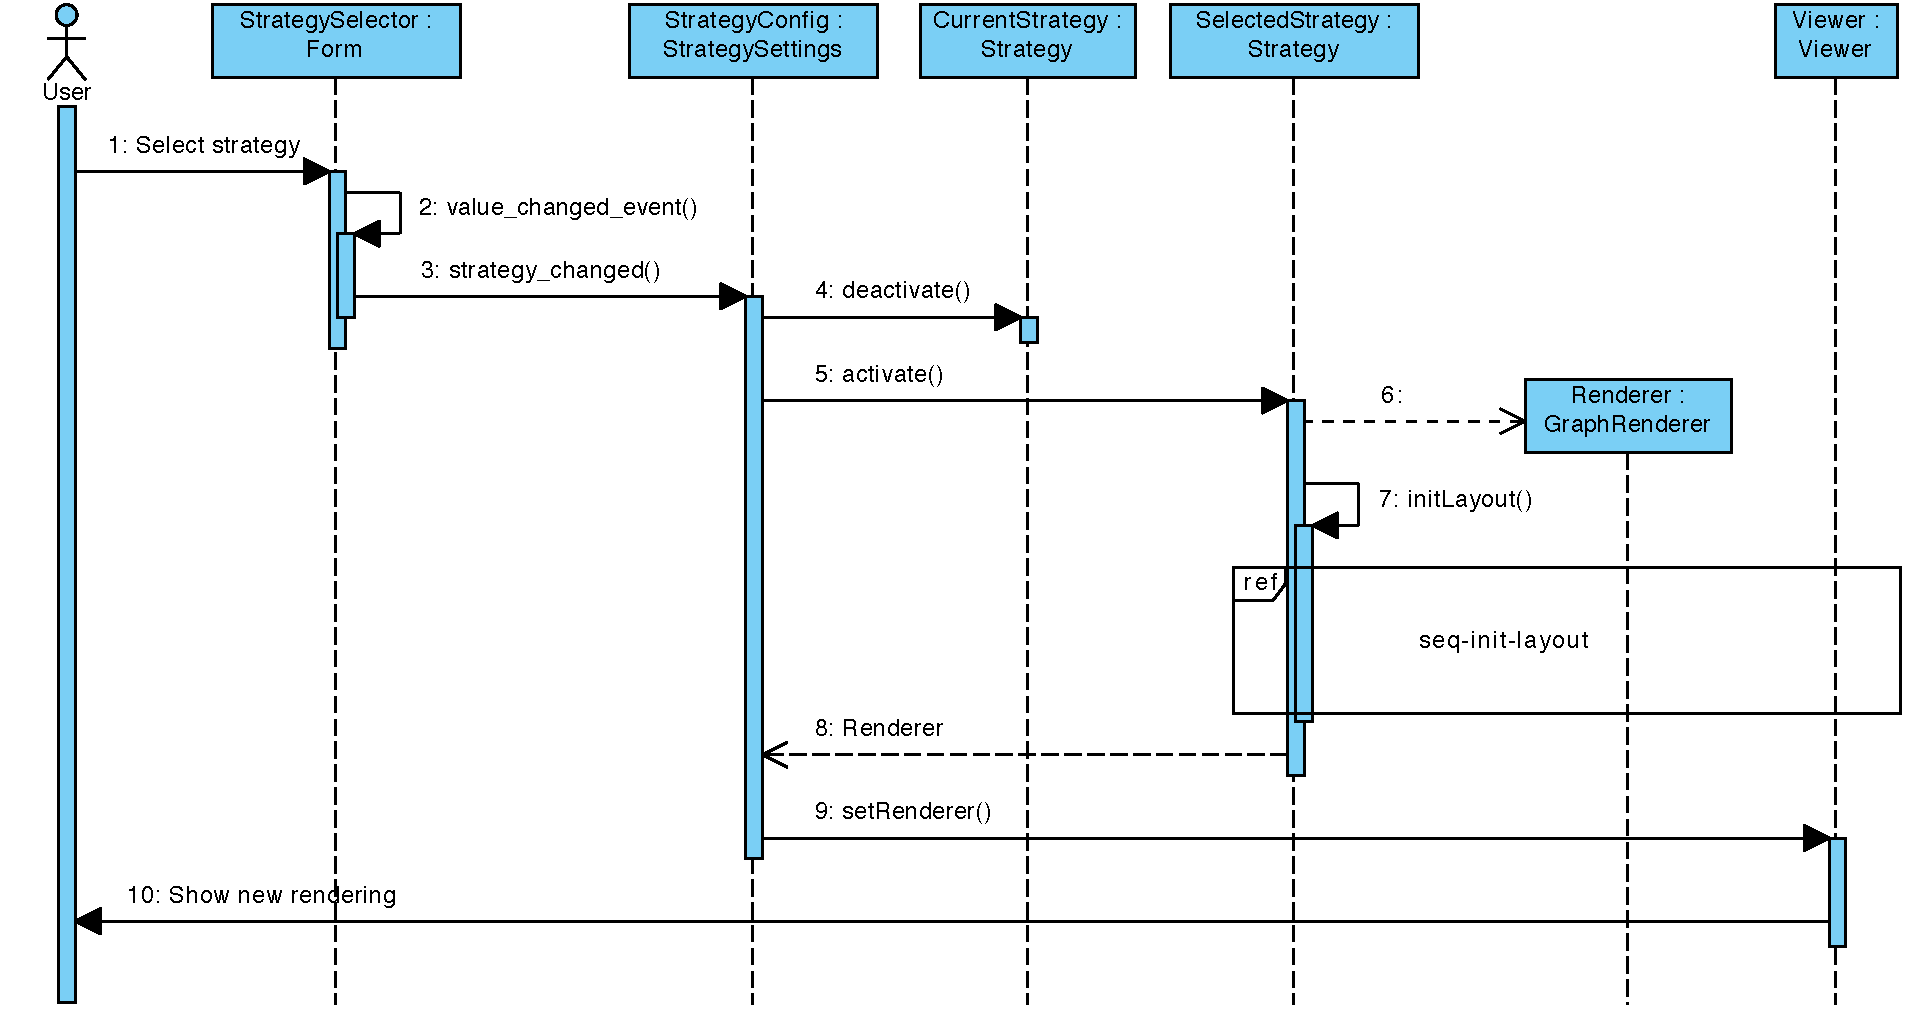
\includegraphics[width=\linewidth]{images/diagrams/seq-strategy}
  \end{adjustwidth}
  \caption[Sequence diagram for the strategy selection process.]{Sequence diagram showing the different steps involved in selecting a new strategy. The referenced \texttt{seq-init-layout} diagram is shown in \vref{fig:seq-init-layout}.}
  \label{fig:seq-strategy}
\end{figure}

\p{Strategy selection}
The sequence diagram in \vref{fig:seq-strategy} shows the steps involved in the selection of a new strategy when the user triggers the process by selecting it from a drop down in the user interface. As visible in the diagram, \texttt{Strategy} instances are never destroyed, but switched between by means of their \texttt{activate} and \texttt{deactivate} methods (messages 4 and 5). Additional details about the initialization of the layout algorithms is provided in the subdiagram in \vref{fig:seq-init-layout}.

\p{Layout}
A \texttt{Layout} instance is responsible to lay out nodes in a \gls{2d} or \gls{3d} space. In the normal case, it simply implements a well-known layout algorithm. In order to fulfill its task, the instance needs a reference to a list of nodes and a list of edges. This information is passed as an iterator, as already explained for the graph model in \vref{sec:visu/design/model}. In this case, through the use of custom iterators, more complex setups can be achieved in a memory efficient way. The third association shown in the class diagram refers to a \texttt{Object3D} instance. The layout algorithm can use this object to draw additional elements on the final viewport. For example, in the included Fruchterman-Reingold \gls{2d} implementation, we use it to draw the plane on which the nodes are laid out.

\p{Layout selection}
The selection of a new layout algorithm to use as building block for a strategy can be carried out by the user in a similar way as done for the strategy in the previous paragraphs. The context for this process is illustrated in the sequence diagram in \vref{fig:seq-layout}, while more details are provided in the already referenced subdiagram in \vref{fig:seq-init-layout}, and described in the next paragraphs. The main difference with regard to the selection of a new strategy is that the current layout instance is destroyed and a new one created by means of a \texttt{LayoutFactory}.

\begin{figure}
  \begin{adjustwidth}{-5.2mm}{-6.5mm}  
    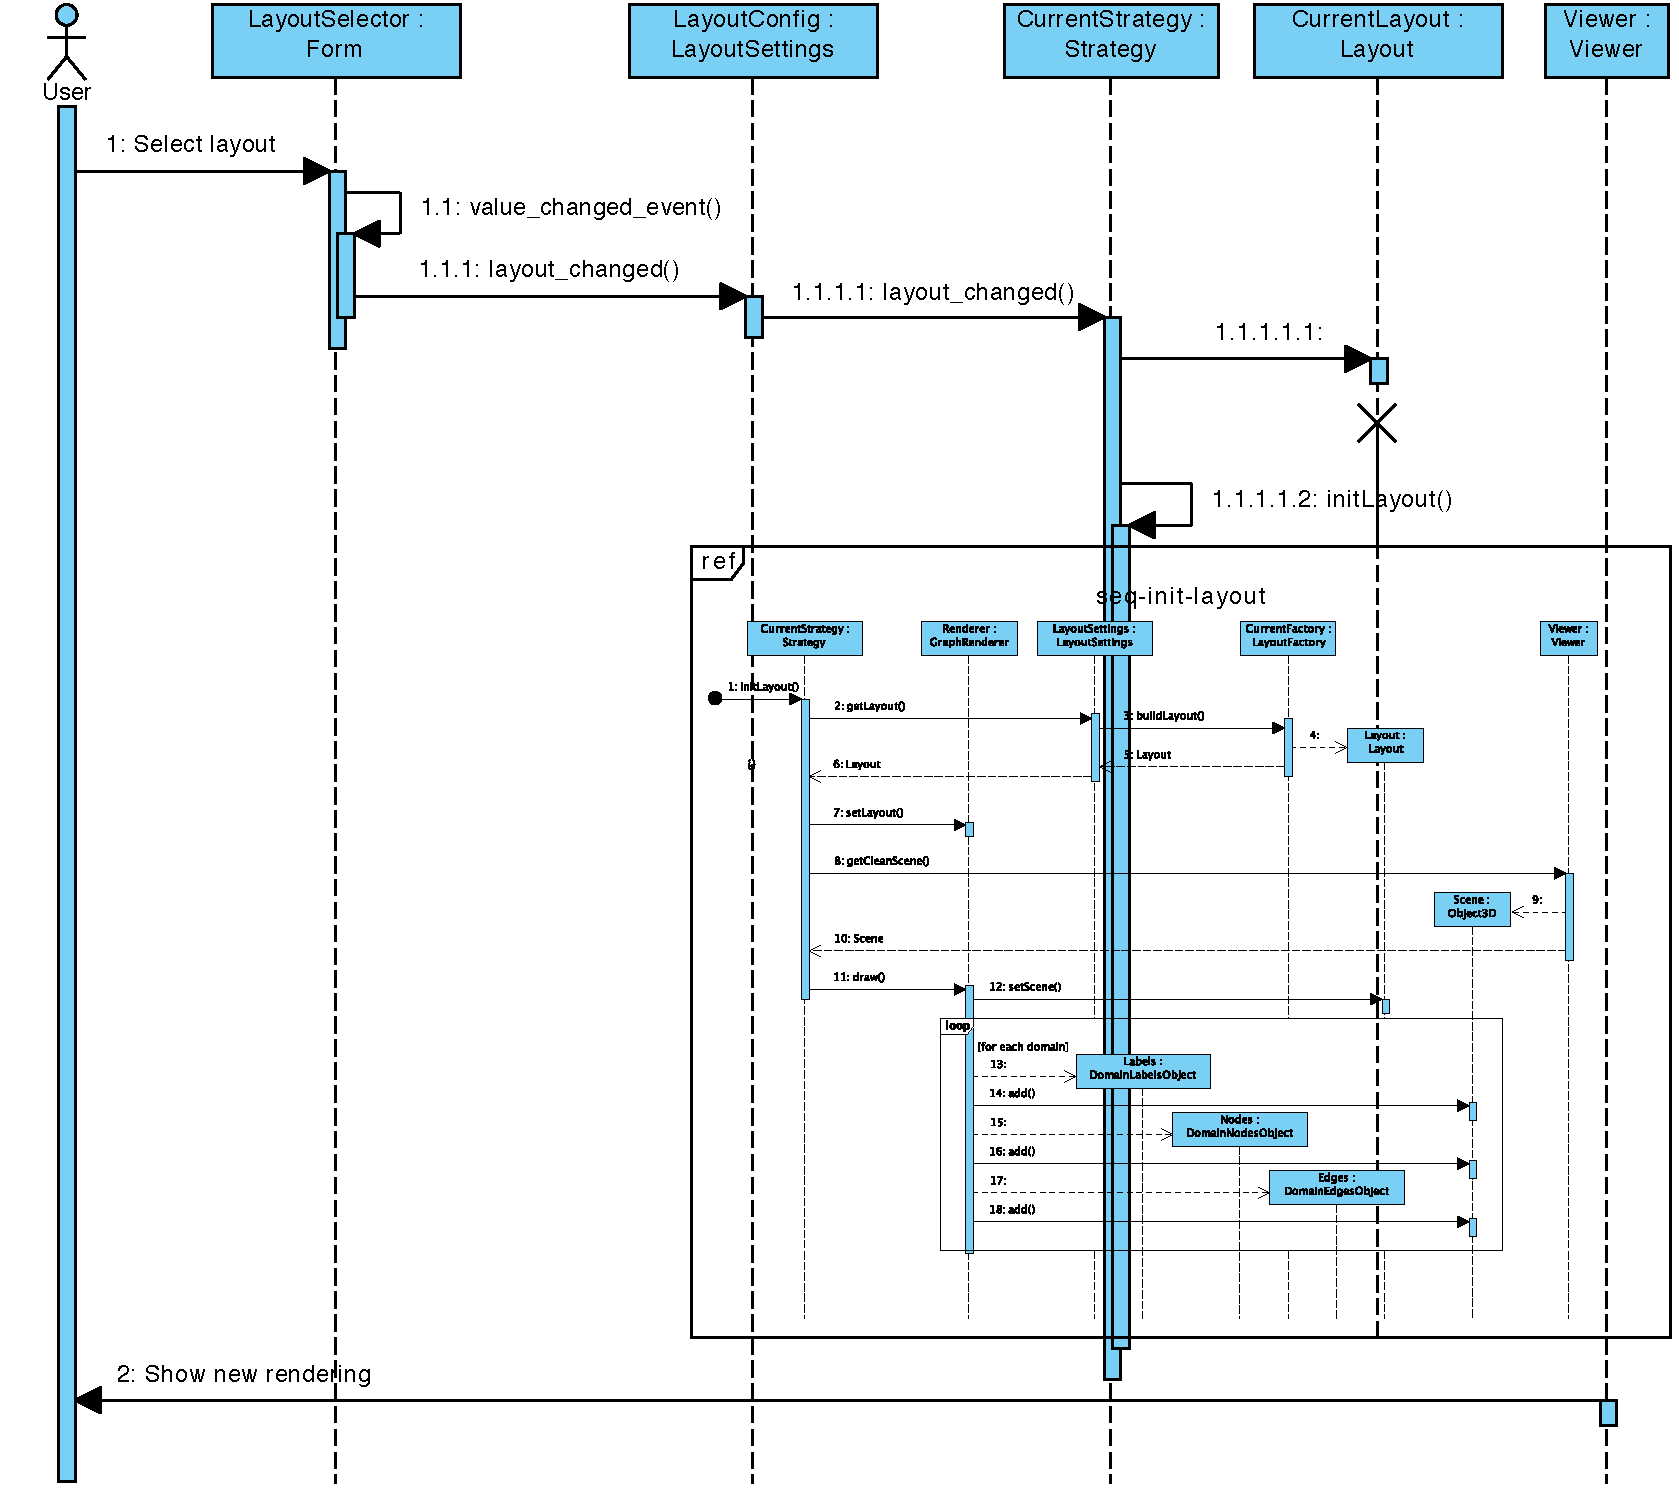
\includegraphics[width=\linewidth]{images/diagrams/seq-layout}
  \end{adjustwidth}
    \caption[Sequence diagram for the layout selection process.]{Sequence diagram showing the different steps involved in selecting a new layout algorithm. The referenced \texttt{seq-init-layout} diagram is shown in \vref{fig:seq-init-layout}..}
  \label{fig:seq-layout}
\end{figure}

\p{Layout factory}
The association of a strategy with its supported layouts is carried out by the means of \texttt{Layout\BreakableSlash{}Factory} instances. By using the factory pattern, we abstract the differences between the different \texttt{Layout} implementations away from the strategy itself. Each layout implementation has to provide its own factory. A \texttt{LayoutFactory} instance has two main methods:

\begin{description}
  \item[\texttt{getSettings}] is responsible to return a list of configuration options which are used by the user interface code to build a \texttt{Form} instance. Each option has to provide at least a name and a type for the data the user can configure.
  \item[\texttt{buildLayout}] is used by the encapsulating strategy to create a new \texttt{Layout} instance. Once the instance is created, the user-configured settings can be passed to it.
\end{description}

\p{Creation of a new \texttt{Layout} instance}
The usage of the \texttt{LayoutFactory} instance to create a new layout algorithm implementation is illustrated in the sequence diagram in \vref{fig:seq-init-layout}, referenced by both the strategy selection and the layout selection processes. Beside the obvious factory pattern (messages 2 through 6), the sequence diagram shows how a new scene is constructed each time the layout algorithm is changed: first by discarding the current scene and getting a new one (messages 8 to 10) and then by redrawing the whole graph (messages 11 and following). Additional details about the rendering process are discussed in the next subsection.

\begin{figure}
  \begin{adjustwidth}{-18mm}{-6.2mm}  
    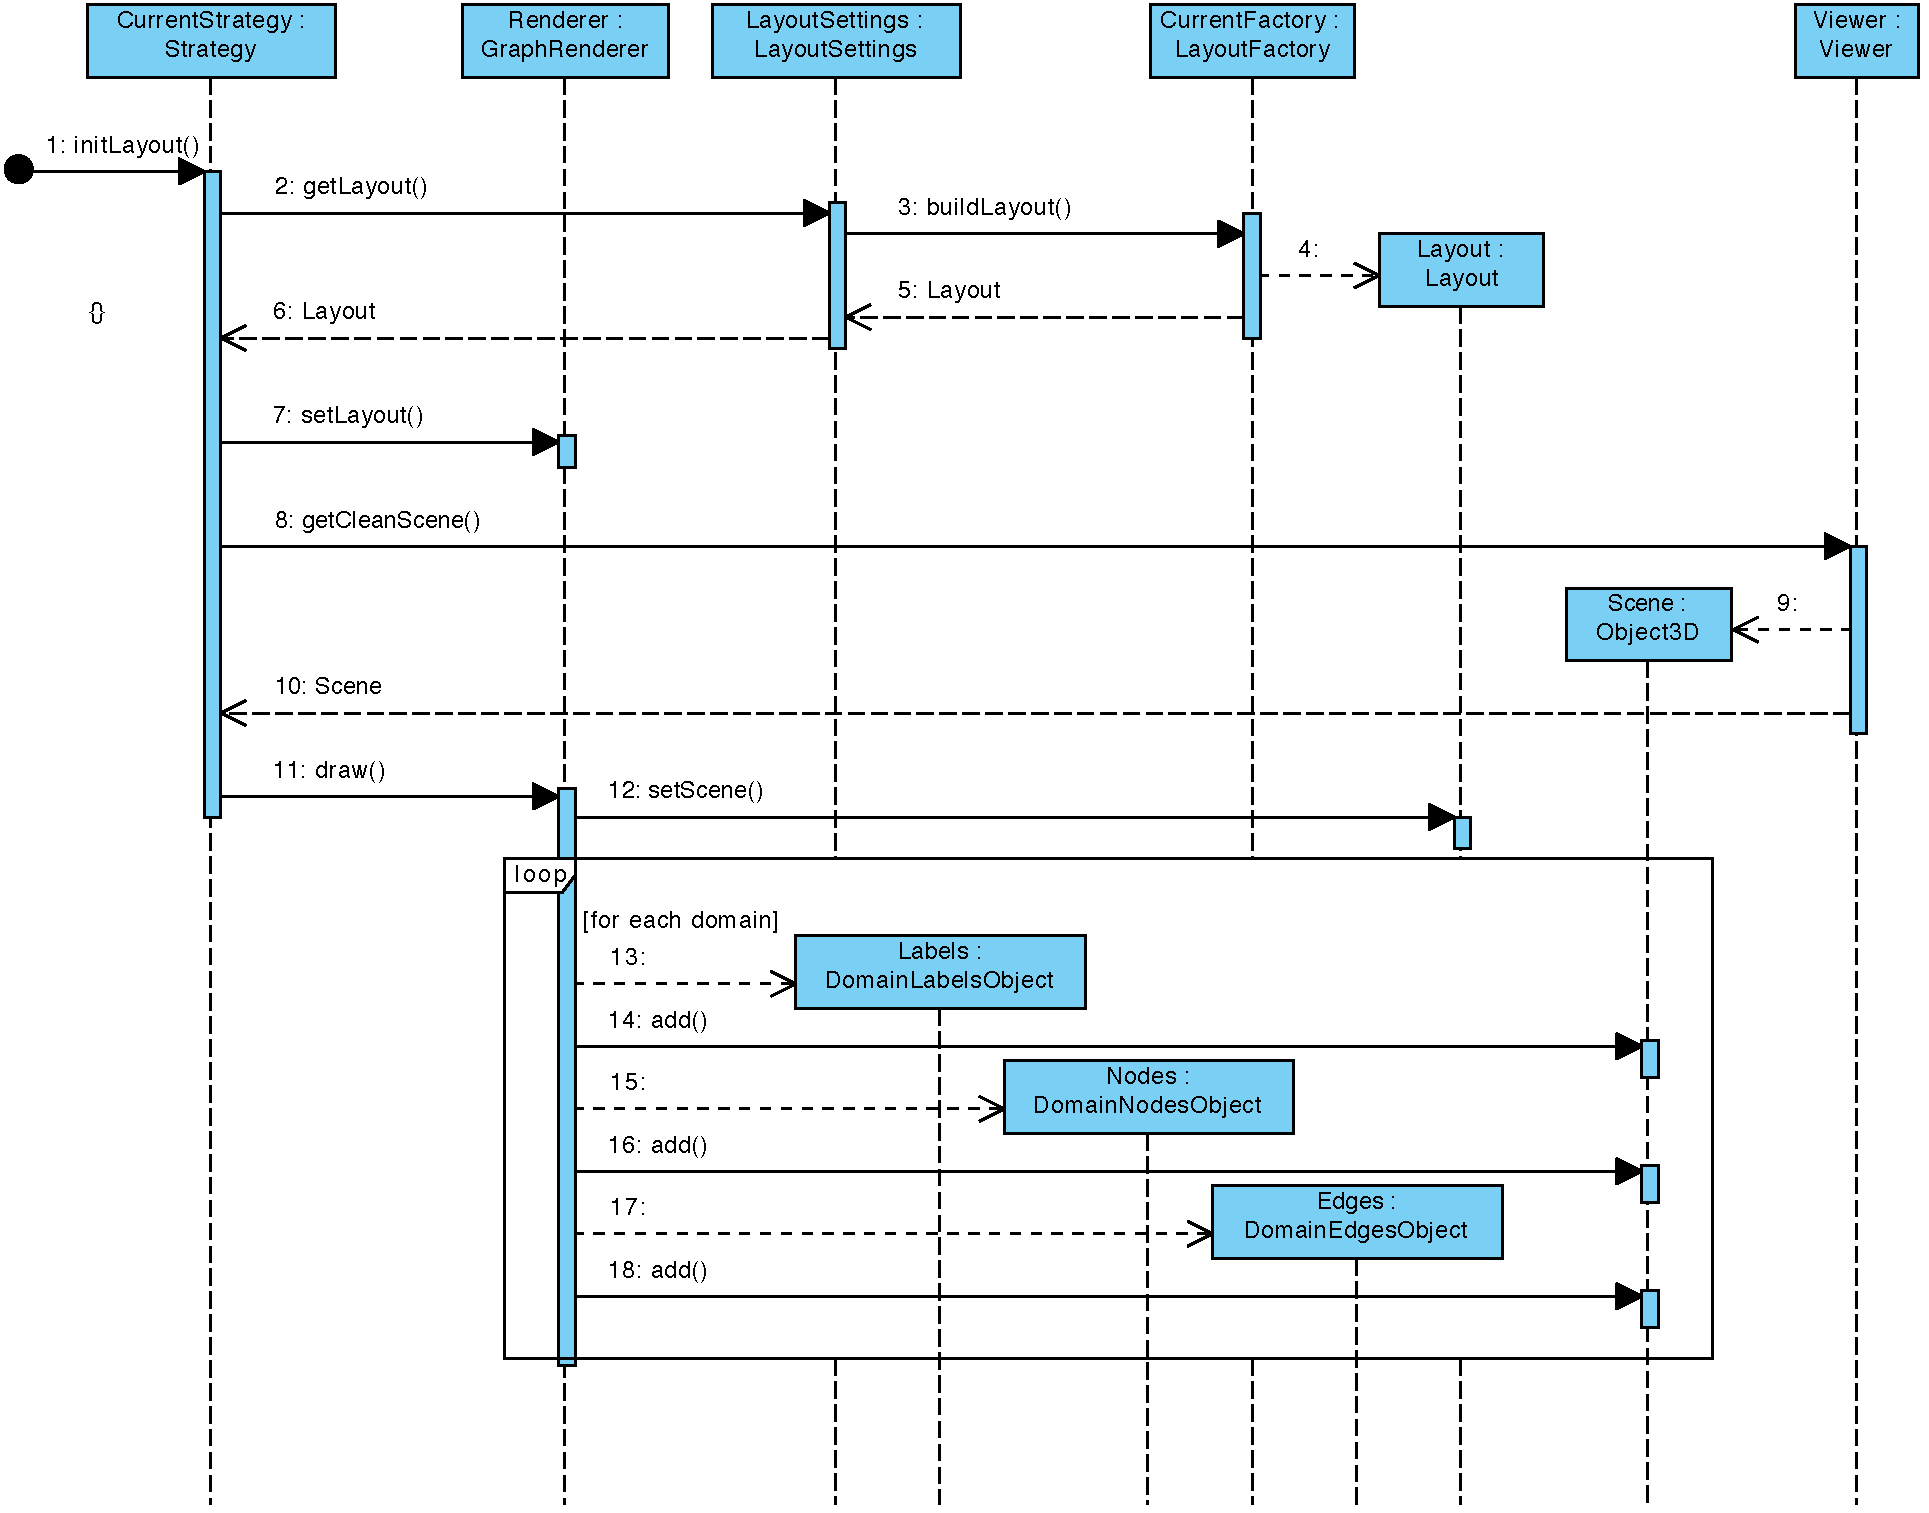
\includegraphics[width=\linewidth]{images/diagrams/seq-init-layout}
  \end{adjustwidth}
  \caption[Sequence diagram for the initialization of a new layout algorithm.]{Sequence diagram for the initialization of a new layout algorithm. This diagram is referenced in \ref{fig:seq-strategy} and \ref{fig:seq-layout}. as \texttt{seq-init-layout}}
  \label{fig:seq-init-layout}
\end{figure}

\p{Iterative layouts}
Different layout algorithms are based on a series of iterations to incrementally optimize the layout of the graph. As implementations of this kind share most of the bookkeeping code, a specialized subclass is provided in the form of \texttt{IterativeLayout}. A minimal implementation of an iterative layout has thus to implement just the \texttt{step} method, while all the aspects of the iteration are taken care of by the superclass.

\p{Asynchronous layouts}
In order to implement asynchronous layouts running in a web worker\footnote{A \emph{web worker} is similar to a thread in a normal process, without context sharing and supporting only message passing as communication facility.} \cite{webworker}, an additional \texttt{Layout} specialization is provided by the \texttt{WorkerLayout} subclass. This subclass communicates with a ``remote'' layout implementation through the interface provided by the \texttt{LayoutWorker} class. In addition to the message passing facilities, this class also implements the basic layout execution code for the asynchronous environment. The \texttt{IterativeLayoutWorker} subclass provides the specialized code to support iterative layouts in the asynchronous environment as done by \texttt{Iterativelayout} for the sequential implementation.

\p{Layout execution}
\Vref*{fig:seq-execute-layout} shows the sequence diagram for the execution of a strategy making use of an asynchronous layout algorithm. It is important to note that the control flow is released (and thus made available for other user-interface related actions) with message 11. All the following operations, including the calculation of the node positions, happen asynchronously in the web worker. 

\begin{figure}[t]
  \begin{adjustwidth}{-4.6mm}{-2.5cm}  
  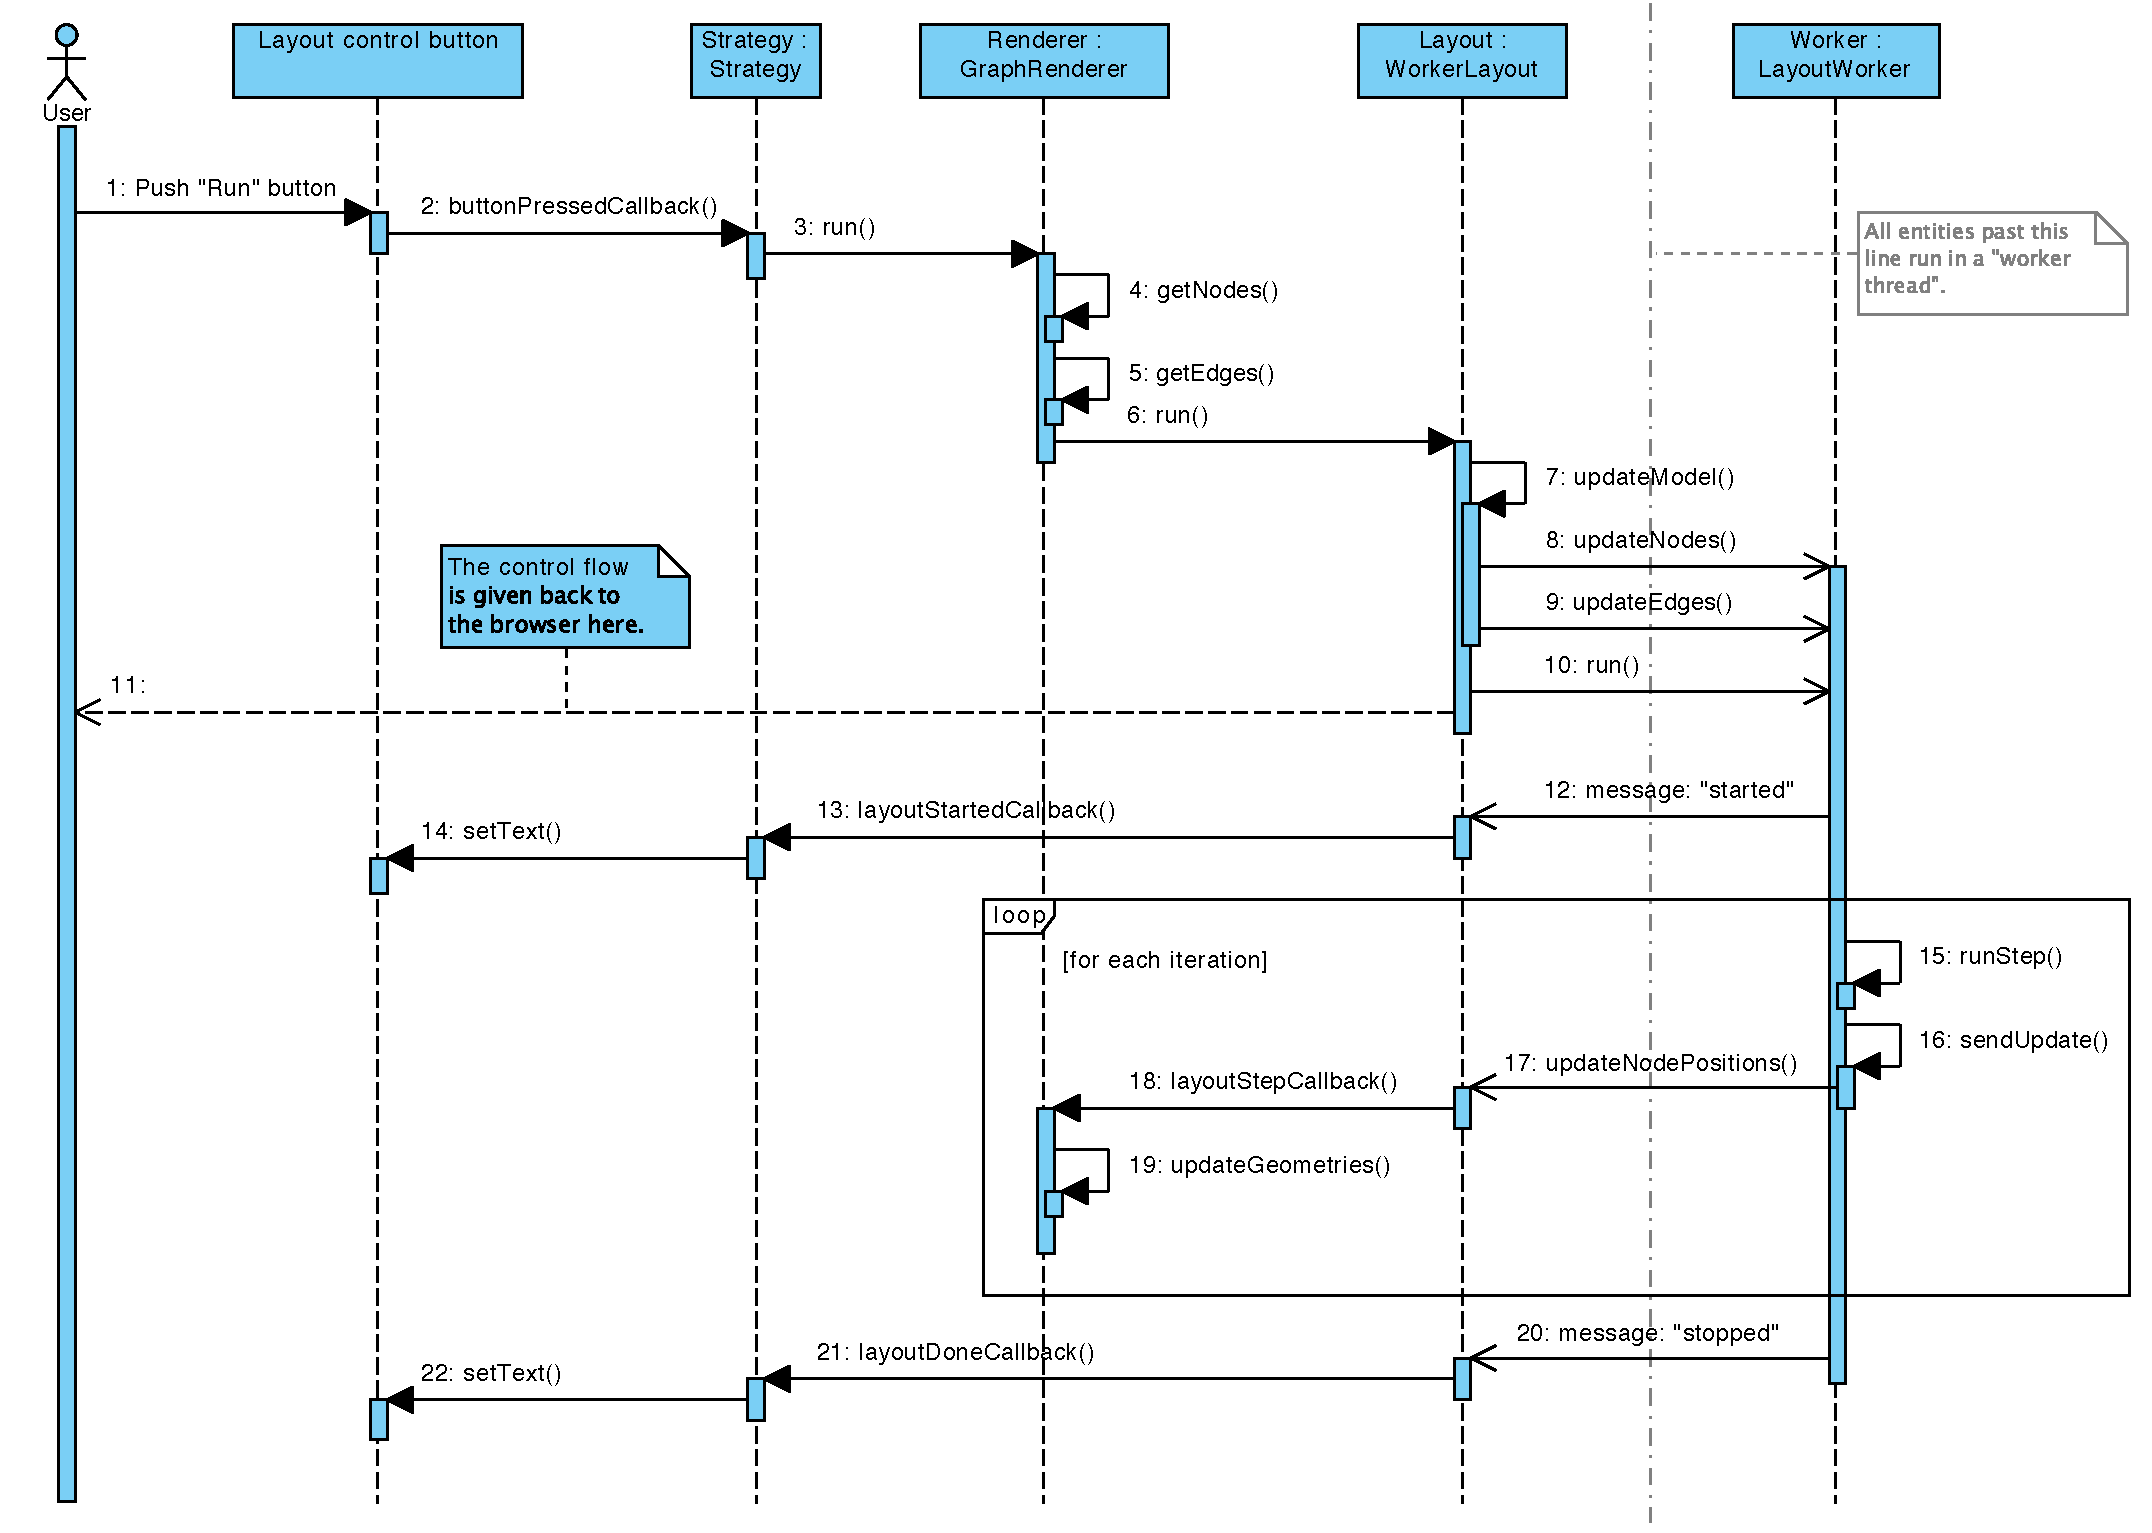
\includegraphics[width=\linewidth]{images/diagrams/seq-execute-layout}
\end{adjustwidth}
  \caption[Sequence diagram for the execution of an asynchronous layout.]{Sequence diagram for the execution of an asynchronous layout algorithm.}
  \label{fig:seq-execute-layout}
\end{figure}

\p{Advantages}
There are two main advantages obtained by deferring the layout computation to a separate worker which directly impact the user experience:

\begin{enumerate}
  \item The computation does not happen in the same thread running the user interface code. It can thus not block the user interface during the computation. This problem has partially been solved for synchronous layouts by using deferred events.
  \item Strategies using multiple layout algorithms can now defer each algorithm to a different web worker and can thus parallelize their execution.
\end{enumerate}

Additionally, the \emph{nothing-shared} web worker architecture made necessary the use of message passing techniques for inter-worker communication. The advantages are twofold in this case as well:

\begin{enumerate}
  \item Low level synchronization problems are mitigated as no worker can modify an in-memory value used by another worker.
  \item The same interfaces can be used to implement a \emph{remote} version of the \texttt{LayoutWorker} class, running on a different host and possibly in a different environment (e.g., a layout algorithm written in C and taking advantage of multiple processors).
\end{enumerate}

\subsection{Graph rendering}
\label{sec:visu/design/rendering}

\p{Overview}
The last package we discuss is the \emph{Rendering} package. We offer just an overview in this subsection, preferring to add more details about its implementation in the next one (\vref*{sec:visu/implementation}). The \emph{Rendering} package responsibility is to execute the layout algorithms with the setup defined by the strategy and draw the result as an \texttt{Object3D} object which gets added to the visualized scene.

\p{Classes}
To achieve its goals, the \emph{Rendering} package consists of two types of classes:
\begin{description}
  \item[\texttt{GraphUpdater}] and its subclasses are responsible to create the different objects to render the graph and to run the layout algorithms.
  \item[\texttt{Domain<type>Object}] classes where \texttt{<type>} stands for either \texttt{Nodes}, \texttt{Labels}, \texttt{Edges}, or \texttt{Directions}, are actual \texttt{Object3D} subclasses and are responsible for the \gls{3d} representation and the drawing of the different objects to the screen. More details about this particular design, instead of for example, a \texttt{Node} object for each node, are discussed in \vref{sec:visu/implementation}.
\end{description}

\subsection{Pitfalls in the current design}
\label{sec:visu/design/pitfalls}

\p{Introduction}
The design presented in this section accurately describes the implemented code. However, during the implementation, we discovered different possible optimizations. For lack of time, and for the purposes of the prototype, we did not adapt the design to these findings. In this subsection we briefly discuss these possible improvements.

\p{Renderers and strategies}
The first flaw in the design, also clearly visible in the class diagram, is the proliferation of classes in the \emph{Rendering} package due to \texttt{Strategy} subclasses in the \emph{Layout} package. This behavior derives from a wrong separation of concerns between \texttt{GraphRenderers} and \texttt{Strategies}. In the previous subsection, we described a graph renderer as having two roles: running the layout algorithms and rendering the graph. While the latter one is correct, the former should really be a task of the \texttt{Strategy} instance.

\p{Strategy factories}
An additional design problem in the same set of classes is keeping \texttt{Strategy} objects around even when they are not active (cf. \vref{fig:seq-strategy}). The design, and the implementation would be more intuitive by applying the factory pattern to the strategies as well, in a similar way as done for the layout algorithms. A new class diagram containing only the interested classes is shown in \vref{fig:class-visu-ok}. Classes with a green background belong to the newly introduced factory pattern for strategies; classes in orange represent the modified classes, while classes with a red background where completely removed from the design.

\begin{figure}
  \begin{adjustwidth}{-2mm}{-0.8mm} 
    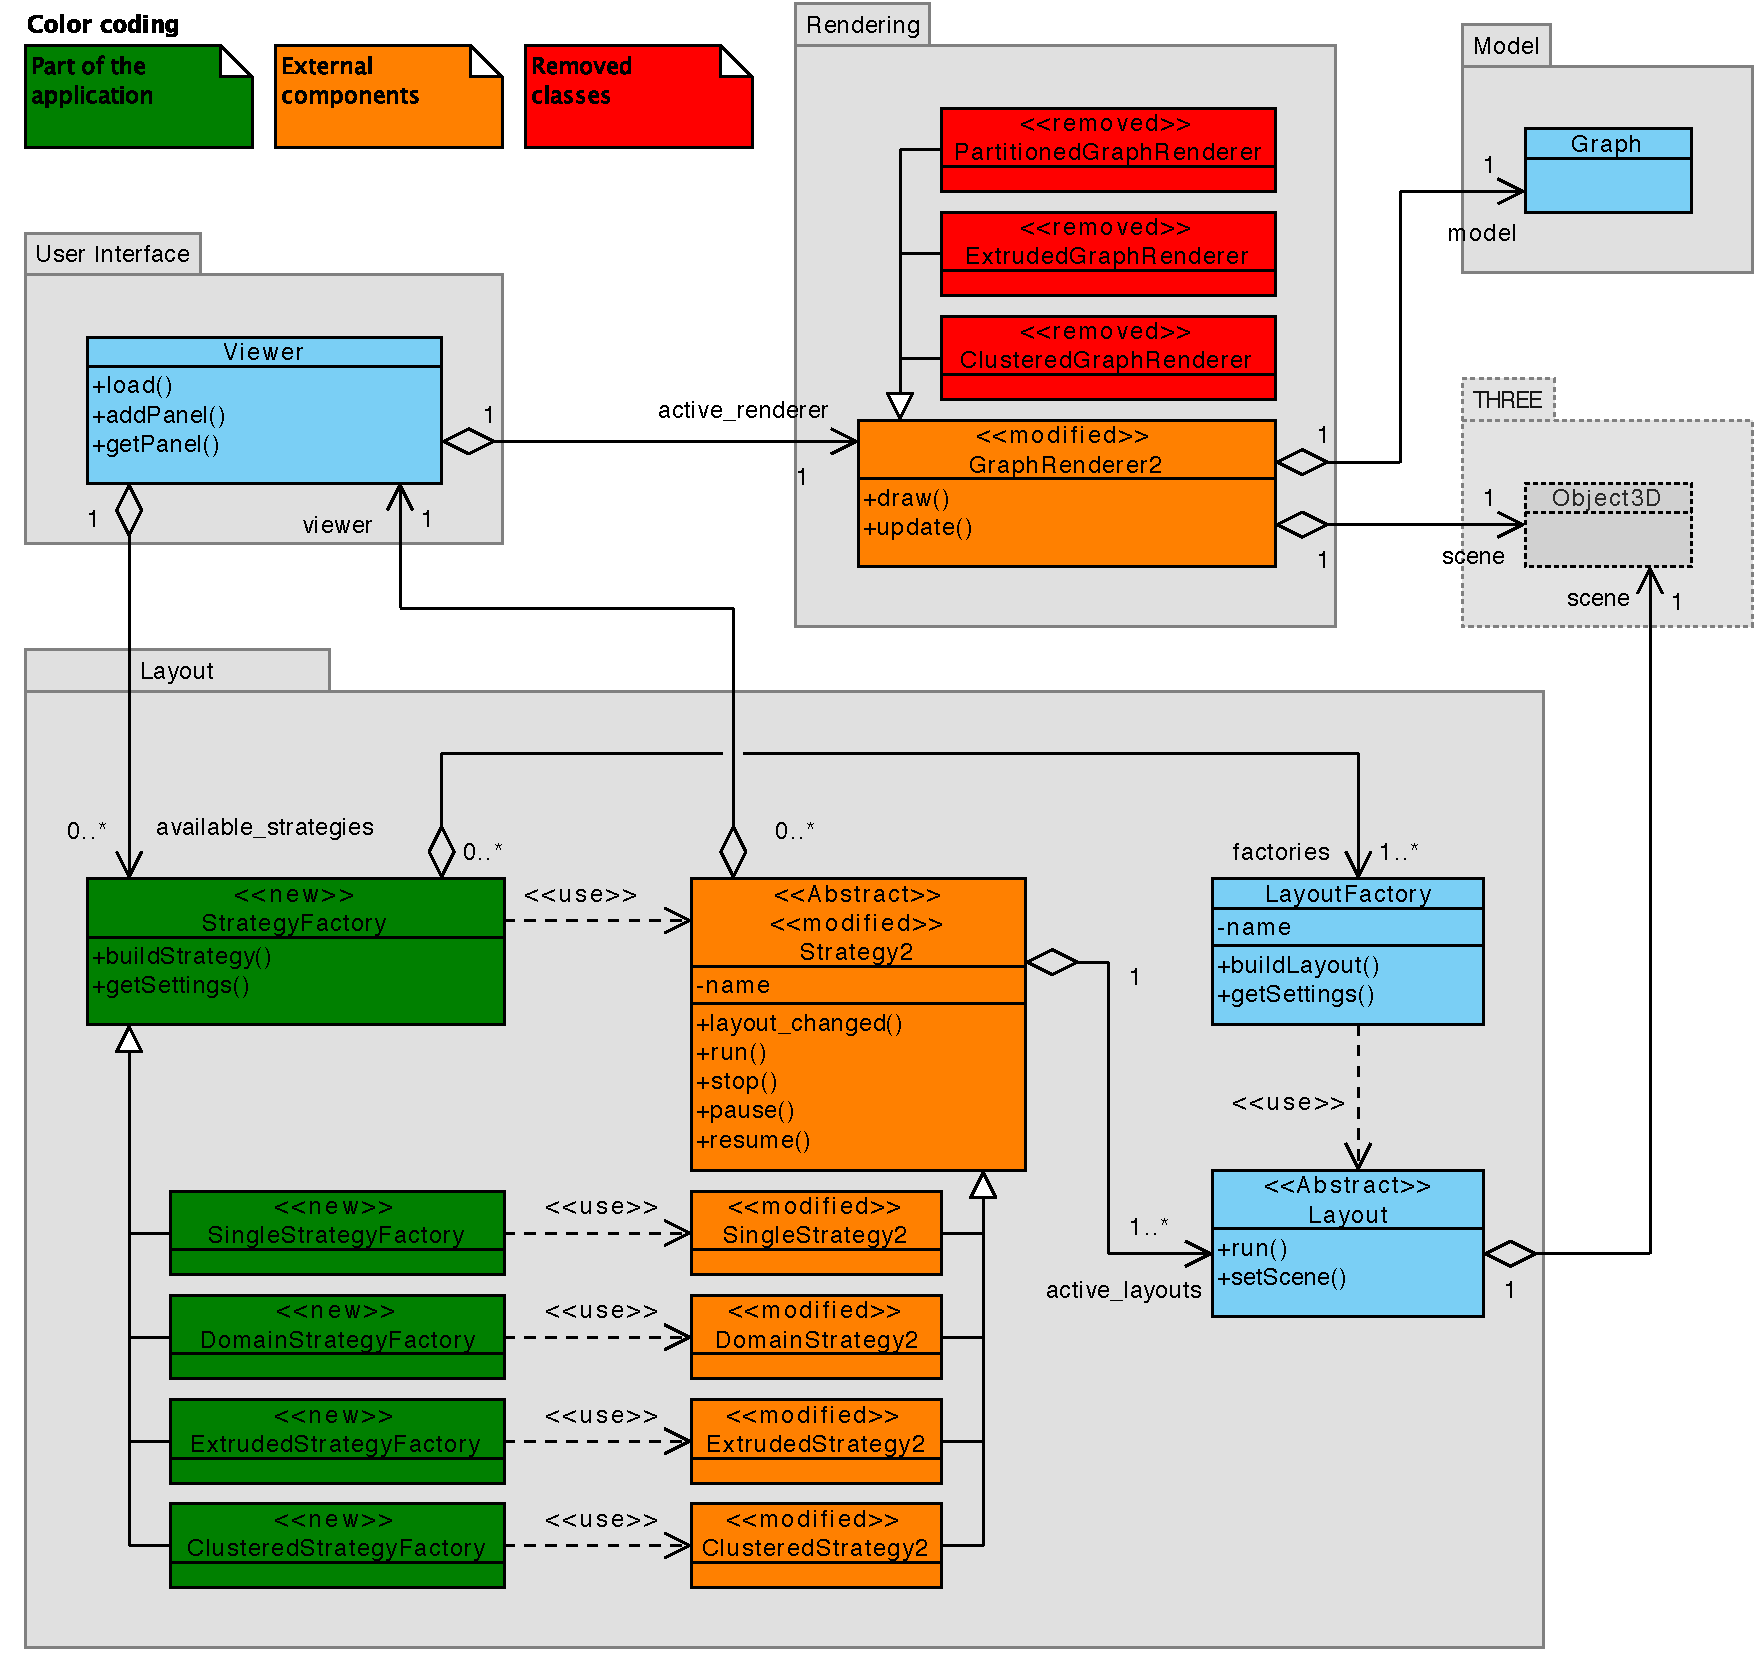
\includegraphics[width=\linewidth]{images/diagrams/class-visu-ok}
  \end{adjustwidth}
  \caption[Amended class diagram with changes highlighted.]{Class diagram amended with the considerations regarding the discovered pitfalls in the implemented design.}
  \label{fig:class-visu-ok}
\end{figure}

\p{Event dispatching}
A pitfall not visible in the class diagram concerns the management of events. During the usage of the applications, many components need event handling capabilities (e.g., \emph{layout started}, \emph{graph loaded}, etc.). By not having explicitly included support for event management in the design, we ended up implementing custom event handling over and over again for each class needing it. A better solution would be to include a generalized observer pattern in the design and make the relevant classes use it.

\p{Implementation-dictated design choices}
Two non-obvious design choices are dictated by implementation details of the underlying WebGL abstraction wrapper. The first one is the modeling of the graph as a \gls{3d} object by using containers instead of single objects. For example, the nodes are modeled in \gls{3d} by the \texttt{DomaniNodesObject} class rendering all the nodes in a given domain. Design-wise, a better approach would be to model each single node with a \texttt{NodeObject} instance. We originally designed the system this way, but for performance reasons illustrated in the next chapter, we had to switch to the current design. The proliferation of node- and edge-specific properties on the \texttt{Domain} object (e.g., \texttt{nodePositions}, \texttt{edgeColors}, etc.) stems from exactly the same issue and is discussed in the next chapter as well.


\section{Implementation}
\label{sec:visu/implementation}

\p{Introduction}
In this section we present the particularities emerged during the implementation of the previously discussed design. As the most interesting challenge emerged during the implementation was to keep the performances at an acceptable level, the discussions will mainly focus on two aspects where performance played an important role: the graph rendering engine, and the asynchronous layout execution.

\subsection{Efficient nodes drawing}

\p{High CPU usage}
The first problem encountered when drawing graphs of an important size ($|V| > 2000$, in our case) was that even when the application was not doing anything, the \gls{cpu} usage never fell below a certain threshold. By profiling the application, we discovered that the underlying \gls{3d} rendering engine tries to render 60 frames per second. This is not a problem by itself, as many animations need to run at a high frame rate to provide a fluid experience. The problem laid in the high number of objects that had to be drawn at each iteration.

\p{Drawing calls}
The first prototype of the graph rendering engine drew a sphere for each node in the graph. This meant that for each frame, the JavaScript code had to call a WebGL function for each node in the graph. As this approach did not scale, we were forced to adapt the design and use a \texttt{ParticleSystem} object instead, a special kind of \gls{3d} object optimized to draw a large amount of \emph{particles} in a \gls{3d} space. The difference between the two modes of operation are shown in the sequence diagrams in \vref{fig:node-draw}.

\begin{figure}
  \begin{adjustwidth}{-1.4mm}{-2.2mm}
    \subfloat[Expensive drawing]{%
      \label{fig:expensive}%
      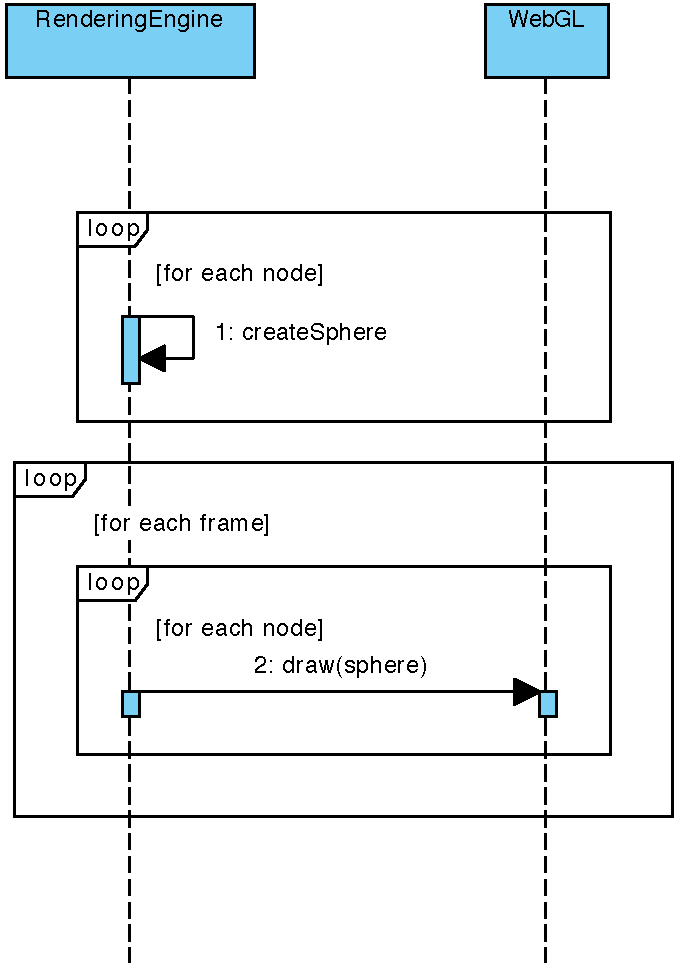
\includegraphics[height=9.2cm]{images/diagrams/seq-draw-expensive}%
    }%
    \hfill
    \subfloat[Inexpensive drawing]{%
      \label{fig:inexpensive}%
      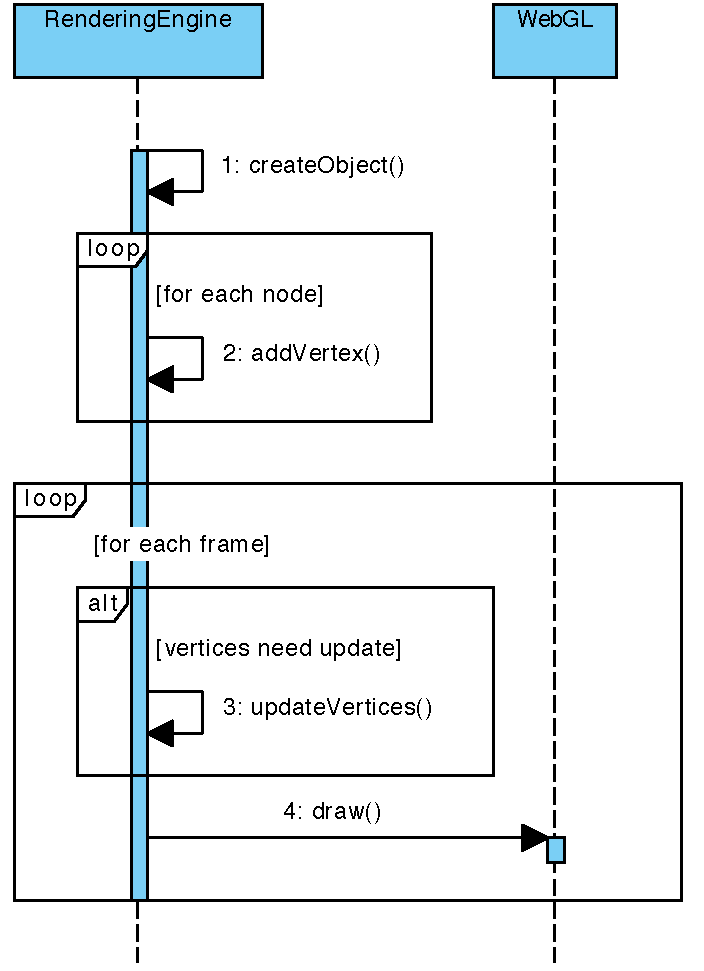
\includegraphics[height=9.2cm]{images/diagrams/seq-draw-inexpensive}%
    }
  \end{adjustwidth}
  \caption[Two different approaches to render a large number of nodes.]{Two approaches having a different impact on performance when drawing a large number of nodes.}%
  \label{fig:node-draw}
\end{figure}

\p{Particle systems}
The \texttt{ParticleObject} draws a given \gls{2d} texture at each vertex of its \gls{3d} model and needs a single drawing call per frame. The vertices are stored in a single contiguous array and can be copied to the \gls{gpu} by means of a single operation. Additionally, the vertices need to be updated on the \gls{gpu} only when they are marked as changed by the application code. The particular design of the \texttt{ParticleSystem} component is the main reason to group all node positions in a single property of the \texttt{Domain} object (a \texttt{ParticleSystem} instance is created for each domain). An additional drawback are the issues concerning the alpha layers blending ensued by the \gls{2d} nature of the surfaces representing the nodes.

\p{Custom shaders}
The \texttt{ParticleSystem} class provided by the \emph{THREE} package only allows to define the position for each node on an individual basis. The size, color, opacity, and visibility are either not implemented or supported only on a global basis. To overcome these limitations, we provided the \texttt{DomainNodesObject} subclass. The main difference is the usage of a custom vertex and fragment shader, as shown in \vref{lst:node-shader-vertex} and \vref{lst:node-shader-fragment}, respectively.

\begin{figure}
\begin{lstlisting}[caption={Custom vertex shader for the \texttt{DomainNodesObject} (GLSL).},label=lst:node-shader-vertex,language=c]
attribute float size;

attribute vec3 nodeColor;
varying vec3 vColor;

attribute float nodeOpacity;
varying float vOpacity;

attribute float nodeVisibility;
varying float visible;

void main() {
    // Copy values for the fragment shader
    vColor = nodeColor;
    vOpacity = nodeOpacity;
    visible = nodeVisibility;

    // Calculate final position and size
    vec4 mvPosition = modelViewMatrix * vec4(position, 1.0);
    gl_PointSize = size * (300.0 / length(mvPosition.xyz));
    gl_Position = projectionMatrix * mvPosition;
}
\end{lstlisting}
\end{figure}

\begin{figure}
\begin{lstlisting}[caption={Custom fragment shader for the \texttt{DomainNodesObject} (GLSL).},label=lst:node-shader-fragment,language=c]
uniform sampler2D texture;

uniform vec3 color;

varying vec3 vColor;
varying float vOpacity;
varying float visible;

void main() {
    if (visible == 0.0) discard;               // Discard node if not visible
    gl_FragColor = vec4(vColor * color, 1.0);  // Calculate resulting color
    gl_FragColor = gl_FragColor * texture2D(   // Apply the texture
        texture,
        vec2(gl_PointCoord.x, 1.0 - gl_PointCoord.y)
    );
    gl_FragColor.a *= vOpacity;                // Set the opacity
}
\end{lstlisting}
\end{figure}

\subsection{Efficient edges drawing}

\p{Same problem, same solution}
The same performance problem would be encountered by drawing edges one line at a time. In this case, the solution is even easier, as it is possible to define a single object whose vertices will be pairwise connected. In the implementation we create such a \texttt{Line} object for each domain and an additional one for inter-domain edges.

\p{Custom implementation}
While in this case, different colors are already supported on a per-vertex basis (with interpolation along the line if the colors for two vertices differ), the \texttt{DomainEdgesObject} provides support for per-segment opacity and visibility attributes.

\p{Line weight limitations}
When ``painting'' lines to the canvas, it is possible to specify the line weight to use. Unfortunately, the \gls{api} only allows to change the line weight by means of a method call and not from inside a shader. This means that the line weight will always be uniform for all the lines of an object. For this reason, the current graph rendering implementation does not support different edge weights. A possible workaround is to group edges by their weight (e.g., an object for all edges of weight 1, one for all edges of weight 2, etc.) and draw these objects independently. The performance gains in this case would still be the approximately the same as the number of edge weights is normally very limited, but requires a notable additional implementation effort.

\p{Edge directions}
An additional performance problem is encountered when drawing an indicator for the direction of an edge. If we were to draw a cone (i.e., an arrow) to represent the direction, we would incur in the same performance penalty due to the large number of objects. The implemented solution to the problem is to represent directions with a ticker line in place of the cone. By using this technique, we can reuse the same class we use to draw complete edges and just draw shorter, wider lines. Even though the result is satisfying on the practical level, the visual effect is not very pleasant; for this reason, direction indicators can be disabled by the user. Support for edge direction indicators is provided by the \texttt{DomainDirectionsObject} class.

\subsection{Efficient labels drawing}

\p{A more complex problem}
During the implementation of the rendering engine for nodes and edges, we learnt that a large number of objects is destructive performance wise. While the solution in those cases was not very challenging, drawing node labels resulted to be much more complex. As visible in the two images in \vref{fig:labels}, even when the graph is rotated, the labels have to always face the position of the camera. This seems an easy problem to solve at first, but when rendering larger graphs it rapidly becomes a harder problem to solve with acceptable performances. We now have two problems: the first one is still bound to the large number of objects as there are no means to draw different chunks of texts at different offsets in an efficient way. The second one, instead, concerns the recalculation of the new perspective of the label in order to always face the user each time the viewport is affected.

\begin{figure}[p]
  \subfloat[First perspective]{%
		\label{fig:pos1}%
		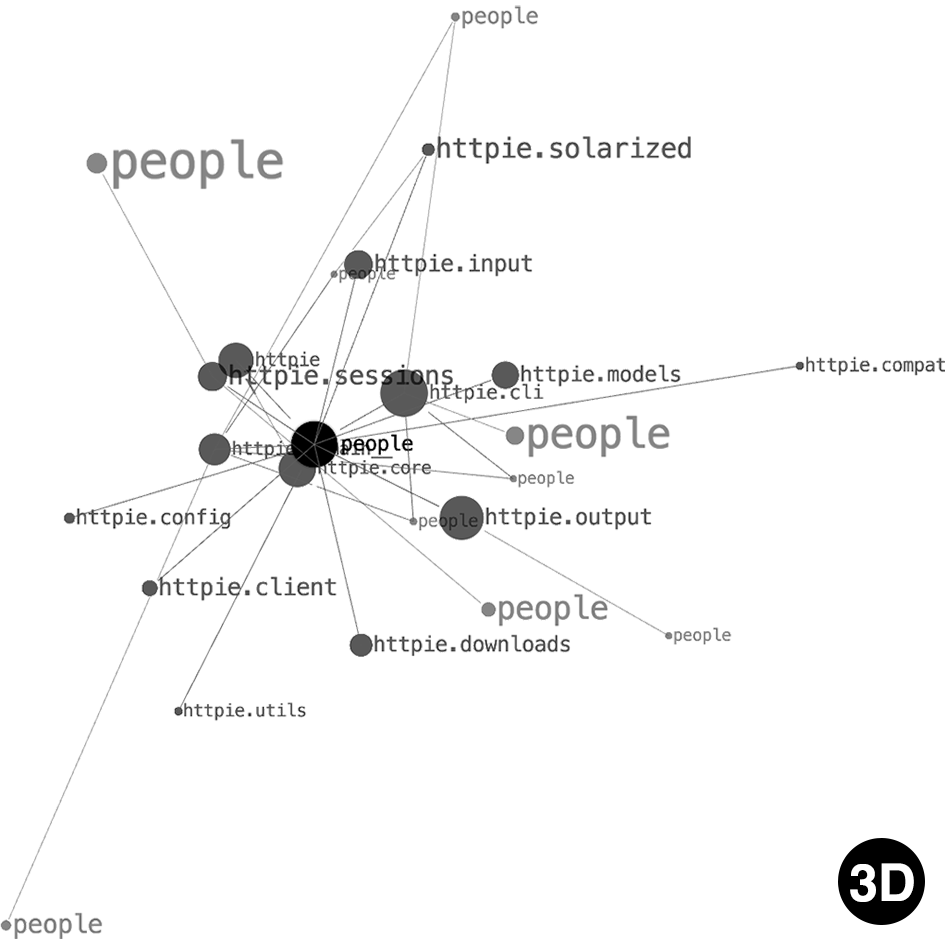
\includegraphics[width=0.48\linewidth]{images/labels1}%
	}%
	\hfill
	\subfloat[Second perspective]{%
		\label{fig:pos2}%
		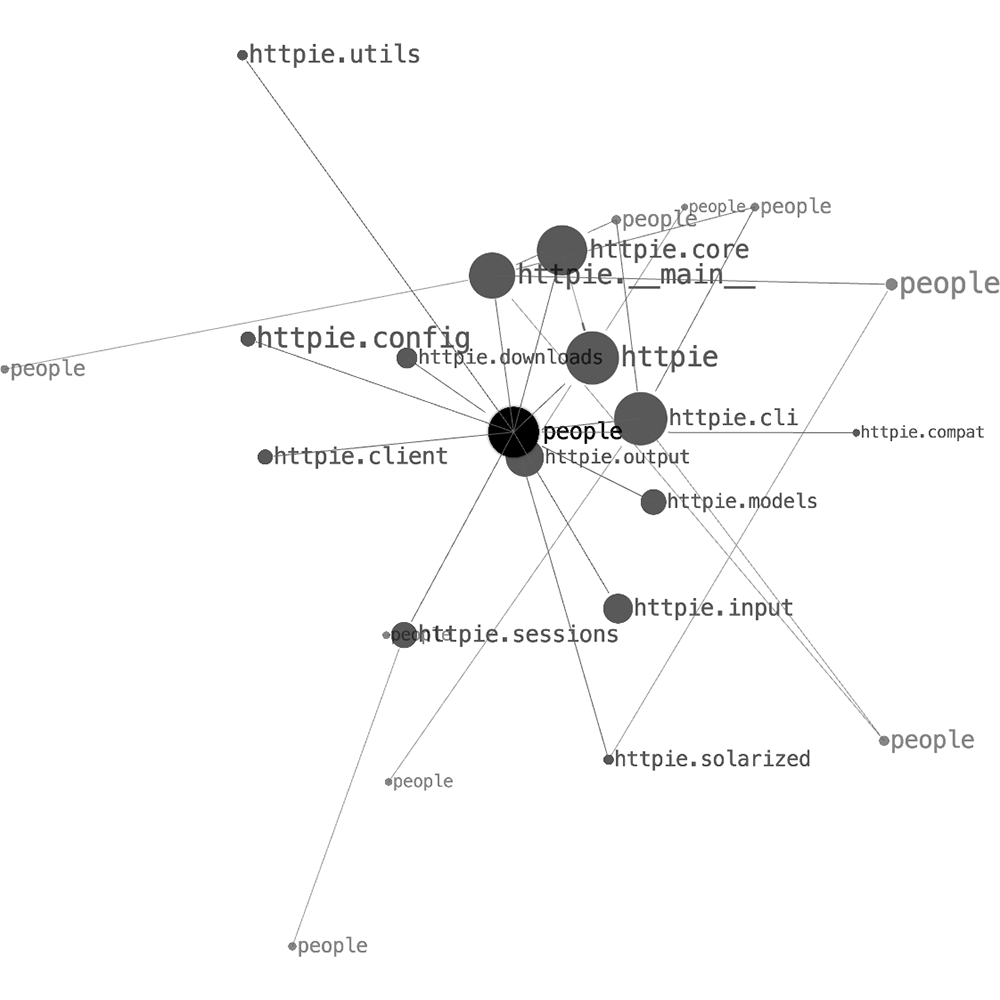
\includegraphics[width=0.48\linewidth]{images/labels2}%
	}%
  \caption[Two different perspectives of the same graph.]{Two different perspective of a graph (only a \gls{3d} rotation was applied, the layout is the same for both images).}%
  \label{fig:labels}
\end{figure}

\p{A hackish solution}
The implemented solution to the problem is interesting and deserves to be explained in depth. As the goal was to obtain the best performance while meeting the requirements previously explained, we tried to offload all possible computations to the \gls{gpu}. For this reason we implemented a custom shader capable of both positioning and drawing the labels without intervention of the \gls{cpu}.

\p{Model}
For the purpose of our implementation, we create a custom geometry containing a \emph{quad} (a face with 4 vertices) for each character of each label in the graph, as shown by the red dots in \vref{fig:label-construction}. Instead of adding them at their correct offset (as shown in the figure), we all add them at the same coordinates as the center of the node (line 20 of \vref{lst:labels-cpu}). Along with the position, we also pass other attributes to the \gls{gpu}, such as the node size (line 28), the opacity, the visibility, and the color (not shown in the code).

\begin{figure}[p]
  \centering
  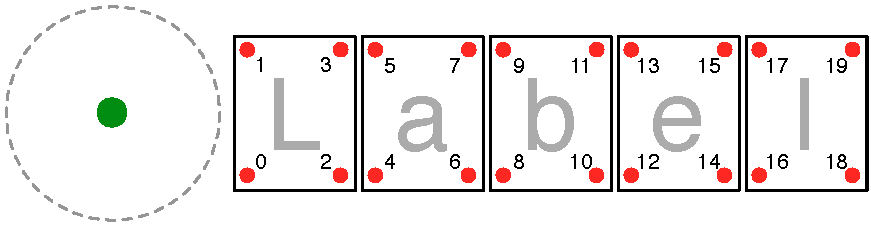
\includegraphics[width=.8\linewidth]{images/label-construction}
  \caption[Construction of the label for a node.]{Schematic construction of a node label. The green dot on the left is the center of the node, the red dots inside the rectangles are the vertices used to construct the faces.}
  \label{fig:label-construction}
\end{figure}

\p{Characters drawing}
Instead of passing a list of characters to display on each face to the \gls{gpu}, we generate a texture by means of the code shown in \ref{lst:labels-texture}. We then populate the texture position vector of each face with the offsets for the right character (lines 12--18 and 29--34 of \ref{lst:labels-cpu}). The resulting texture and the positioning principle are shown in the two subfigures of \vref{fig:label-texture}.

\begin{figure}[p]
  \begin{adjustwidth}{0mm}{-0.1mm}  
    \subfloat[Complete texture]{%
      \label{fig:texture}%
      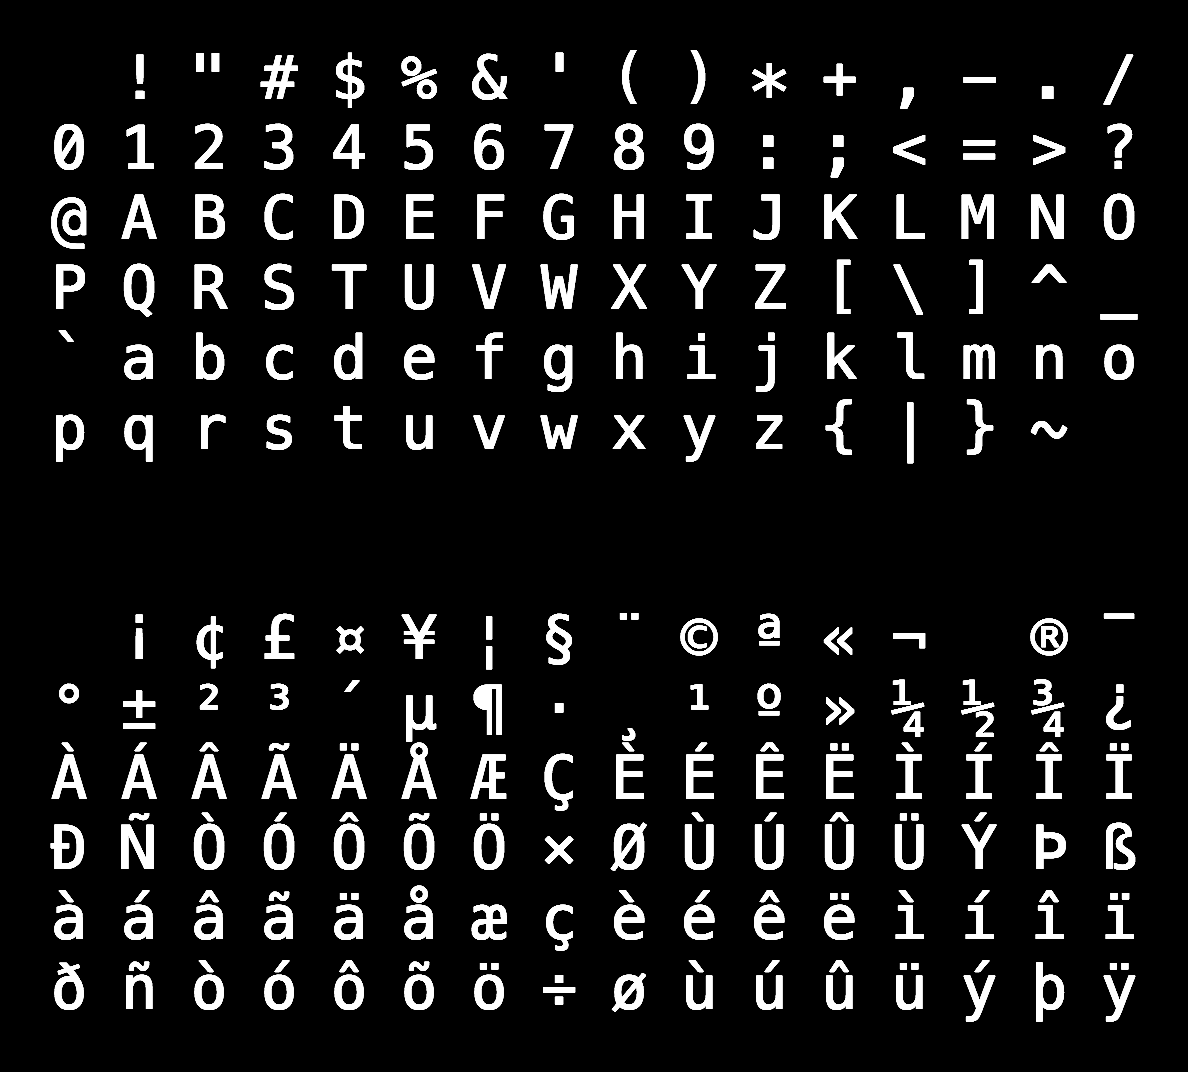
\includegraphics[height=6cm]{images/texture}%
    }%
    \hfill
    \subfloat[Texture positioning]{%
      \label{fig:positioning}%
      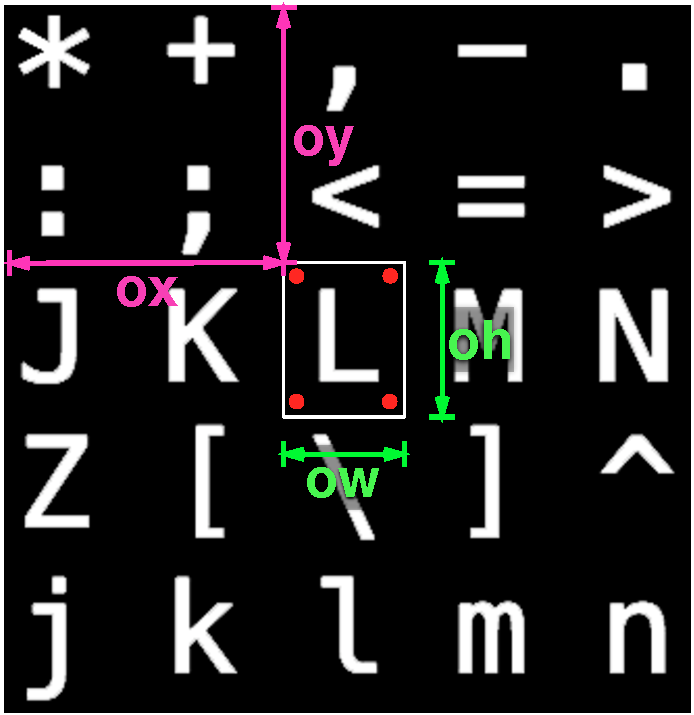
\includegraphics[height=6.04cm]{images/label-texture}%
  	}
  \end{adjustwidth}
  \caption[Generated texture used to draw the text.]{Generated texture and its usage to draw the label characters during the rendering.}%
  \label{fig:label-texture}
\end{figure}

\begin{figure}
\begin{lstlisting}[caption={Initial creation of the labels in-memory representation.},label=lst:labels-cpu,language=javascript]
populate: (geometry) =>
    globalCharIndex = 0

    ow = TEXTURE_CHAR_WIDTH / (FONT_SIZE * LETTERS_PER_SIDE)
    oh = TEXTURE_CHAR_HEIGHT / (FONT_SIZE * LETTERS_PER_SIDE)

    @model.nodes.iter((node, i) =>
        position = node.getAbsolutePosition()
        size = node.getSize()

        for char, j in node.getLabel()
            charCode = char.charCodeAt(0)

            charX = charCode % LETTERS_PER_SIDE
            charY = Math.floor(charCode / LETTERS_PER_SIDE)

            ox = (charX + 0.5) / LETTERS_PER_SIDE - ow / 2.0
            oy = (LETTERS_PER_SIDE - charY - .5) / LETTERS_PER_SIDE - oh / 2.0

            geometry.vertices.push(position, position, position, position)
            geometry.faces.push(new THREE.Face4(
                globalCharIndex * 4,
                globalCharIndex * 4 + 1,
                globalCharIndex * 4 + 2,
                globalCharIndex * 4 + 3
            ))
            @chars.push(j * 4 + 1, j * 4 + 0, j * 4 + 2, j * 4 + 3)
            @sizes.push(size, size, size, size)
            geometry.faceVertexUvs[0].push([
                new THREE.Vector2(ox, oy + oh),
                new THREE.Vector2(ox, oy),
                new THREE.Vector2(ox + ow, oy),
                new THREE.Vector2(ox + ow, oy + oh),
            ])

            globalCharIndex++
    )
\end{lstlisting}
\end{figure}

\begin{figure}
\begin{lstlisting}[caption={Dynamic creation of the texture.},label=lst:labels-texture,language=javascript]
@makeTexture: ->
    c = document.createElement('canvas')
    c.width = c.height = sz = FONT_SIZE * LETTERS_PER_SIDE
    ctx = c.getContext('2d')
    ctx.font = (FONT_SIZE - 10) + 'px menlo'
    ctx.fillStyle = "#ffffff"
    yOffset = -0.25

    for y in [0...LETTERS_PER_SIDE]
        for x in [0...LETTERS_PER_SIDE]
            ch = String.fromCharCode(y * LETTERS_PER_SIDE + x)
            ctx.textAlign = "center"
            ctx.fillText(ch, (x + .5) * FONT_SIZE,  (yOffset + y + 1) * FONT_SIZE)

    return new THREE.Texture(c)
\end{lstlisting}
\end{figure}

\p{Vertex shader}
The code discussed until this point needs to run only once (and every time the labels content changes). The remaining part of the implementation runs completely on the \gls{gpu} in the form of a shader. In the \emph{Model} paragraph above we stated that all vertices are added at the position of the node, regardless of character their face represents. The reason for this is that the correct final position needs to be recalculated each time the user modifies the viewport and this is best done on the \gls{gpu}. The calculation of the final coordinates where a vertex has to be drawn is exactly the task of a \emph{vertex shader}. \Vref{lst:label-vertex} contains the implementation of the custom shader taking care of the correct positioning of the vertices. The presented implementation also takes care of adapting the font size to the node size.

\begin{figure}
\begin{lstlisting}[caption={Vertex shader for the final positioning of the label vertices (GLSL).},label=lst:label-vertex,language=c]
varying vec2 vUv;
varying float fontSize;
attribute float nodeSize;
attribute float char;
uniform float nodeSizeFactor;
uniform float baseSize;
uniform float sizeRatio;
uniform float widthRatio;

attribute float labelOpacity;
varying float opacity;

attribute float labelVisibility;
varying float visible;

void main() {
    // Define font size
    fontSize = nodeSize * nodeSizeFactor + baseSize * sizeRatio / 10.0;
    float charWidth = fontSize * 0.2;
    float charHeight = charWidth * 2.0;
    charWidth /= widthRatio;

    // Offset from the center of the node due to node size
    float offset = nodeSize / 23.0 / widthRatio * sizeRatio;

    // Get the projected position and apply sizing
    vec4 pos = projectionMatrix * modelViewMatrix * vec4(position, 1.0);
    pos.x += offset;
    pos.x += floor((floor(char / 2.0) + 1.0) / 2.0) * charWidth;
    pos.y += (mod(char, 2.0) - 0.5) * charHeight;

    // Assign to varying variables for the fragment shader
    visible = labelVisibility;
    opacity = labelOpacity;
    gl_Position = pos;
    vUv = uv;
}
\end{lstlisting}
\end{figure}

\p{Fragment shader}
Once the final positions of the vertices are defined, the \gls{gpu} invokes the fragment shader to decide how the pixels contained by the face shall be painted. By providing a custom fragment shader and reading the previously set values, we can paint the face with the texture chunk set on the \gls{cpu} side at object construction time. The code of the fragment shader is shown in \vref{lst:label-fragment}.

\begin{figure}
\begin{lstlisting}[caption={Fragment shader to paint each face with the correct character.},label=lst:label-fragment,language=c]
uniform vec3 color;
uniform sampler2D texture;
varying vec2 vUv;
varying float opacity;
varying float fontSize;
varying float visible;
void main() {
    if (visible == 0.0) discard;
    gl_FragColor = vec4(color, 1.0);
    gl_FragColor = gl_FragColor * texture2D(texture, vUv);
    gl_FragColor.a *= opacity;
}
\end{lstlisting}
\end{figure}

\p{High performance}
By adopting the described implementation, we were able to obtain notable performances on all the tested graphs. The rendering of a graph with \numprint{16000} nodes and an average label length of 12 characters ($>800k$ vertices!), maintained a constant frame rate of 30 fps even during viewport rotations and other animations. Most importantly, the \gls{cpu} usage was not affected at all, proving that the computations were correctly offloaded to the \gls{gpu}.

\p{Drawbacks}
The main drawback encountered while using the application with this configuration is the quality of the rendered text. By using a bitmap texture instead of the proper typographic hooks normally available such as vectorial fonts, ligatures, proportional spacing, etc. the quality of the rendering is clearly affected. An additional drawback is the complexity of the implementation and its demand in term of \gls{gpu} resources.

\subsection{Asynchronous layouts}

\p{Introduction}
The previous subsections all discussed problems related to optimizations of the rendering performance. In this subsection we tackle another problem connected with performance issues: graph layout algorithms. During the implementation of the visualization application we worked with synchronous layouts running in the same thread as the \gls{ui} for most of the time. At some point, the graphs we wanted to lay out became too big and the layout algorithms began to freeze the user interface. For this reason, we decided to implement an asynchronous version of a layout algorithm.

\p{Web workers}
In the web-applications world almost all code run in one main thread, until the \emph{web workers \gls{api}} was announced as part of the \gls{html} 5 specification. By using \emph{web workers} it is possible to run code in separate background threads without impacting the responsiveness of the main thread. Web worker threads are completely isolated one from another (they do not share any context) and all interactions have to pass through messages.

\p{Design}
Support for asynchronous layouts is provided by a special \texttt{Layout} subclass called \texttt{Worker\BreakableSlash{}Layout} (or simply \emph{proxy} in the next paragraphs). This subclass exposes the same interface as any other layout algorithm but defers the work to a separate thread behind the scenes. The corresponding class with which the \texttt{WorkerLayout} instance communicates is a subclass of \texttt{LayoutWorker} (or simply \emph{worker}).

\p{Transferable objects}
When the worker is first created, the proxy sends a list of nodes and edges. When the worker is run, it will simply send back a list of positions. As graphs get bigger, continuously copying lists of nodes, edges, and positions back and forth can become expensive. To obviate to this problem, we take advantage of \emph{Transferable Objects} \cite{webworker}. Transferable objects allow to transfer ownership of a certain object from a thread to another.\footnote{Currently only \texttt{ArrayBuffer} objects can be transferred.} The referenced object becomes unavailable in the calling thread, but it is transferred with a zero-copy operation. An example of transferable-objects passing is shown in \vref{lst:send-update} and \vref{lst:update-positions} for the worker and proxy, respectively.

\begin{figure}
\begin{lstlisting}[caption={Method used to send position updates from the worker to the proxy.},label=lst:send-update,language=javascript]
sendUpdate: (force=false) ->
    if not force
        if @lastUpdate?
            if Date.now() - @lastUpdate < @minUpdateInterval
                return

    nodes = @nodes

    posx = makeArray(Float32Array, nodes.length)
    posy = makeArray(Float32Array, nodes.length)
    posz = makeArray(Float32Array, nodes.length)

    @nodes.iter((n, i) ->
        posx[i] = n.position.x
        posy[i] = n.position.y
        posz[i] = n.position.z
    )

    @sendMessage('updatePositions', [
        posx.buffer, posy.buffer, posz.buffer
    ], [
        posx.buffer, posy.buffer, posz.buffer
    ])

    @lastUpdate = Date.now()
\end{lstlisting}
\end{figure}

\begin{figure}
\begin{lstlisting}[caption={Method handling the position update messages on the proxy.},label=lst:update-positions,language=javascript]
remote_updatePositions: (posx, posy, posz) ->
    posx = new Float32Array(posx)
    posy = new Float32Array(posy)
    posz = new Float32Array(posz)

    @nodes.iter((n, i) ->
        p = new THREE.Vector3(posx[i], posy[i], posz[i])
        n.setPosition(p)
    )
    @_fire('step')
\end{lstlisting}
\end{figure}

\p{Updates coalescing}
In order to avoid too much overhead due to the message passing, we limit the rate at which the updated positions are transmitted to the client by coalescing updates based on their timestamp. The implementation is very simple and was already shown in lines 2--5 of \vref{lst:send-update}.

\subsection{Other noteworthy aspects}
\label{sec:visu/implementation/other}

\p{Introduction}
In this subsection we briefly present other minor interesting aspects of the implementation which did not already find their way into the preceding subsections.

\p{Iterators}
The first aspect we discuss was already introduced in precedence during the discussion of both the graph model and the layout algorithms. In order to provide an efficient way to iterate over arbitrary sequences of edges and nodes, we introduced the \emph{Iterator pattern}. We accomplished this by extending the base \texttt{Object} prototype with an additional \texttt{iter} method as shown in \vref{lst:iter}. It is now possible to iterate over objects implementing the \texttt{\_\_iterator\_\_} method by simply calling the \texttt{iter} method with a callback function as shown in \vref{lst:iteration}. For added convenience, we provide basic implementations for the most common iterator types, such as \texttt{ArrayIterator}, \texttt{ArrayPropertyIterator} and \texttt{FlattenIterator}. Reusable iterators can be constructed with the \texttt{IteratorFactory} class. The source code for the \texttt{ArrayIterator} and its dynamic addition to the \texttt{Array} prototype chain is shown in \vref{lst:array-iter}.

\begin{figure}
\begin{lstlisting}[caption={Extension of the base prototype with the \texttt{iter} method.},label=lst:iter,language=javascript]
class StopIteration extends Error

Object.defineProperty(Object.prototype, 'iter', {
    value: (cb) ->
        iterator = this.__iterator__()
        i = 0
        while true
            try
                cb(iterator.next(), i)
                i += 1
            catch e
                if e == StopIteration
                    break
                else
                    throw e
        return
    enumerable: false
})
\end{lstlisting}
\end{figure}

\begin{figure}
\begin{lstlisting}[caption={Simple iteration over an iterable object.},label=lst:iteration,language=javascript]
object.iter((item, index) ->
    console.log(index + ': ' + item)
)
\end{lstlisting}
\end{figure}

\begin{figure}
\begin{lstlisting}[caption={Extension of the \texttt{Array} object with the iterator pattern.},label=lst:array-iter,language=javascript]
class ArrayIterator
    constructor: (@array) -> @index = 0
    next: ->
        if @index >= @array.length
            throw StopIteration
        else
            return @array[@index++]

Object.defineProperty(Array.prototype, '__iterator__', {
    value: -> new ArrayIterator(this)
    enumerable: false
})
\end{lstlisting}
\end{figure}

\p{Pan, rotate, zoom and reset}
The next point we discuss in this subsection is the implementation of the different viewport modification functions: panning, rotation, zooming, and reset. All these functions are implemented as standard linear transformations, the notheworthy aspects is their application to an intermediary object instead of directly to the root scene object. By applying the transformation to a dedicated object (enclosing the graph), we avoid to move the whole scene and can support static elements (such as the position indicator in the lower left corner). Additionally, all the matrix multiplications on every single object are carried out on the \gls{gpu}. \Vref{lst:viewport} contains the source code responsible for these four operations.

\begin{figure}
\begin{lstlisting}[caption={Viewport modification functions.},label=lst:viewport,language=javascript]
reset: ->
    @viewer.getMovingObject().scale = new THREE.Vector3(1, 1, 1)
    @viewer.getRotationObject().rotation = new THREE.Vector3(0, 0, 0)
    @viewer.getMovingObject().position = new THREE.Vector3(0, 0, 0)

pan: (offset) ->
    translation = new THREE.Matrix4()
    translation.makeTranslation(
        offset.x * @panSpeed / 10,
        -offset.y * @panSpeed / 10,
        0
    )
    @viewer.getMovingObject().applyMatrix(translation)

zoom: (pos, direction) ->
    camera = @viewer.camera
    scene = @viewer.getMovingObject()

    d = Math.abs(camera.position.z - scene.position.z)
    offset = -direction * @zoomSpeed * (d / 10 + 1)

    # Too far
    if d - offset >= camera.far
        return

    # Too near
    if d - offset < 1
        return

    ax = pos.x - @viewer.container.find('canvas').width() / 2
    ay = pos.y - @viewer.container.find('canvas').height() / 2

    tx = ax * (offset - 1) * @viewer.ratio
    ty = -ay * (offset - 1) * @viewer.ratio

    translation = new THREE.Matrix4()
    translation.makeTranslation(0, 0, offset)
    scene.applyMatrix(translation)

rotate: (offset) ->
    rotationY = new THREE.Matrix4()
    rotationY.makeRotationY(offset.x * @rotationSpeed / 100)
    rotationX = new THREE.Matrix4()
    rotationX.makeRotationX(offset.y * @rotationSpeed / 100)
    rotationZ = new THREE.Matrix4()
    rotationZ.makeRotationZ(offset.z * @rotationSpeed / 100)

    rotation = new THREE.Matrix4().multiplyMatrices(rotationX, rotationY)
    rotation.multiply(rotationZ)

    @viewer.getRotationObject().applyMatrix(rotation)
\end{lstlisting}
\end{figure}

\p{Node selection}
A further interesting problem is the selection of nodes, or better said, the mapping of the mouse coordinates to the \gls{3d} space. This issue can be solved by applying a Ray-Tracing technique to build a list of possible candidates. We can then sort the candidates by their order along the Z-axis to get the topmost node and mark it as active. An excerpt of the code responsible for the selection is available in \vref{lst:raytracing}.

\begin{figure}
\begin{lstlisting}[caption={Raytracing technique used to detect the active node.},label=lst:raytracing,language=javascript]
ray = new THREE.Raycaster()

projector = new THREE.Projector()
vector = new THREE.Vector3(x, y, 0)

origin = @camera.position
direction = vector.clone().sub(origin).normalize()

ray.threshold = 10
ray.set(origin, direction)

candidates = []
@model.domains.iter((domain, i) =>
    intersect = ray.intersectObjects([@domainObjects[i].nodes])
    for obj in intersect
        n = domain.nodes[obj.vertex]
        if n.isVisible()
            if obj.distance <= n.getSize()
                p = n.getAbsolutePosition().clone()
                p.applyMatrix4(@domainObjects[i].nodes.matrixWorld)
                candidates.push([p.z, n])
)

if candidates.length
    candidates.sort()
    node = candidates[candidates.length - 1][1]
    @selectednode = node
else
    @selectednode = undefined
\end{lstlisting}
\end{figure}

\p{Strategies and layout configuration}
The last point we briefly discuss here is the configuration of the strategies and layout factories, and the creation of a new \texttt{Viewer} instance. The goal is to give a taste of the code which has to be modified if a new layout or strategy has to be added.

\begin{figure}
\begin{lstlisting}[caption={Construction of a viewer instance.},label=lst:viewer,language=javascript]
strategies = [
    new SingleStrategy([
        new RandomLayoutFactory(),
        new FRLayout2DAsyncFactory(),
        /* ... */
    ]),
    new DomainStrategy([
        new FRLayout2DAsyncFactory(),  // Intra-domain layouts
        new FRLayout2DFactory(),
    ], [
        new StackedLayoutFactory(),    // Inter-domain layouts
        new FRLayout3DFactory(),
    ]),
    new ExtrudedStrategy([
        new FRLayout2DFactory(),       // Domain layouts
        /* ... */
    ], [
        new DomainFRLayout2DFactory()  // Nodes layouts
        /* ... */
    ]),
    // ...
]

// Build viewer and load graph
new Viewer($('.graph-viewer'), strategies).load($.urlParam('url'))
\end{lstlisting}
\end{figure}

\section{Results}
\label{sec:visu/results}

\p{Introduction}
The many hours spent in the analysis, design, and implementation of a web-based graph visualization application have paid off. We succeeded in both providing a high performance \gls{3d} graph rendering engine running completely in a web browser, and in researching different ways to layout multi-domain networks. In this final section we discuss the different outcomings concerning the visualization application.

\p{\gls{gui} overview}
Before diving into more specific details about the layout engine and the rendering performances, \vref{fig:appvisu} provides a glance of what the final user interface looks like. The global structure of the \gls{ui} is very simple and consists of a main area containing the viewport where the graph is rendered (on the left) and a sidebar hosting different widgets to tweak the visualization and configure the layout engine (on the right).

\begin{figure}
  \centering
  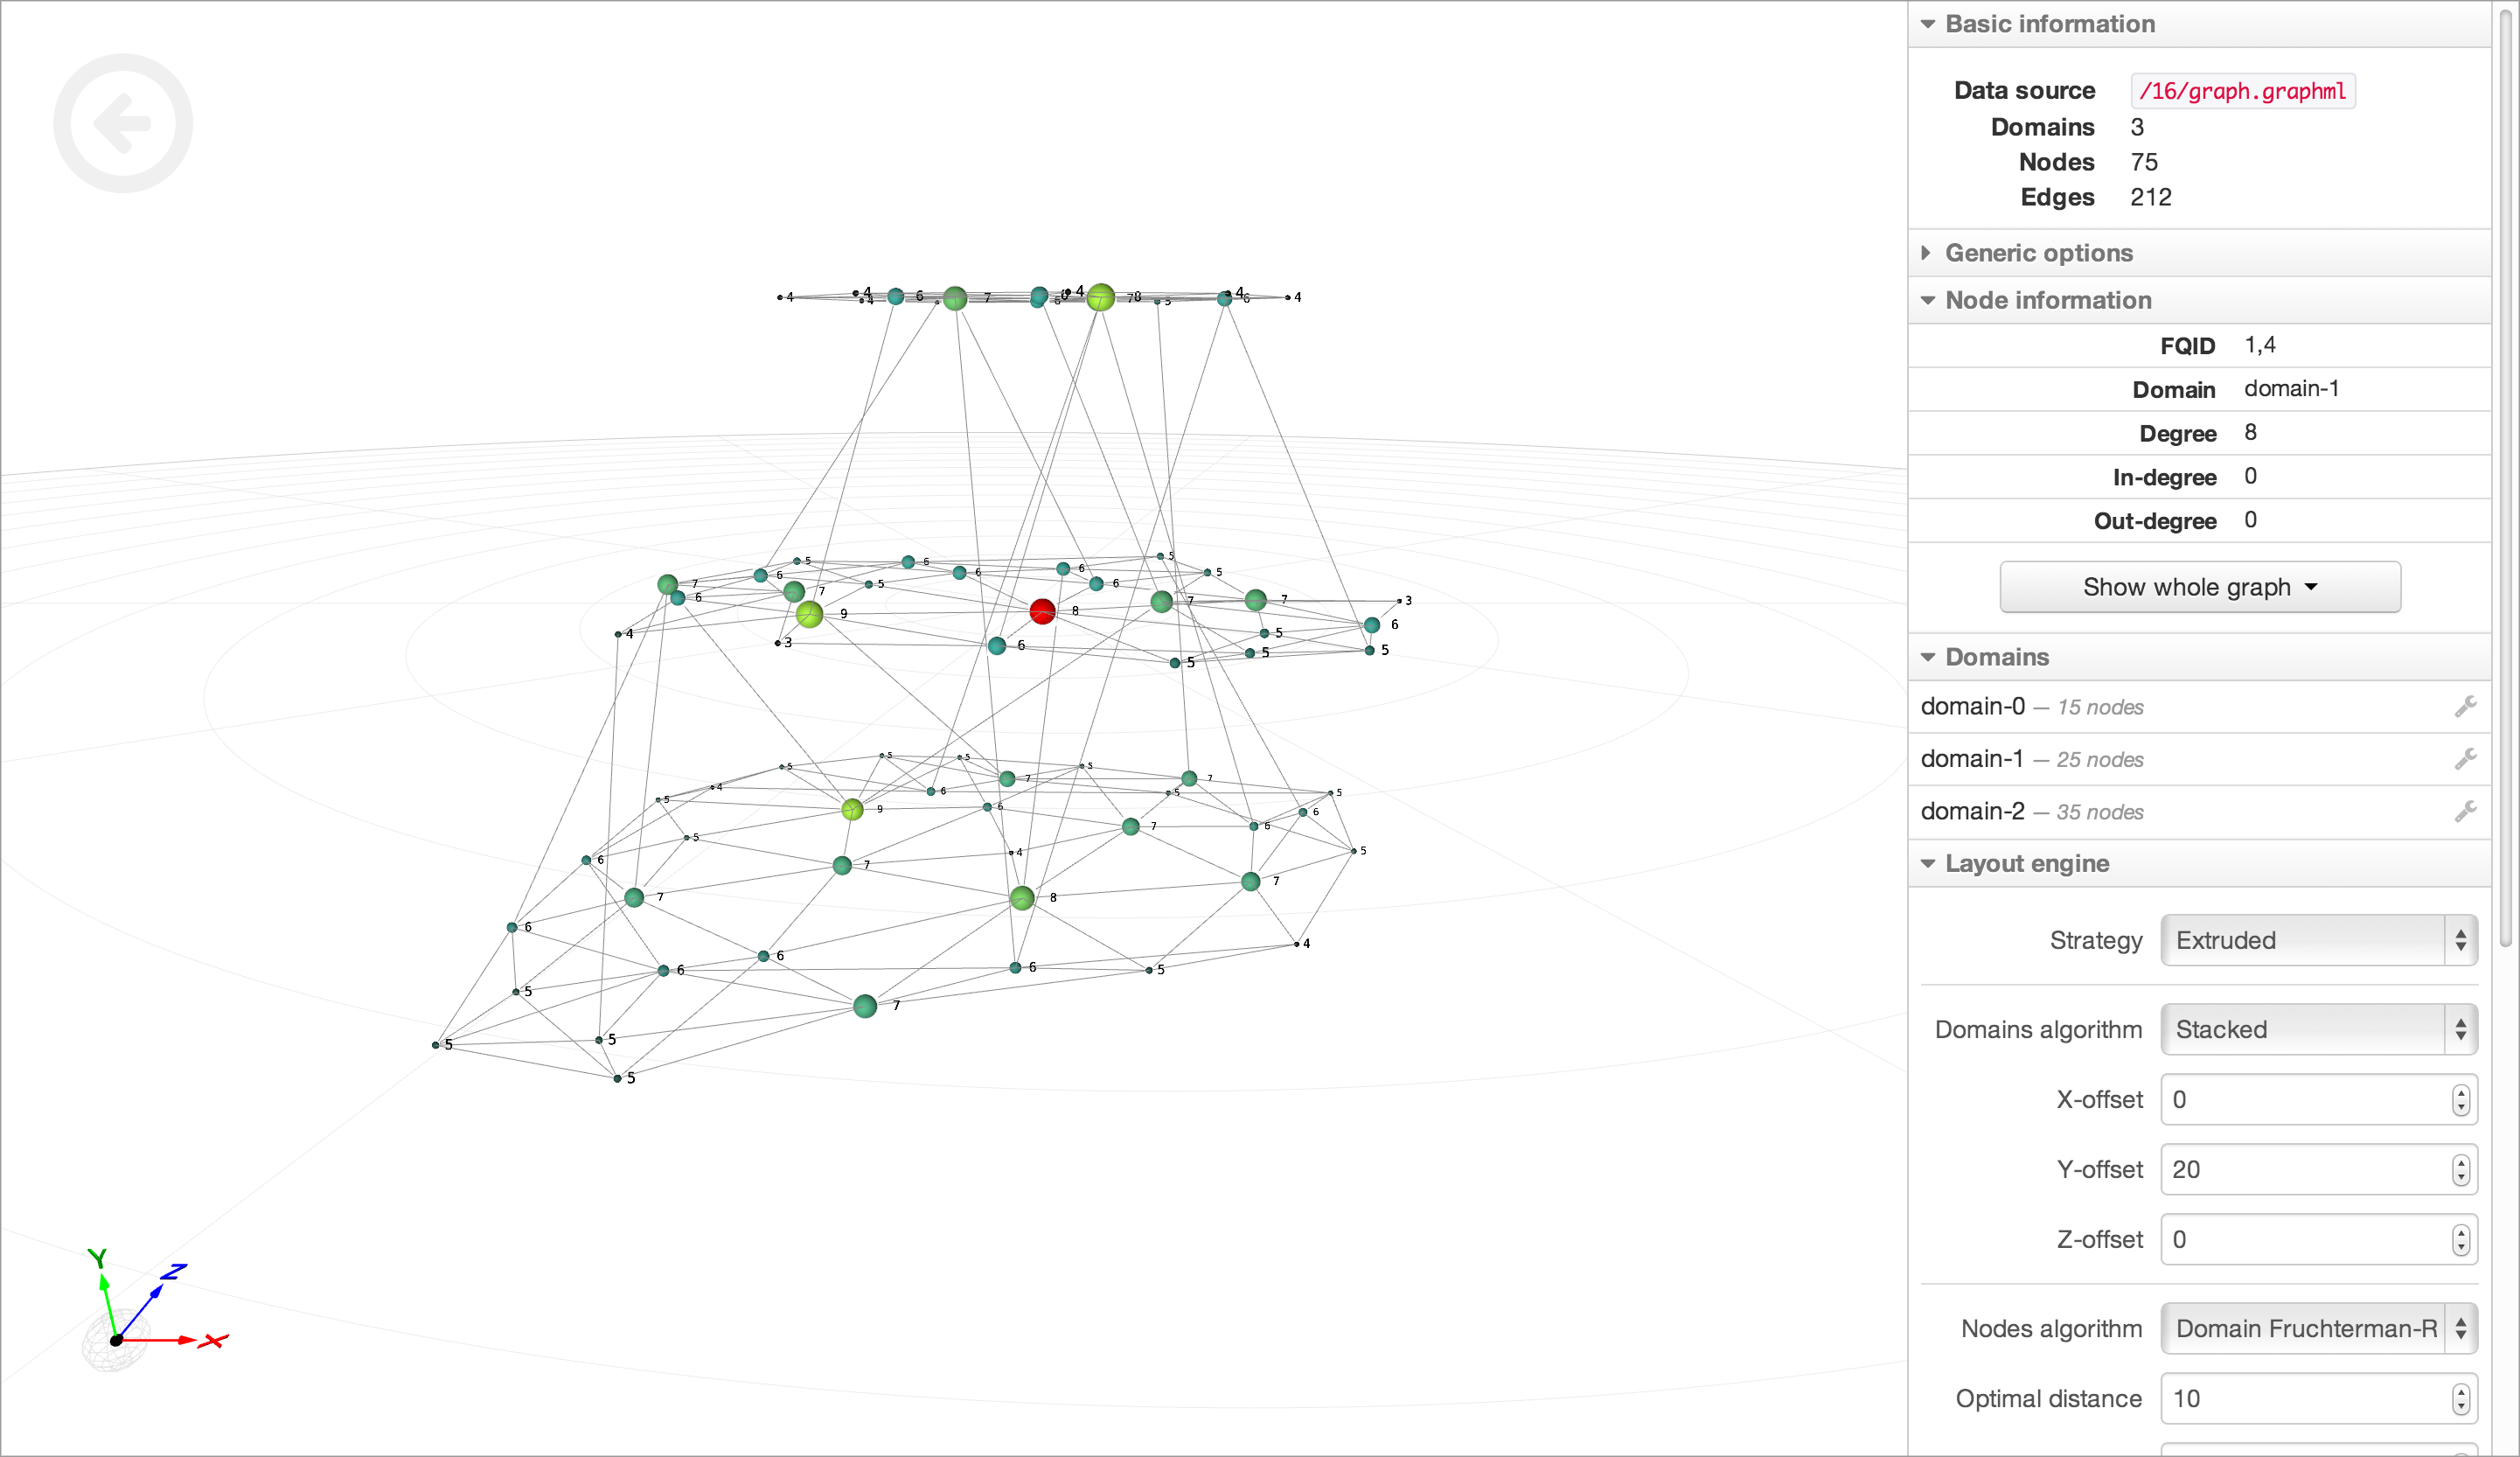
\includegraphics[width=\linewidth]{images/visuapp}
  \caption[Screen shot of the visualization application.]{Screen shot of the final version of the visualization application. The viewport contains a graph with 3 domains, 75 nodes and 212 edges laid out using the extruded strategy and the multi-domain version of the Fruchterman-Reingold layout algorithm.}
  \label{fig:appvisu}
\end{figure}

\p{Structure of the section}
The remaining part of this section focuses primarily on the presentation of the different strategies we researched and then developed as part of the newly introduced model to lay out multi-domain graphs with different properties. Secondarily, we briefly present an empiric performance evaluation of the rendering engine.

\vspace{5mm}
\subsection{Strategies}

\p{Overview}
Throughout the development of the visualization application we continuously tested different multi-domain graphs. During these empirical evaluations of the quality of the visualization we researched different ways to adapt the Strategy/Layout model presented in \vref{sec:visu/analysis} to the various types of encountered graphs. This process resulted in the development of four different strategies which we discuss in the present subsection.

\p{Examples}
%\todo{Uncomment sentence}
To help the presentation of the different strategies we prepared five different graphs to use as examples for the layout algorithms. The results are shown in \vrefrange{fig:ex1}{fig:ex5}, while more details about the graphs used are shown in \vref{tab:graphs}.

\begin{table}
  \vspace{5mm}
  \begin{tabularx}{\textwidth}{c | c | c | c | c | c | c | X }
    \toprule
    \# & $|D|$ & $|V|$ & $|E|$ & $|E_{\mathit{inter}}|$ & $\eta_{i,i}$ & Layouts & Comment\\[.7mm]
    \hline
    1 & 3 & 60 & 200 & 8 & 95\% & \Ref{fig:ex1} & Simple example\\ % Random 2
    2 & 3 & 60 & 200 & 92 & 50\% & \Ref{fig:ex2} & Inconclusive $\eta_{i,i}$ \\ % Random (0.5)
    3 & 3 & 200 & 200 & 35 & 80\% & \Ref{fig:ex3} & Loose structure \\ % Random no structure
    4 & 15 & 600 & 2000 & 171 & 93\% & \Ref{fig:ex4} & Many domains \\ % Many domains
    5 & 3 & 74 & 206 & 20 & 90\% & \Ref{fig:ex5} & Delaunay triangulation \\ % Delaunay

    \bottomrule
  \end{tabularx}

  \caption[Summary of the example graphs.]{Summary of the example graphs. The columns represent: the example \gls{id}, the number of domains, the order of the graph, the size of the graph, the number of inter-domain edges, and the ratio between intra-domain edges and the graph size. The reference to the figure showing the different layouts and a comment are given as well.}
  \label{tab:graphs}
  \vspace{3mm}
\end{table}


\subsubsection{Single}

\p{Principle}
The first implemented strategy is basically a ``pass-through'' middleware to render a multi-domain graph with a single standard layout algorithm. This strategy completely discards the domain information and the final effect is the same as applying the layout algorithm directly to a single-domain graph.

\p{Results}
The final result of the layout of a graph using this strategy completely depends on the used algorithm. For the purpose of multi-domain graphs layout, any algorithm which visually highlights clusters in the dataset can yield good results.

\subsubsection{Multi-level}

\p{Principle}
A natural evolution of the \emph{single} strategy is the \emph{multi-level} approach. This strategy lays out each domain as a single standalone graph, by using an independent and possibly different layout algorithm for each domain. An additional layout algorithm handles the disposition of the domains themselves by considering each domain as a single node.

\p{Advantages and disadvantages}
The obvious advantage of this strategy is the possibility to use different layout algorithms for different domains. As different domains normally model different types of data, it makes sense to choose an adapted layout algorithm for each of them. This is not possible with the single strategy neither it is with the two additional strategies presented below. The equally obvious disadvantage is that this strategy completely ignores the inter-domain edges and can easily lead to messy results for graphs with a low ratio of intra-domain edges.

\p{Examples}
The best results with this strategy were achieved for graphs with many domains, where we can take advantage of a careful dispositions of the domains during the first pass. An example of such a graph is shown in \vref{fig:ex4-multilevel}.

\p{Possible improvement}
A possible improvement is to consider the ``shape'' of each rendered domain and rotate it in order to optimize the inter-domain edges clarity. Note that this addition does not change the position of the domains nor the positions of the nodes relative to the containing domain.

\subsubsection{Extruded}

\p{Principle}
The extruded strategy works as a combination of the single and multi-level strategies. This strategy exploits one layout algorithm to define the position of each domain. At the same time, a second (possibly different) layout algorithm calculates the position of the nodes by considering all part of the same graph. When both layout algorithms return their results, each node is placed at vectorial sum of the position returned by the latter algorithm, and the position of the enclosing domain as returned by the former.

\p{Advantages and disadvantages}
The particularity of this strategy is to yield good layouts for relatively simple multi-domain graphs by choosing specific combinations of algorithms. In our tests, we obtained the best results by combining a stacked layout for the domain positions with a Fruchterman-Reingold layout for the nodes. An example of a layout produced with this combination is shown in \vref{fig:ex1-extruded}.

\p{Specific layout algorithms}
The layout referenced in the previous paragraph, while showing a good repartition of the domains, does not make a good use of the available volume. In fact, nodes belonging to different domains still repulse themselves. In order to avoid this issue, we developed a modified Fruchterman-Reingold layout algorithm called \emph{Domain Fruchterman-Reingold}. Instead of ignoring forces between nodes belonging to different domains altogether (which would yield the same behavior as the multi-level strategy), the layout algorithm ignores only the repelling components, while accounting for the attractive forces of the connected nodes. This algorithm is a natural fit for the extruded strategy, as partially shown in \vref{fig:ex1-extruded-inter} and \vref{fig:ex3-extruded} (to be compared with their multi-level analogous in \vref{fig:ex1-multilevel} and \vref{fig:ex3-multilevel}, respectively).

\p{Edge-clarity tradeoff}
A natural addition to the custom \emph{Domain Fruchterman-Reingold} layout algorithm is a variable weight for inter-domain edges. In fact, by increasing the weight of those edges, we can force the layout algorithm to place two connected nodes belonging to two different domains closer together. When we account for the displacement introduced by the strategy, this yields very clear inter-domain edges, as shown in \vref{fig:ex1-extruded-inter}. The same principle applies when decreasing the weight of those edges. The lower the weights, the less importance the layout engine gives to them, leading to a natural optimization of the intra-domain edges, as shown in \vref{fig:ex1-extruded-intra}. The modifications to the original layout implementation are very simple, as highlighted in \vref{lst:domain-fr}.

\p{Applicability}
An additional interesting note about the edge-clarity tradeoff is that it is a generic technique which can be applied to almost any force-directed layout algorithm and is not limited to the specifics of the Fruchterman-Reingold implementation.

\p{Results}
The inter-domain edge weight can be dynamically adjusted by the user. By exposing this configuration setting as a range slider and calculating the correct weight based on the optimal distance as shown in the lines 2--5 in the preceding listing, the complexity is abstracted away and makes room for interactive experimentation. \Vref{fig:ex5} contains three examples of the same graph laid out with different tradeoff values. The choice of a Delaunay triangulation as graph for each domains makes the tradeoff very visible: intra-domain clarity in the first subfigure inter-domain in the last one.

\subsubsection{Clustered}

\p{Principle}
The last strategy we discuss is the \emph{clustered} strategy. This strategy works as the single strategy in that it wraps a single layout algorithm of choice. Instead of passing through the whole graph to the algorithm, this strategy adds a virtual node for each domain and an edge between each node and its containing domain. This strategy is very good at rendering graphs with a loose structure ($|E| \approx |V|$), but requires the use of an algorithm which naturally highlights clusters.

\p{Example}
An example of the layout of such a graph (graph 3 in \ref{tab:graphs}) is shown in \vref{fig:ex3-clustered}. As apparent from the other subfigures, the creation of virtual clusters helps in visually isolating the domains present in the data set.

\subsection{Graph rendering performance}

\p{Introduction}
The goal of this last subsection is to provide an overview of the performances of the rendering engine for graphs of different order and size. The numbers presented in this subsection are not intended as a precise and exhaustive benchmark of the application, but rather as a tool to get an overview of the size of the graphs supported by it.

\p{System}
The following measurements were done on a MacBook Pro Retina with a 2.7GHz Intel Core i7, 16 GB of \gls{ram}, and an NVIDIA GeForce GT 650M 1024 MB graphic card. The browser used for the tests is Google Chrome version 27.0.1453.116 running under OS X 10.8.4 (12E55). The browser window was opened on an external display (\texttt{devicePixelRatio} $= 1$) and the viewport measured $1650\times1330$ pixels.

\p{Results}
The resulting frame rates obtained during the animation of the chosen graphs are shown in \vref{tab:bench}. The estimate of the number of geometric vertices (the vertices used by the \gls{gpu} to construct the \gls{3d} objects) are shown in the last column. These values can be calculated by applying the following formula
\[
  V_{3D} = (1 + 4 L_{\mathit{LABEL}_\mathit{AVG}}) |V| + 2 |E|
\]
(where $L_{\mathit{LABEL}_\mathit{AVG}}$ is the average label length). A plot of the results is shown in \vref{plt:bench}. As is evident, graphs in the order of $10^4$ nodes and $10^4$ edges are very well supported. Nothing prevents to visualize bigger graphs, in fact the frame rate indicates how many time per second a graph can be redrawn, and lower frame rates only imply non-smooth animations. We would probably hit the memory limit of the browser before other limits due to the number of vertices, but more specific tests would have to be run in order to prove this statement.\footnote{On a related note, Chrome's built-in profiler makes the tab crash when trying to perform a heap snapshot.}

\begin{figure}
\vspace{10mm}
\begin{lstlisting}[caption={Implementation of the \gls{2d} Domain Fruchterman-Reingold layout algorithm.},label=lst:domain-fr,language=javascript]
class DomainFruchtermanReingoldLayout2D extends FruchtermanReingoldLayout2D
    ¶\HighlightFrom¶setInterDomainEdgeWeight: (w) ->¶\HighlightTo¶
    ¶\HighlightFrom¶    if w > 0¶\HighlightTo¶
    ¶\HighlightFrom¶        w *= @k * 2¶\HighlightTo¶
    ¶\HighlightFrom¶    @interWeight = w + 1¶\HighlightTo¶

    _calculateRepulsion: ->
        f_r = (d) => -@k * @k / d

        @nodes.iter((v) =>
            if @onlyVisible and not v.isVisible()
                return
            v._force = new THREE.Vector3(0, 0, 0)
            @nodes.iter((u) =>
                if u == v
                    return
                ¶\HighlightFrom¶if u.domain.id != v.domain.id¶\HighlightTo¶
                ¶\HighlightFrom¶    return  // Ignore inter-domain repulsive forces¶\HighlightTo¶
                d = v.getPosition().clone().sub(u.getPosition())
                f = f_r(d.length())
                v._force.sub(d.normalize().multiplyScalar(f))
            )
            @count++
        )

    _calculateAttraction: ->
        f_a = (d) => d * d / @k

        @edges.iter((e) =>
            [u, v] = [e.src, e.dst]
            d = v.getPosition().clone().sub(u.getPosition())
            l = d.length()
            ¶\HighlightFrom¶if e.src.domain.id != e.dst.domain.id¶\HighlightTo¶
            ¶\HighlightFrom¶    l *= @interWeight  // Adapt weight of inter-domain edges¶\HighlightTo¶
            f = f_a(l) * 2
            f = d.normalize().multiplyScalar(f)
            v._force.sub(f)
            u._force.add(f)
        )
\end{lstlisting}
\vspace{10mm}
\end{figure}

\begin{table}[p]
  \begin{tabularx}{7cm}{c | r | r | c | r }
    \toprule
    $|D|$ & $|V|$ & $|E|$ & $V_{3D}$ & FPS\\[.7mm]
    \hline

      5 &   \numprint{100} &    \numprint{500} & \numprint{4300}    & 60 \\
      5 &   \numprint{500} &   \numprint{2000} & \numprint{20500}   & 60 \\
      5 &  \numprint{1000} &   \numprint{4000} & \numprint{41000}   & 60 \\
     10 &  \numprint{3000} &  \numprint{10000} & \numprint{119000}  & 60 \\
     20 &  \numprint{8000} &  \numprint{20000} & \numprint{304000}  & 55 \\
     30 & \numprint{12000} &  \numprint{25000} & \numprint{446000}  & 54 \\
     40 & \numprint{16000} &  \numprint{30000} & \numprint{588000}  & 50 \\
     40 & \numprint{20000} &  \numprint{40000} & \numprint{740000}  & 36 \\
     40 & \numprint{25000} &  \numprint{80000} & \numprint{985000}  & 26 \\
     50 & \numprint{35000} & \numprint{100000} & \numprint{1355000} & 20 \\
    100 & \numprint{50000} & \numprint{200000} & \numprint{2050000} & 13 \\

    \bottomrule
  \end{tabularx}

  \caption[Frame rate for graphs of different size and order.]{Frame rate for graphs of different size and order.}
  \label{tab:bench}
\end{table}

\begin{figure}[p]
  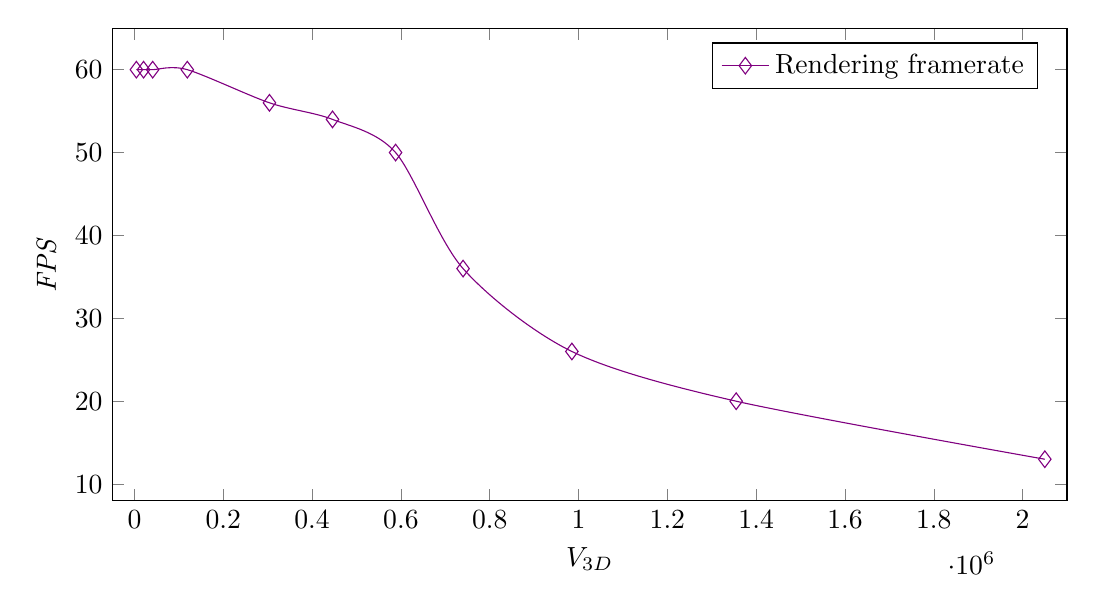
\begin{tikzpicture}
    \pgfplotsset{
      scale only axis,
      set layers,
      width=\linewidth,
      height=6cm,
      legend style={
        legend pos=north east,
      },
      xmin=-50000, xmax=2100000,
    }
    \begin{axis}[
      xlabel=$V_{3D}$,
      ylabel={$\mathit{FPS}$},
      ymin=8, ymax=65,
    ]
      \addlegendentry{Rendering framerate}
      \addplot[smooth,color=violet,mark=diamond,mark size=3] coordinates {
          (4300,60)
          (20500,60)
          (41000,60)
          (119000,60)
          (304000,56)
          (446000,54)
          (588000,50)
          (740000,36)
          (985000,26)
          (1355000,20)
          (2050000,13)
      };
      \label{pgfplot:bench}
    \end{axis}
    \alignOnFrame{0cm}{.9cm}
  \end{tikzpicture}
  \caption[Frame rate for graphs of different size and order.]{Graphical representation of the frame rates presented in \vref{tab:bench} for graphs of different size and order.}
  \label{plt:bench}
\end{figure}

\afterpage{%
    \cleartoodd
\begin{figure}[p]
  \begin{adjustwidth}{0cm}{0cm}
    \vspace{-1cm}
    \setlength{\w}{0.48\linewidth}
    \setlength{\h}{0.28\textheight}
    \subfloat[Single strategy with \gls{2d} Fruchterman-Reingold layout]{%
      \label{fig:ex1-single}%
      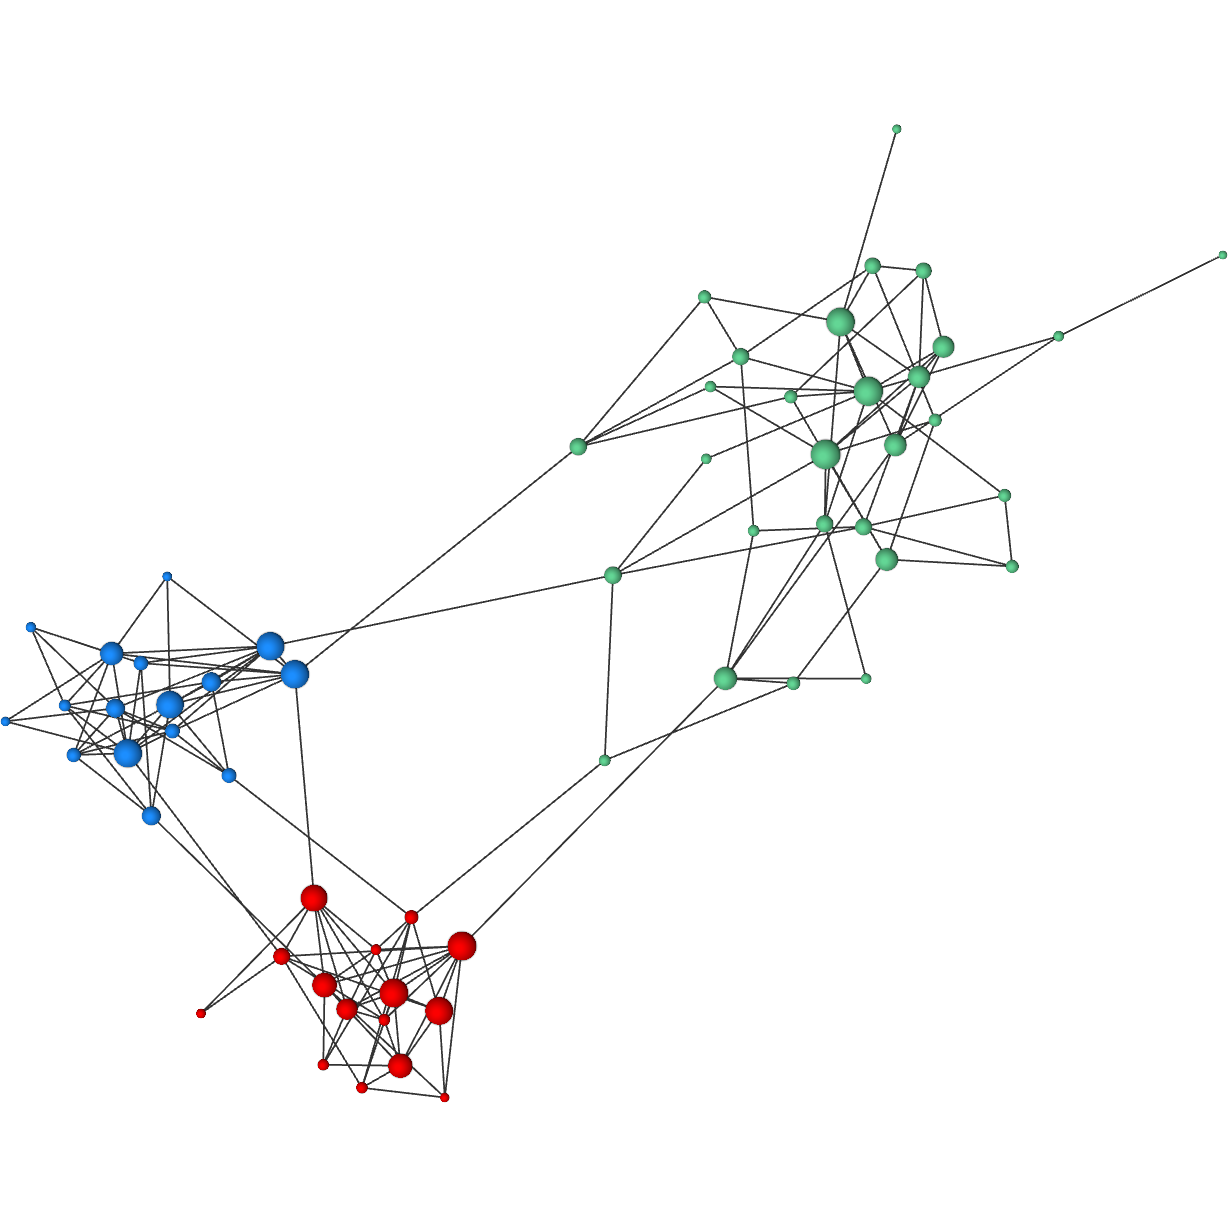
\includegraphics[width=\w,height=\h,keepaspectratio]{images/ex1/single}%
    }%
    \hfill
    \subfloat[Multilevel strategy with stacked layout for the domains and \gls{2d} Fruchterman-Reingold layout for each layer]{%
      \label{fig:ex1-multilevel}%
      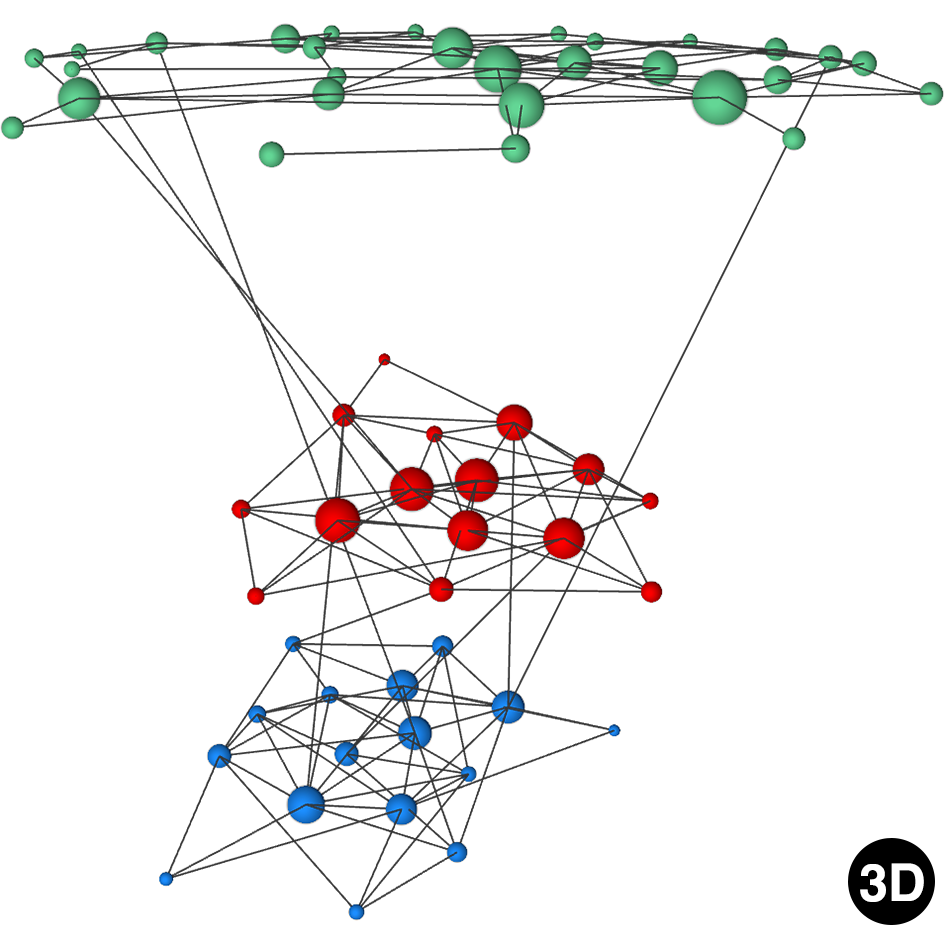
\includegraphics[width=\w,height=\h,keepaspectratio]{images/ex1/multilevel}%
    }\\
    \subfloat[Extruded strategy with Domain \gls{2d} Fruchterman-Reingold layout and enhanced intra-layer clarity]{%
      \label{fig:ex1-extruded-intra}%
      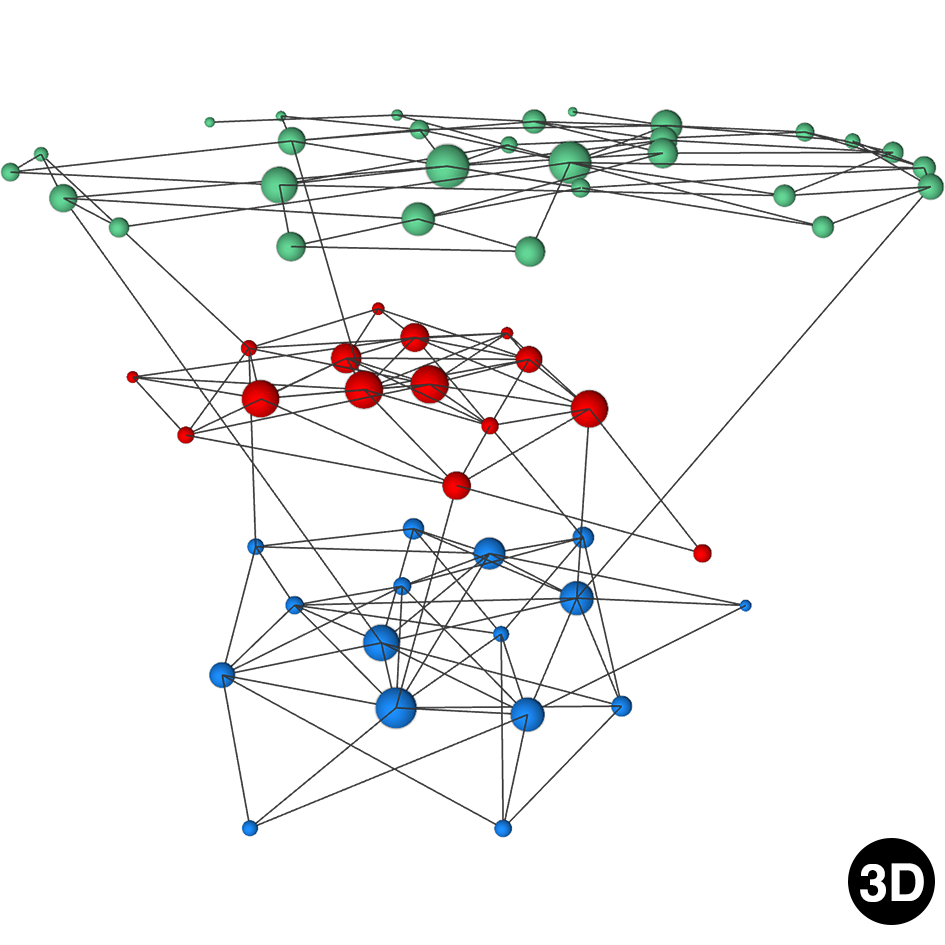
\includegraphics[width=\w,height=\h,keepaspectratio]{images/ex1/extruded-domain-intra}%
    }
    \hfill
    \subfloat[Extruded strategy with Domain \gls{2d} Fruchterman-Reingold layout and enhanced inter-layer clarity]{%
      \label{fig:ex1-extruded-inter}%
      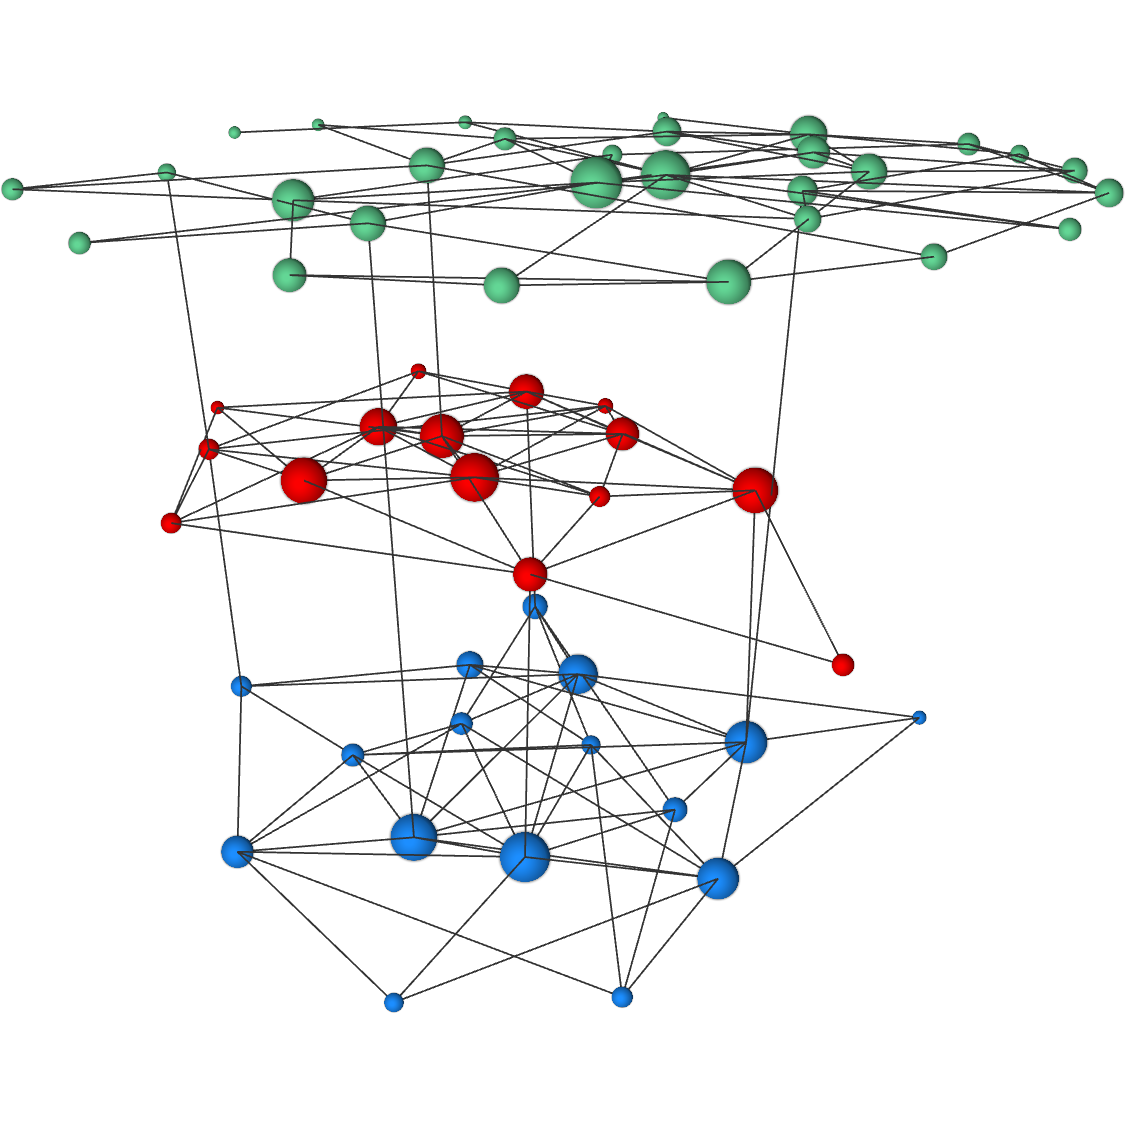
\includegraphics[width=\w,height=\h,keepaspectratio]{images/ex1/extruded-domain-inter}%
    }\\
    \subfloat[Extruded strategy with \gls{2d} Fruchterman-Reingold layout]{%
      \label{fig:ex1-extruded}%
      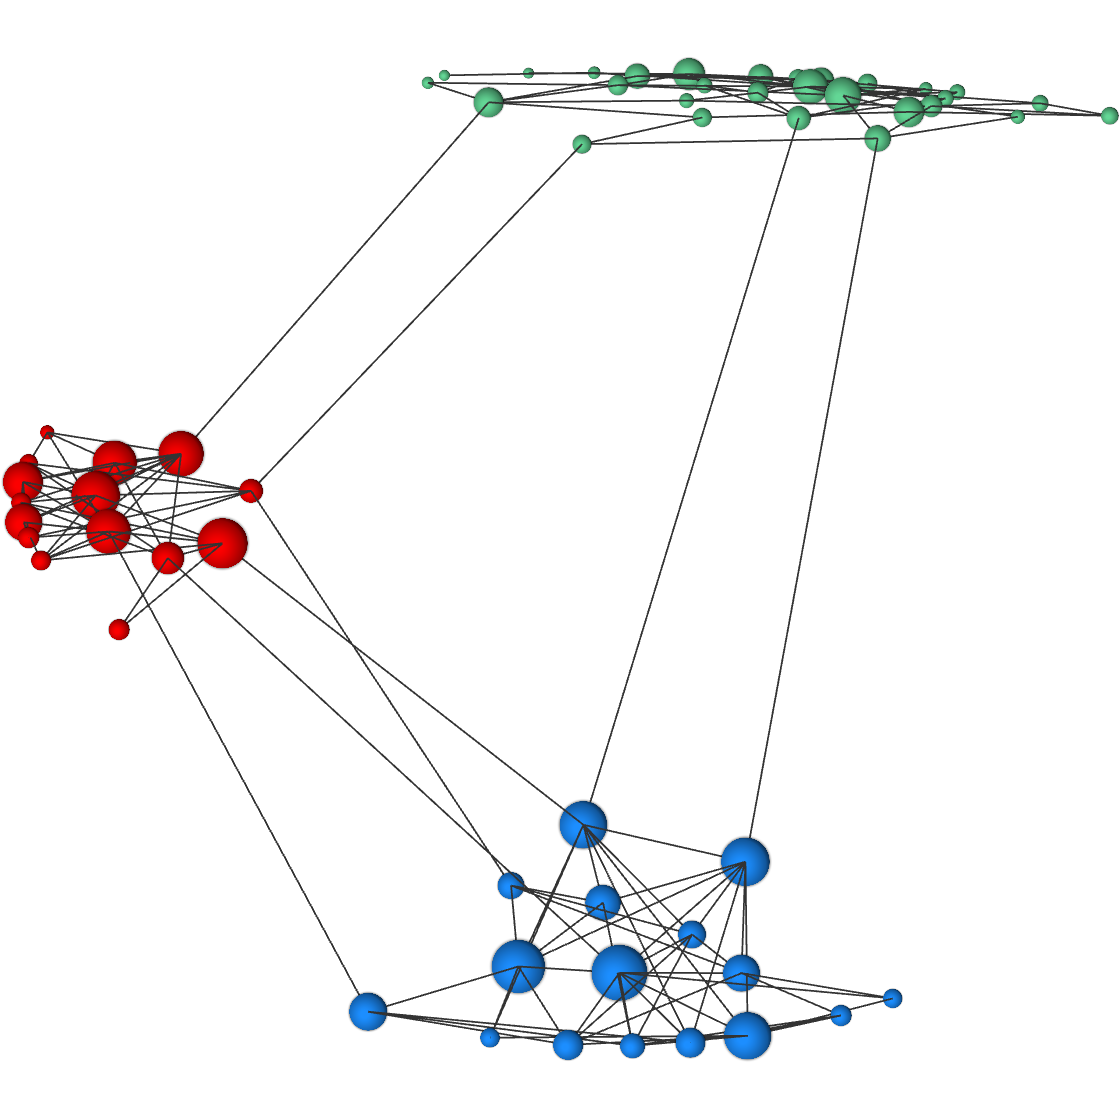
\includegraphics[width=\w,height=\h,keepaspectratio]{images/ex1/extruded}%
    }\\
  \end{adjustwidth}
  \caption[Different layouts for a graph with 3 domains, 60 nodes and 200 edges with a inter-/intra-domain edge ratio of 95\%.]{Different layouts obtained by applying different strategy and layout combinations to a graph with 3 domains, 60 nodes and 200 edges with an inter-/intra-domain edge ratio of 0.9.}%
  \label{fig:ex1}
\end{figure}
  \cleartoodd
}

\afterpage{%
    \cleartoodd
\begin{figure}[p]
  \begin{adjustwidth}{0cm}{-1cm}
    \setlength{\w}{0.48\linewidth}
    \setlength{\h}{0.35\textheight}
    \subfloat[Single strategy with \gls{2d} Fruchterman-Reingold layout]{%
      \label{fig:ex2-single}%
      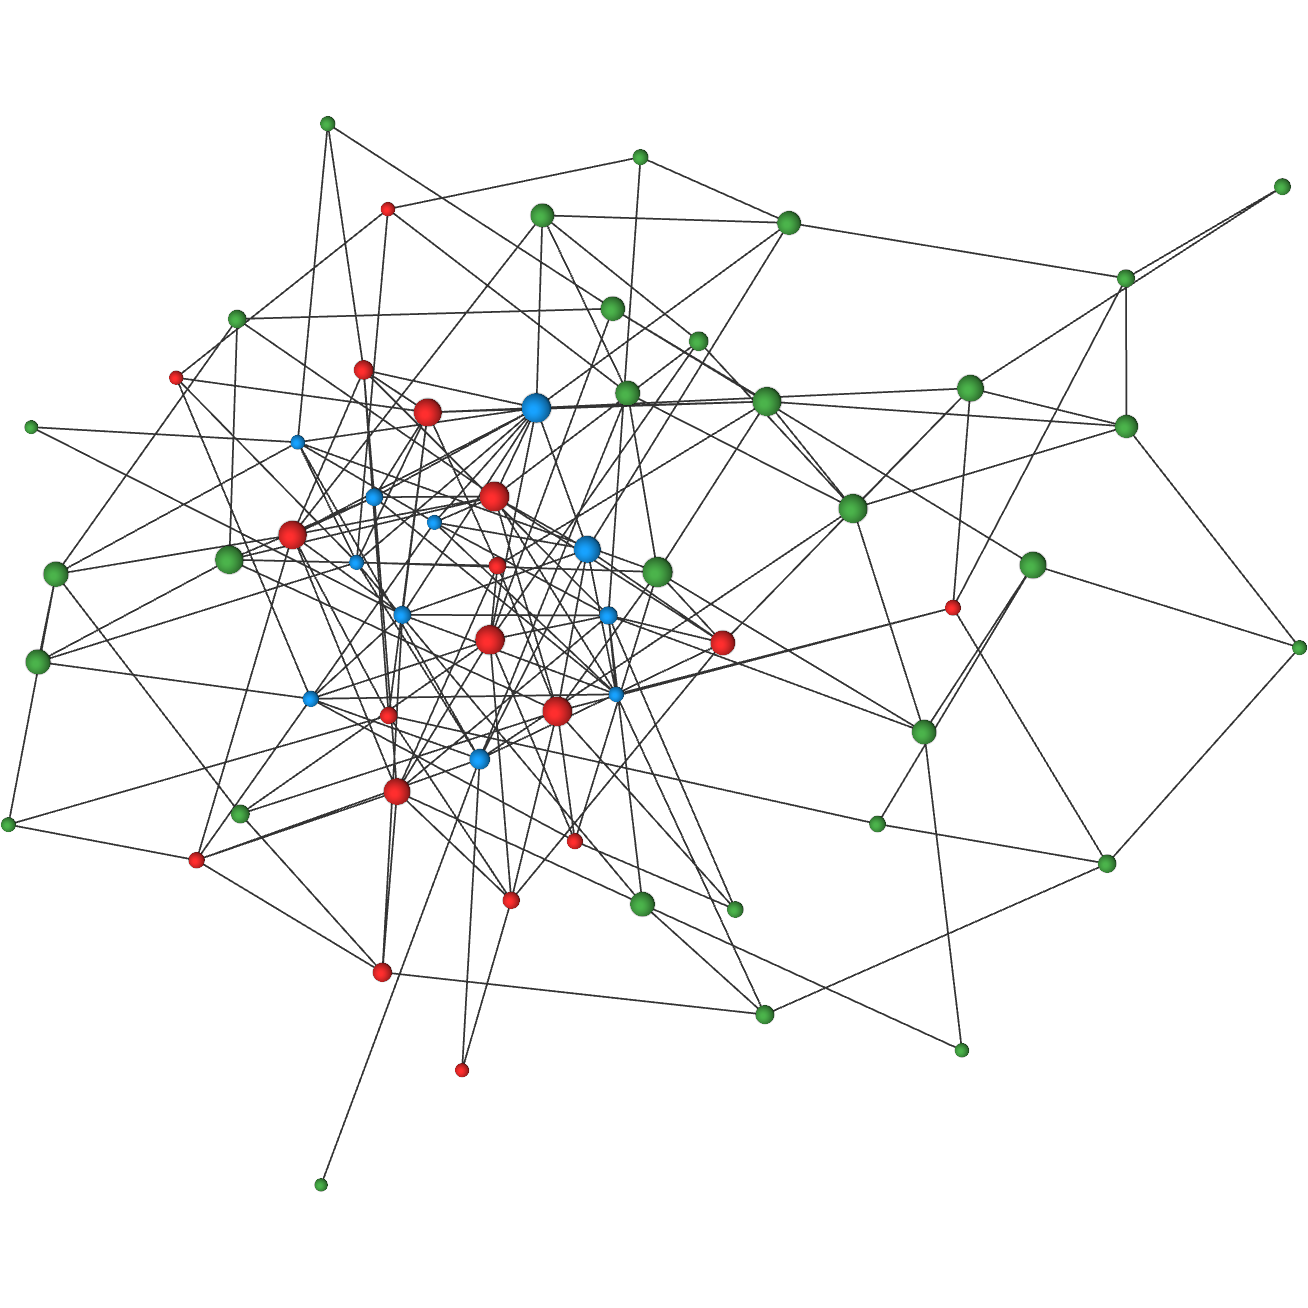
\includegraphics[width=\w,height=\h,keepaspectratio]{images/ex2/single}%
    }%
    \hfill
    \subfloat[Clustered strategy with \gls{2d} Fruchterman-Reingold layout]{%
      \label{fig:ex2-clustered}%
      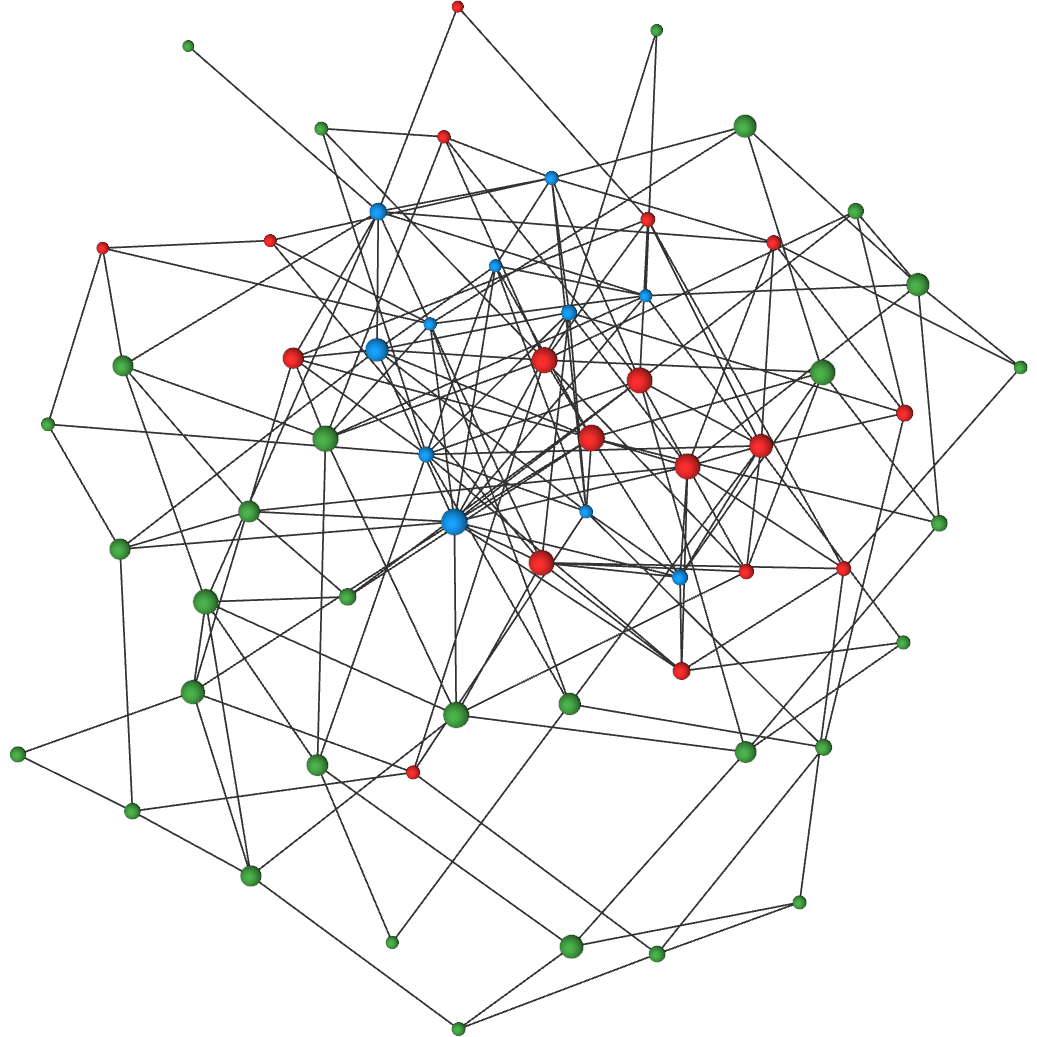
\includegraphics[width=\w,height=\h,keepaspectratio]{images/ex2/clustered}%
    }\\[5mm]
    \subfloat[Multilevel strategy with stacked layout for the domain and \gls{2d} Fruchterman-Reingold layout for each layer]{%
      \label{fig:ex2-multilevel}%
      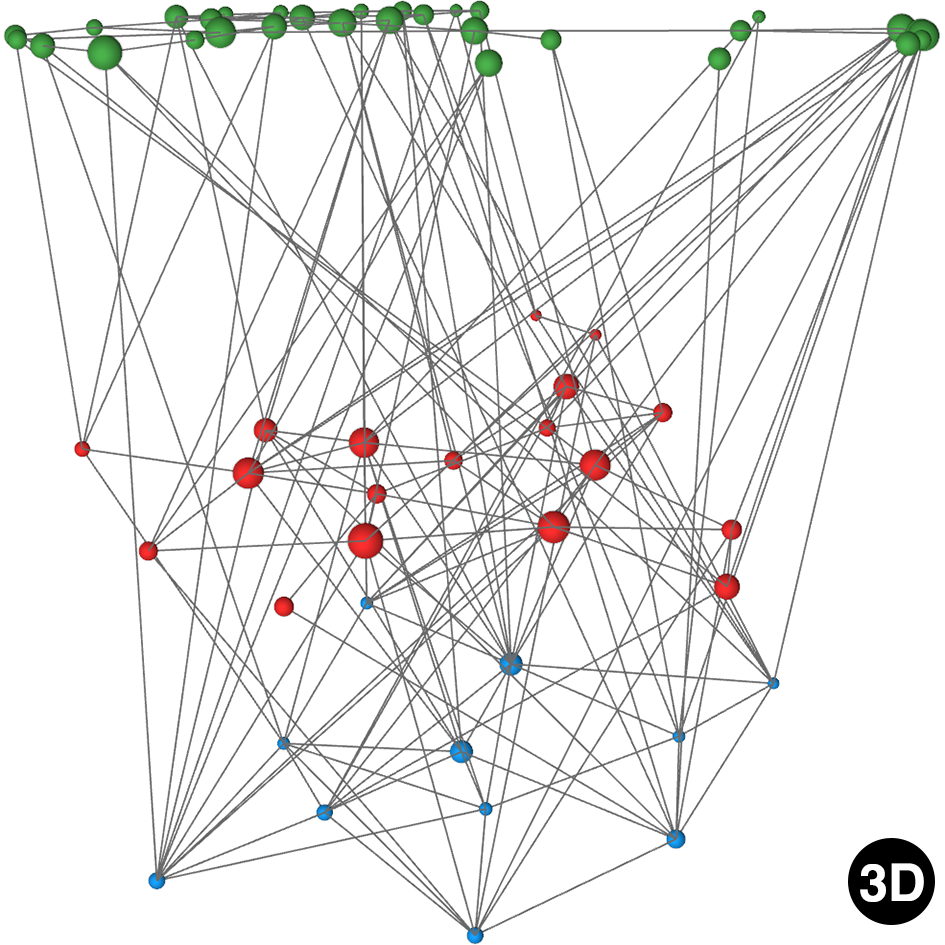
\includegraphics[width=\w,height=\h,keepaspectratio]{images/ex2/multilevel}%
    }\hfill
    \subfloat[Extruded strategy with Domain \gls{2d} Fruchterman-Reingold layout]{%
      \label{fig:ex2-extruded}%
      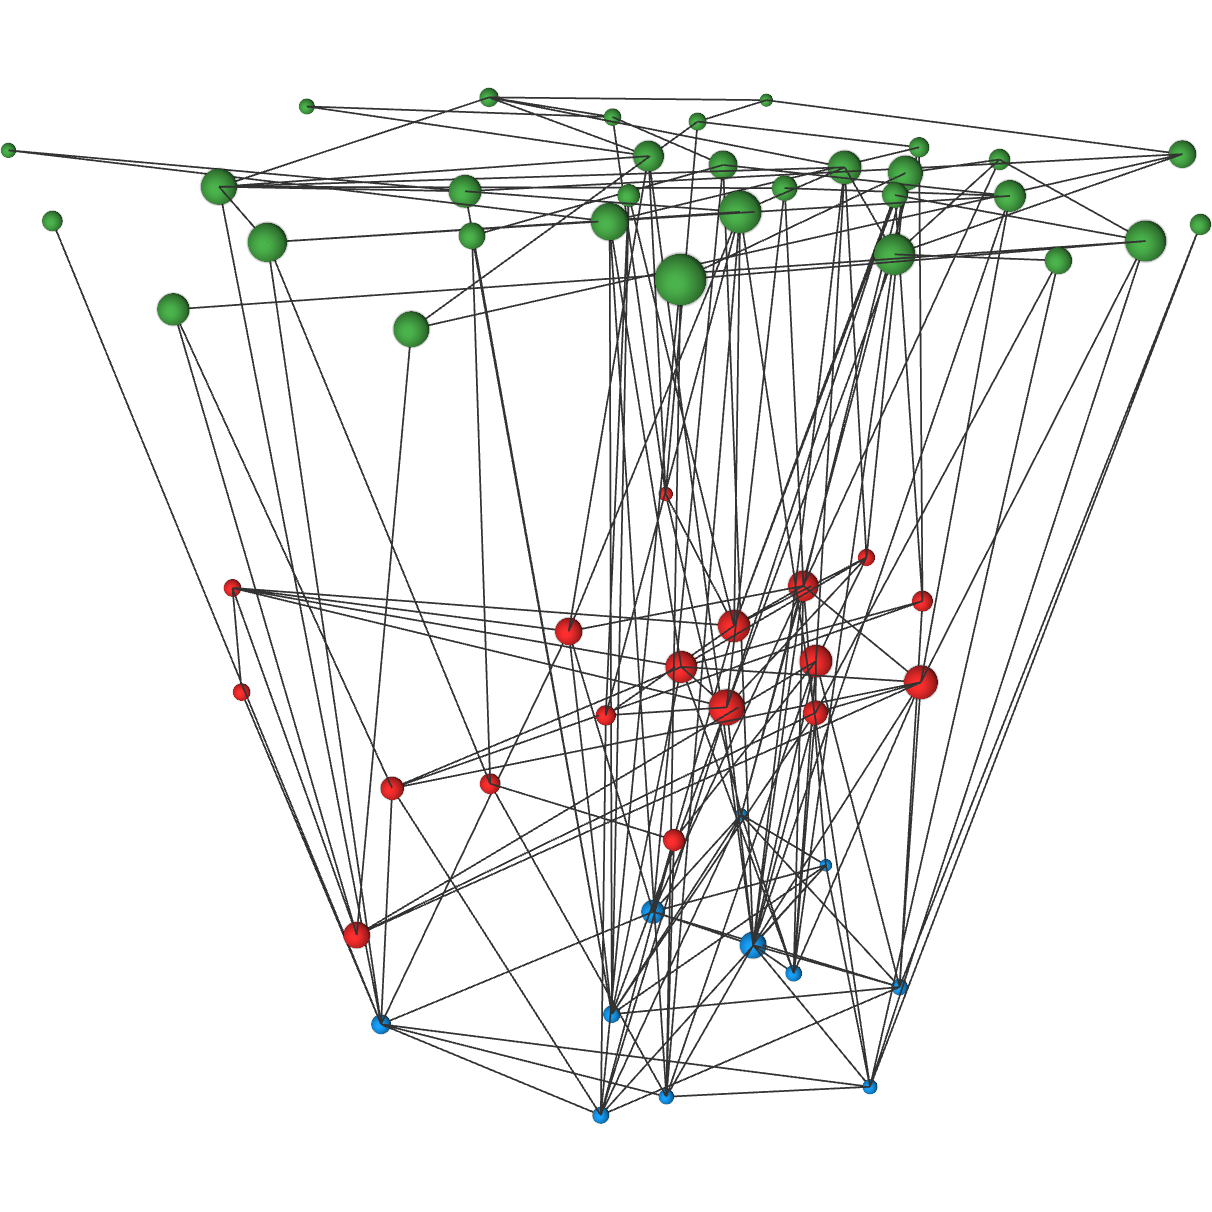
\includegraphics[width=\w,height=\h,keepaspectratio]{images/ex2/extruded}%
    }\\[5mm]
  \end{adjustwidth}  
  \caption[Different layouts for a graph with 3 domains, 60 nodes and 200 edges with a inter-/intra-domain edge ratio of 50\%.]{Different layouts obtained by applying different strategy and layout combinations to a graph with 3 domains, 60 nodes and 200 edges with an inter-/intra-domain edge ratio of 50\%.}%
  \label{fig:ex2}
\end{figure}
  \cleartoodd
}

\afterpage{%
    \cleartoodd
\begin{figure}[p]
  \begin{adjustwidth}{0cm}{-1cm}
    \setlength{\w}{0.48\linewidth}
    \setlength{\h}{0.35\textheight}
  \subfloat[Single strategy with \gls{2d} Fruchterman-Reingold layout]{%
		\label{fig:ex3-single}%
		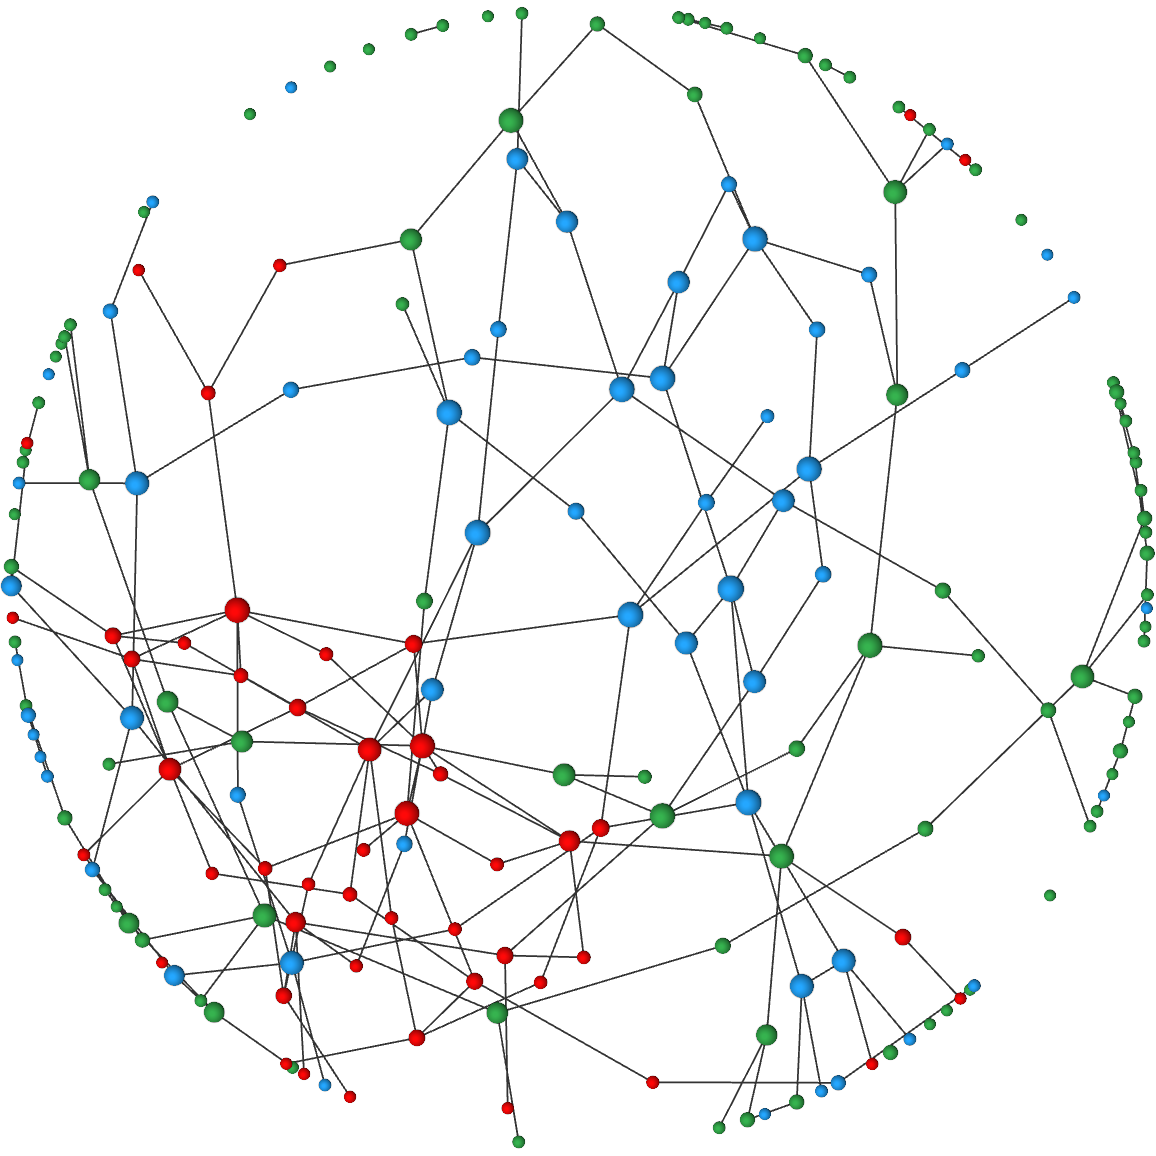
\includegraphics[width=\w,height=\h,keepaspectratio]{images/ex3/single}%
	}%
	\hfill
	\subfloat[Clustered strategy with \gls{2d} Fruchterman-Reingold layout]{%
		\label{fig:ex3-clustered}%
		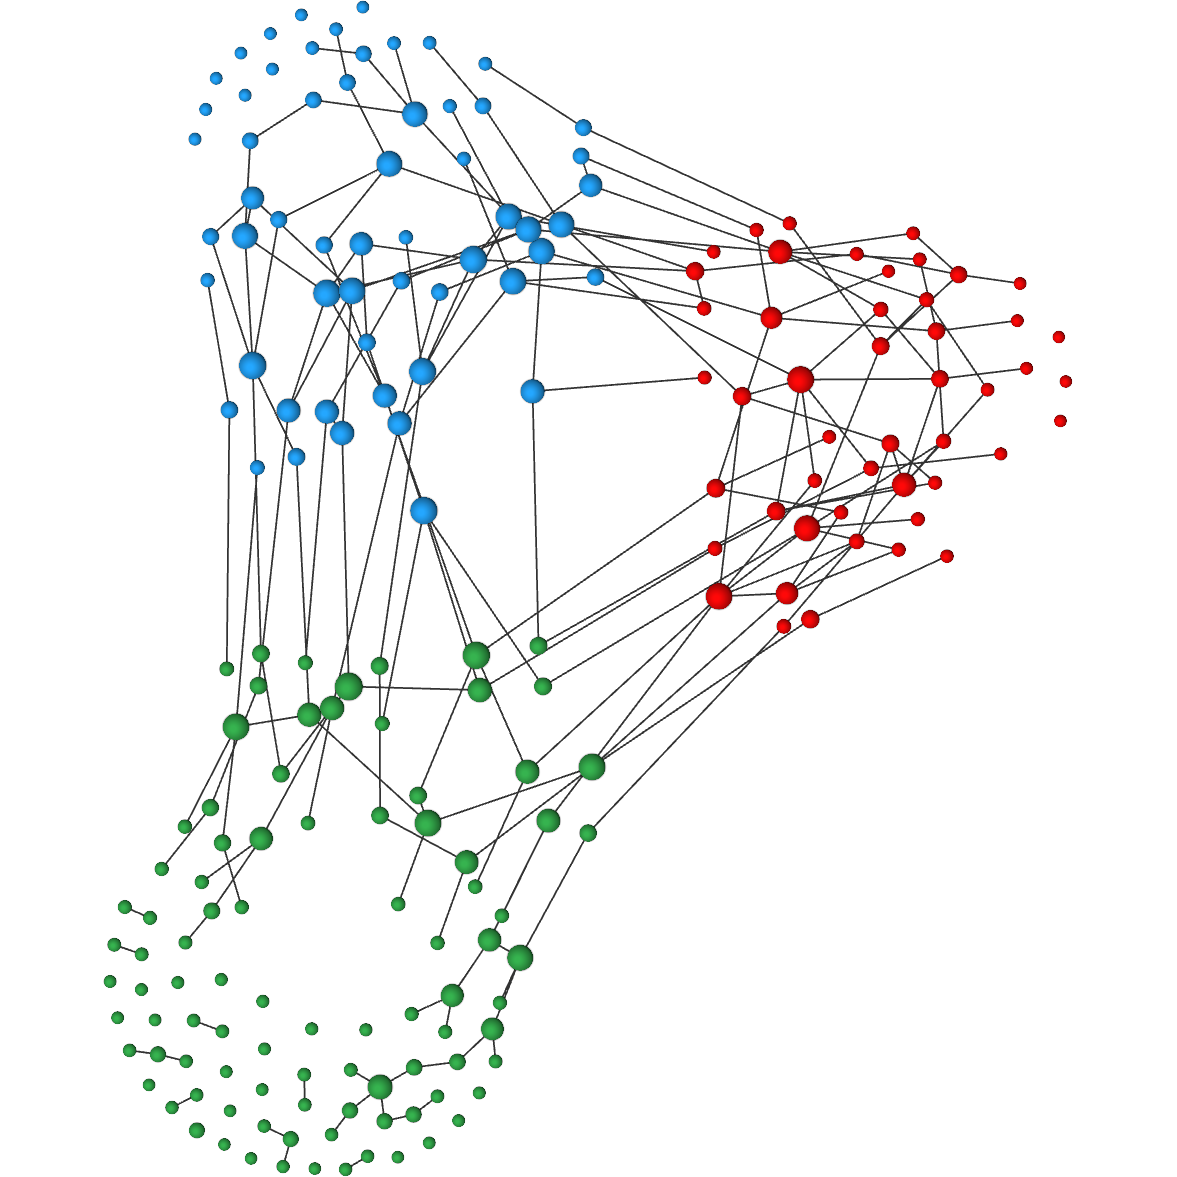
\includegraphics[width=\w,height=\h,keepaspectratio]{images/ex3/clustered}%
  }\\[5mm]
	\subfloat[Multilevel strategy with Stacked layout for the domain and \gls{2d} Fruchterman-Reingold layout for each layer]{%
		\label{fig:ex3-multilevel}%
		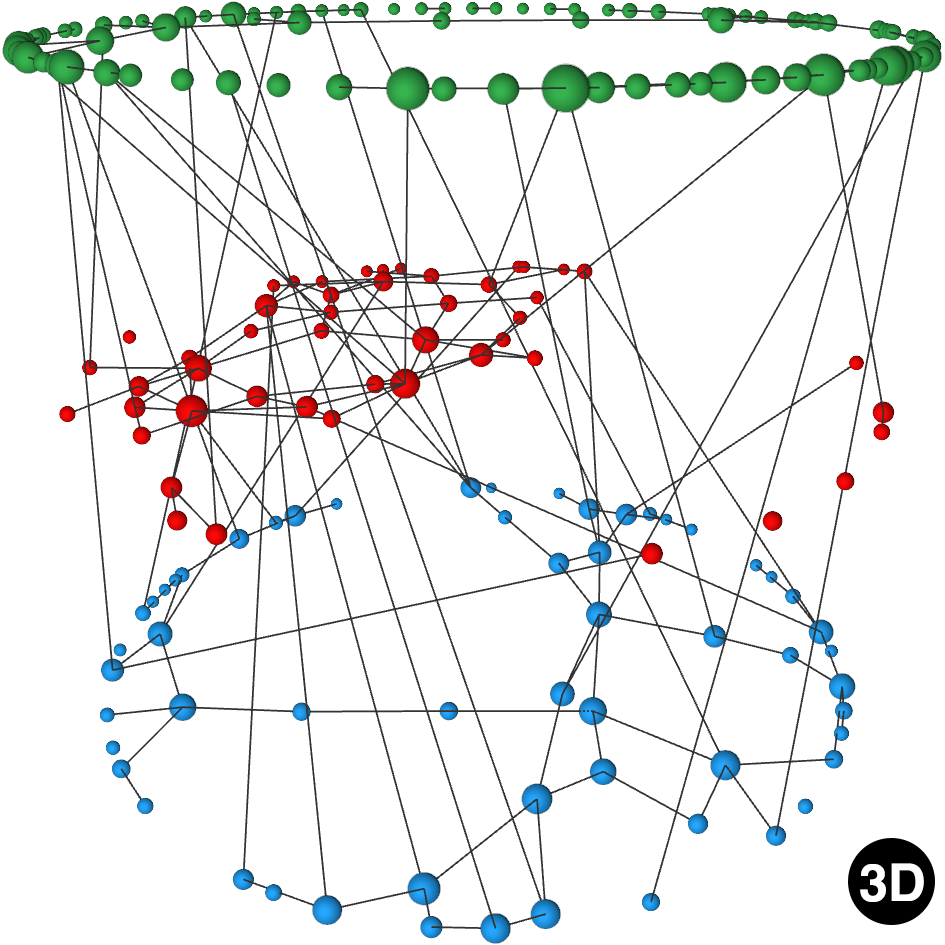
\includegraphics[width=\w,height=\h,keepaspectratio]{images/ex3/multilevel}%
  }
	\hfill
		\subfloat[Extruded strategy with Domain \gls{2d} Fruchterman-Reingold layout]{%
		\label{fig:ex3-extruded}%
		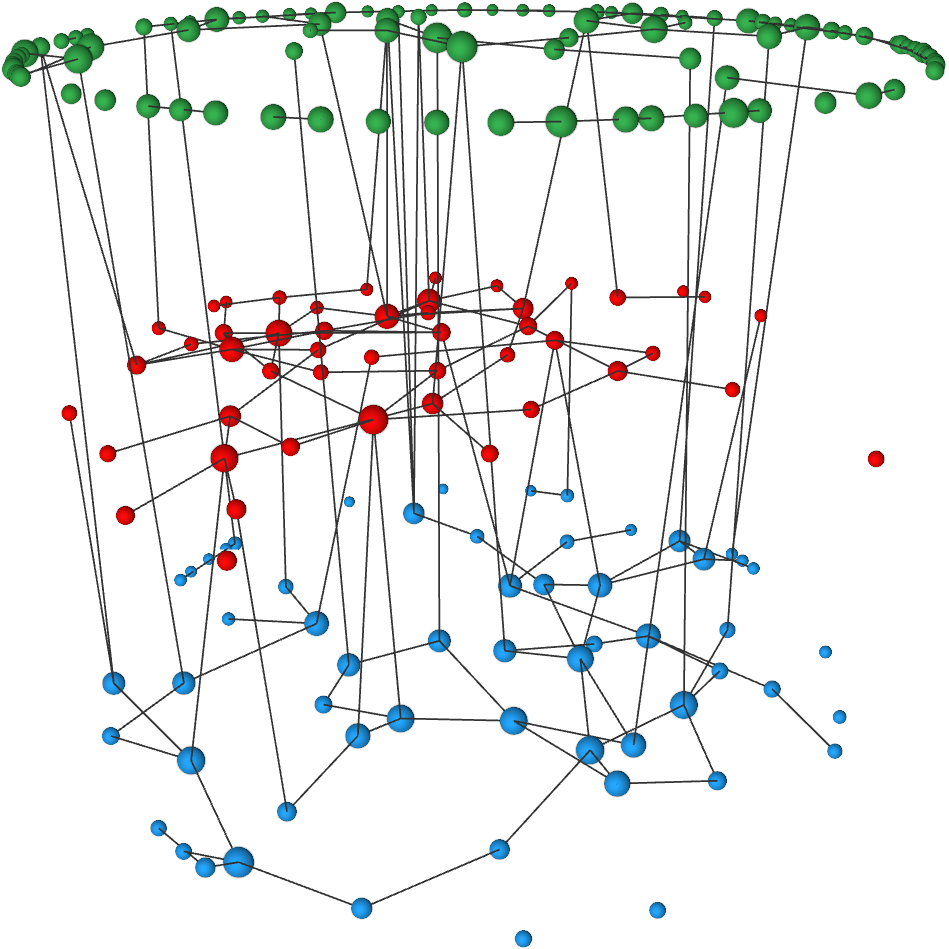
\includegraphics[width=\w,height=\h,keepaspectratio]{images/ex3/extruded}%
	}\\[5mm]
    \end{adjustwidth}  
  \caption[Different layouts for a graph with 3 domains, 200 nodes and 200 edges.]{Different layouts obtained by applying different strategy and layout combinations to a graph with 3 domains, 200 nodes and 200 edges.}%
  \label{fig:ex3}
\end{figure}
  \cleartoodd
}

\afterpage{%
  \cleartoodd
\begin{figure}[p]
  \begin{adjustwidth}{-0cm}{-1cm}  
        \setlength{\w}{0.48\linewidth}
    \setlength{\h}{0.35\textheight}
  \subfloat[Single strategy with \gls{2d} Fruchterman-Reingold layout]{%
		\label{fig:ex4-single}%
		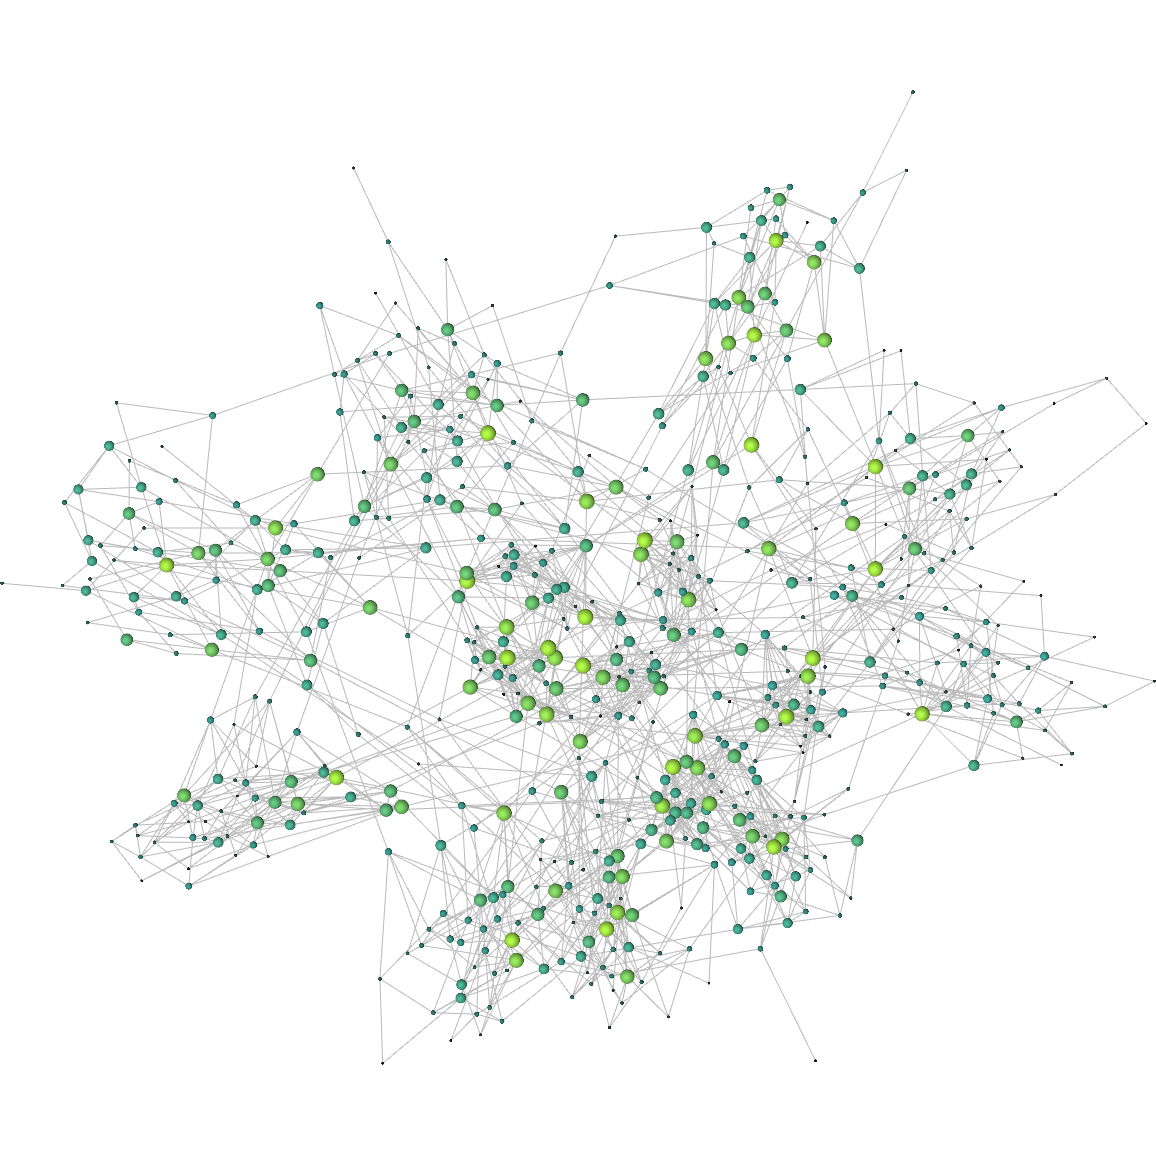
\includegraphics[width=\w,height=\h,keepaspectratio]{images/ex4/single}%
	}%
	\hfill
	\subfloat[Multilevel strategy with \gls{2d} Fruchterman-Reingold layout for both the inter- and intra-domain graphs]{%
		\label{fig:ex4-multilevel}%
		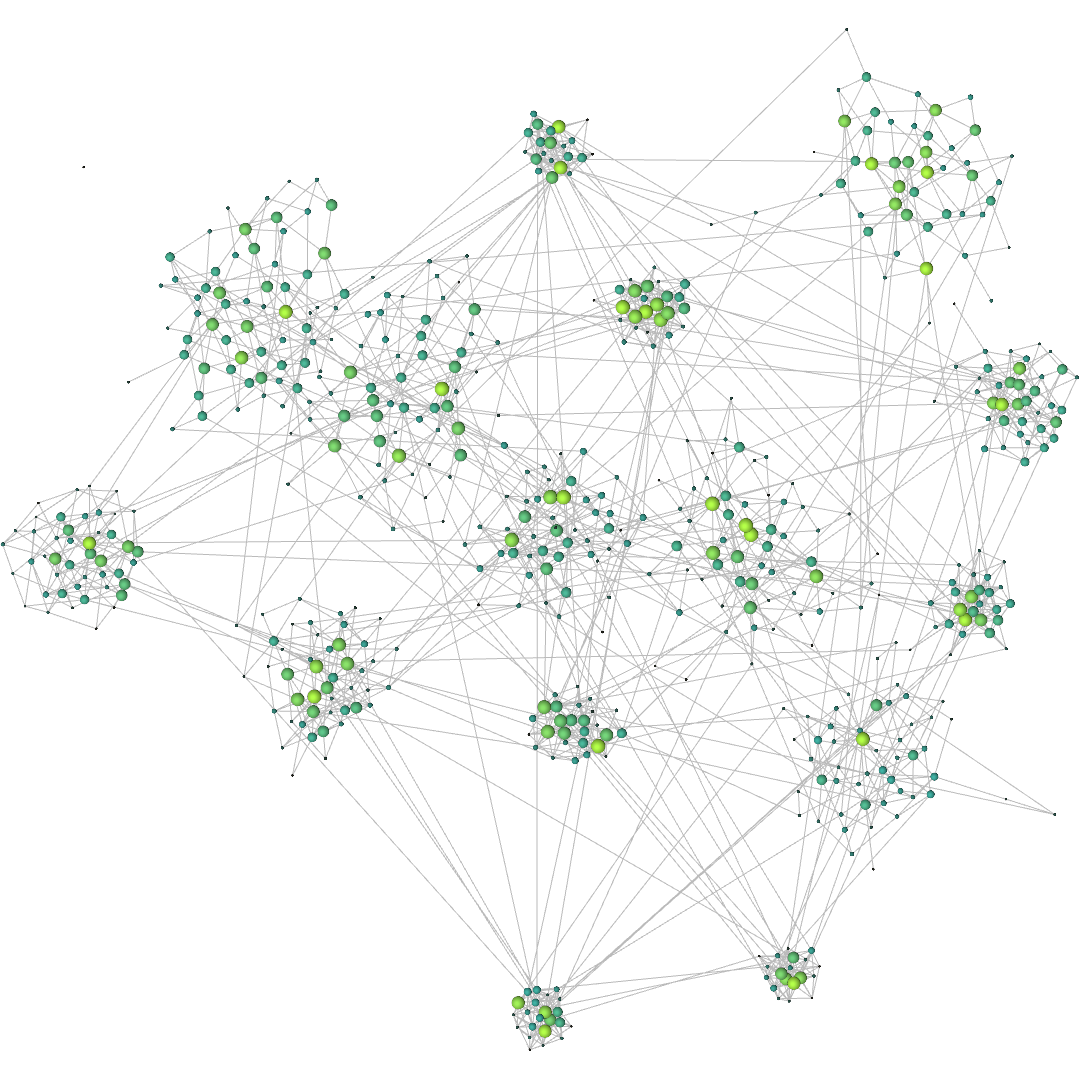
\includegraphics[width=\w,height=\h,keepaspectratio]{images/ex4/multilevel}%
  }\\[5mm]
	\subfloat[Extruded strategy with \gls{2d} Fruchterman-Reingold layout]{%
		\label{fig:ex4-extruded}%
		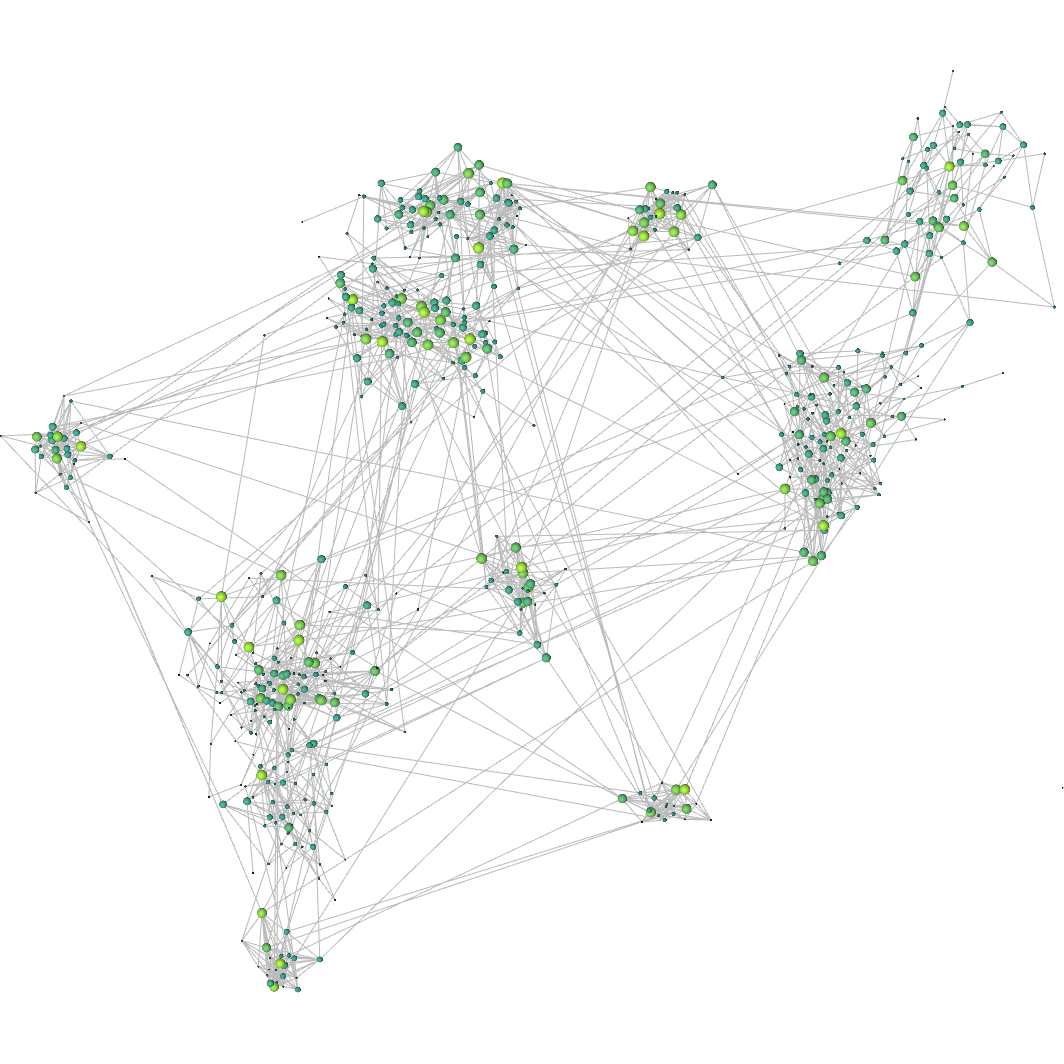
\includegraphics[width=\w,height=\h,keepaspectratio]{images/ex4/extruded}%
	}
	\hfill
  \subfloat[Clustered strategy with \gls{2d} Fruchterman-Reingold layout]{%
		\label{fig:ex4-clustered}%
		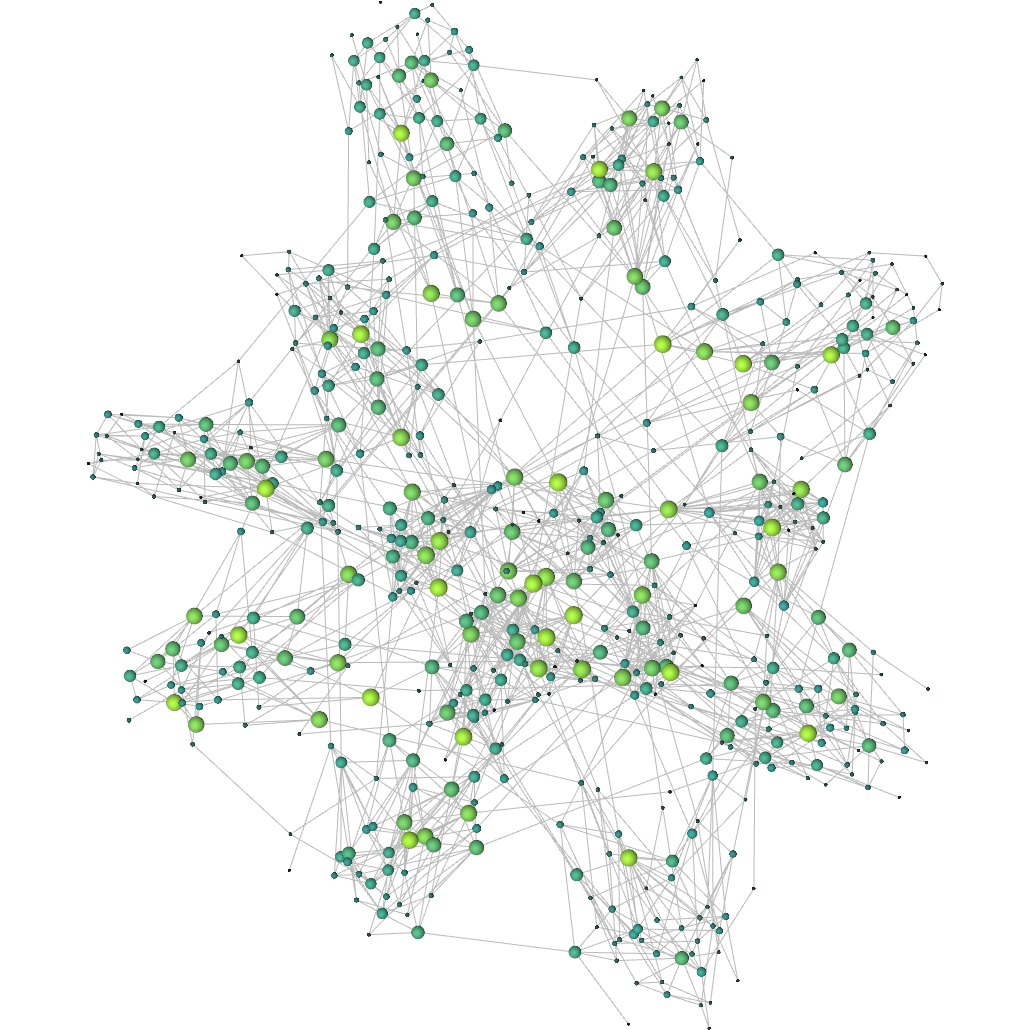
\includegraphics[width=\w,height=\h,keepaspectratio]{images/ex4/clustered}%
  }\\[5mm]
  \end{adjustwidth}  
  \caption[Different layouts for a graph with 15 domains, 600 nodes and 2000 edges with a inter-/intra-domain edge ratio of 93\%.]{Different layouts obtained by applying different strategy and layout combinations to a graph with 15 domains, 600 nodes and 2000 edges with an inter-/intra-domain edge ratio of 93\%.}%
  \label{fig:ex4}
\end{figure}
  \cleartoodd
}

\afterpage{%
    \cleartoodd
  \begin{landscape}
  \addtolength{\columnwidth}{2cm}
  \addtolength{\topmargin}{-2cm}
  \begin{figure}
    \captionsetup{
      format=hang,
      labelformat=simple,
      singlelinecheck=false,
      font={footnotesize,it},
      margin={0cm,2cm},
    }
    \subfloat[Intra-domain edge clarity preference]{%
      \label{fig:ex5-intra}%
      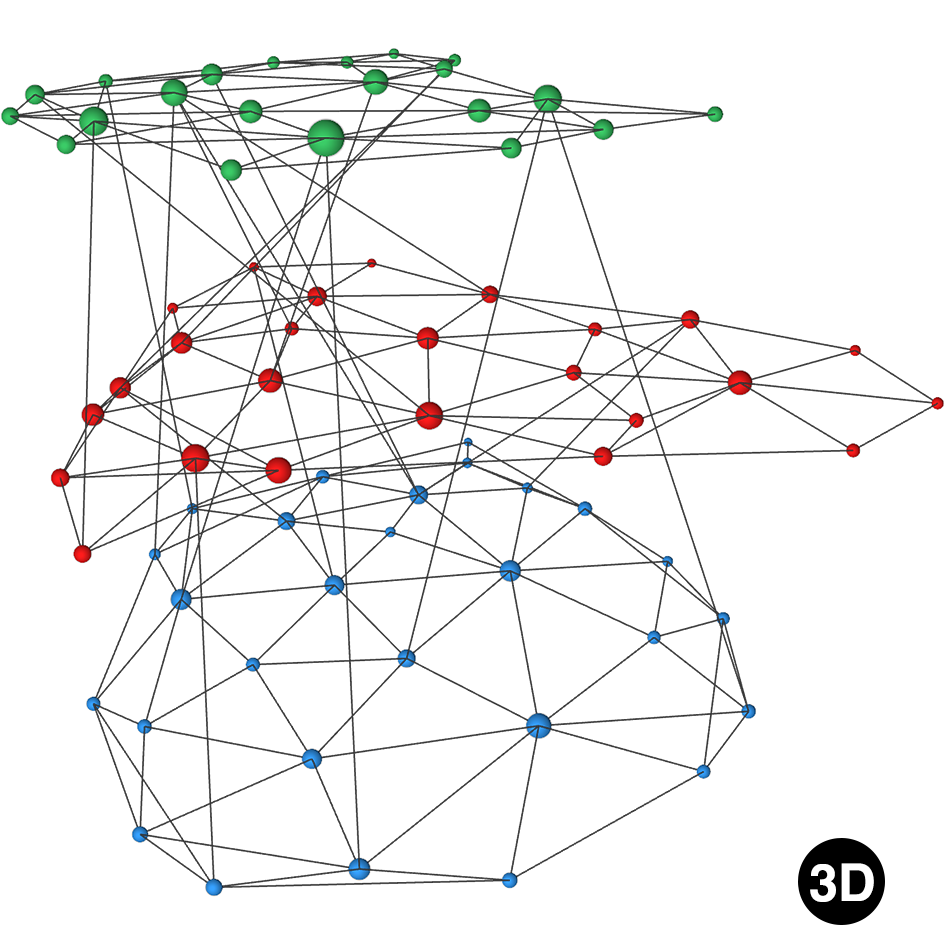
\includegraphics[width=0.32\linewidth]{images/ex5/multilevel-intra}%
    }\hfill
    \subfloat[Same preference for intra- or inter-domain clarity]{%
      \label{fig:ex5-middle}%
      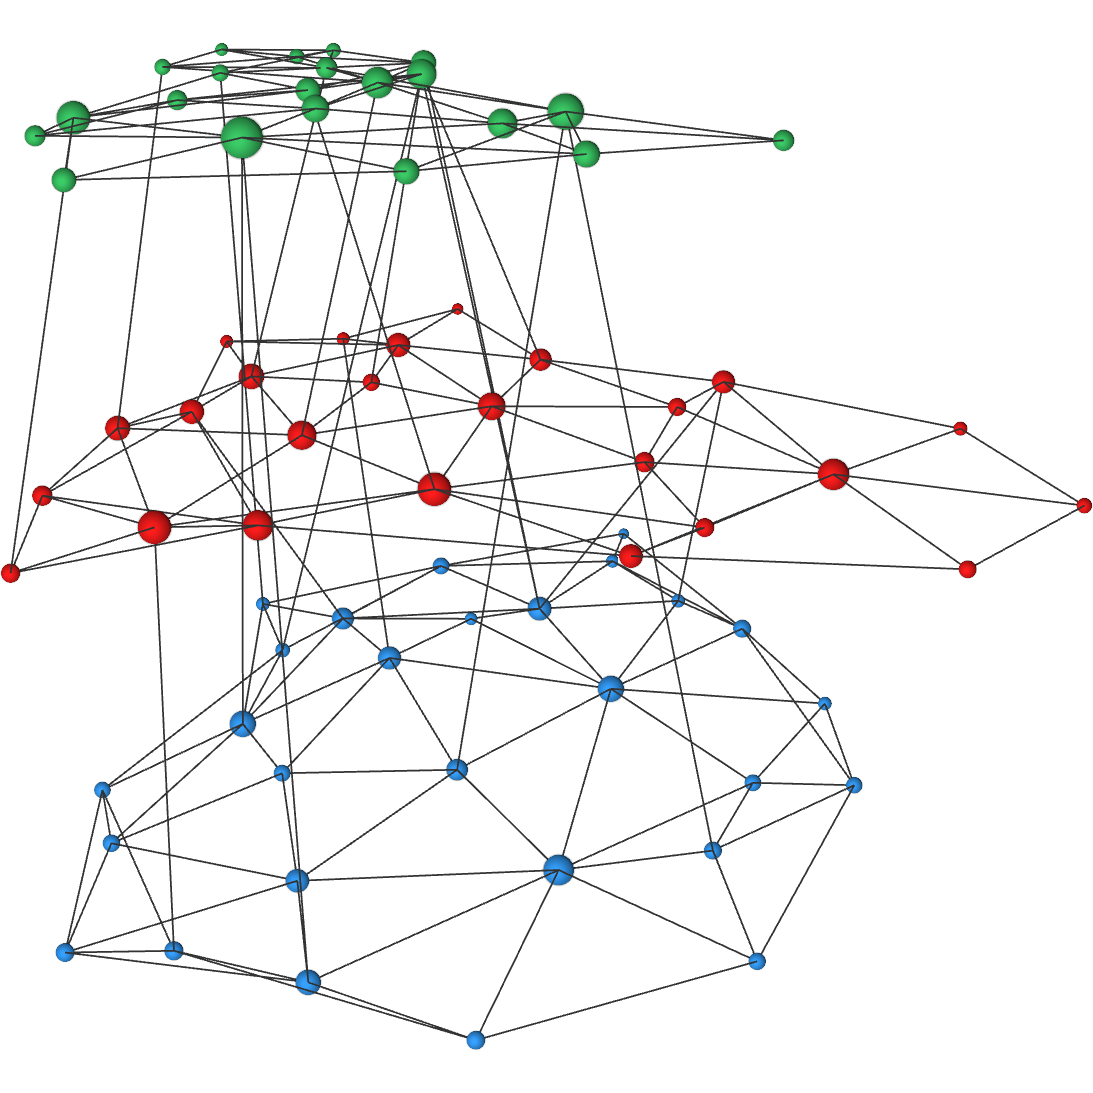
\includegraphics[width=0.32\linewidth]{images/ex5/multilevel-middle}%
    }\hfill
    \subfloat[Inter-domain edge clarity preference]{%
      \label{fig:ex5-inter}%
      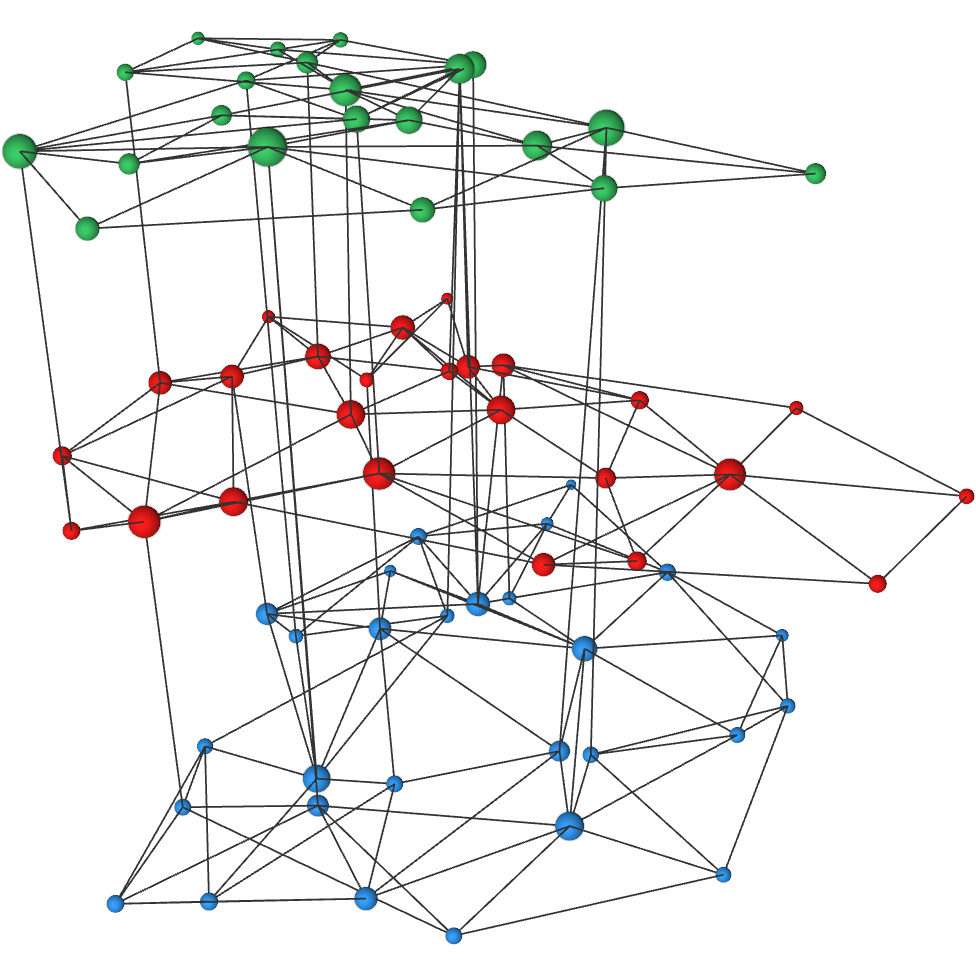
\includegraphics[width=0.32\linewidth]{images/ex5/multilevel-inter}%
    }\\[5mm]
    \caption[Effect of different values of the inter-/intra-domain layout clarity tradeoff.]{Different layouts obtained by changing the inter-/intra-domain layout clarity tradeoff of the Domain Fruchterman-Reingold \gls{2d} layout when applied to a graph with 3 domains, 74 nodes and 206 edges with an inter-/intra-domain edge ratio of 90\%. Each domain is a (planar) Delaunay triangulation.}%
    \label{fig:ex5}
    \clearpage
  \end{figure}
  \end{landscape}
    \cleartoodd
}
